\documentclass[12pt,a4paper]{report}

% --- Font & Language ---
\usepackage[T1]{fontenc}
\usepackage[utf8]{inputenc}
\usepackage{babel}
\babelprovide[main, import]{french}

% --- Margins ---
\usepackage[top=2.5cm, bottom=2.5cm, left=3cm, right=2.5cm]{geometry}

% --- Layout & Graphics ---
\usepackage{setspace}
\onehalfspacing
\usepackage{graphicx}
\usepackage{titlesec}
\usepackage{fancyhdr}
\usepackage{float}
\usepackage{longtable}
\usepackage{booktabs}
\usepackage{array}
\usepackage{listings}
\usepackage[table]{xcolor}
\usepackage{amsmath}
\usepackage{caption}
\usepackage{tocloft}
\usepackage{tabularx}
\usepackage{xltabular}

% --- TOC Customization ---
% Add dots for chapters
\renewcommand{\cftchapleader}{\cftdotfill{\cftdotsep}}

% --- Chapter Title Design ---
\titleformat{\chapter}[display]
  {\normalfont\Huge\bfseries\color{black}}
  {\filleft\textsf{\LARGE\chaptertitlename\ \thechapter}}
  {20pt}
  {\titlerule\vspace{1.5ex}\filcenter\Huge}
  [\vspace{1ex}\titlerule]

\titlespacing*{\chapter}{0pt}{50pt}{40pt}

% Prefix "Chapitre X : " in TOC
\renewcommand{\cftchappresnum}{Chapitre }
\renewcommand{\cftchapaftersnum}{ : }
\newlength{\chapnumwidth}
\settowidth{\chapnumwidth}{\bfseries Chapitre 99 : }
\addtolength{\cftchapnumwidth}{\chapnumwidth}

% Fix for ?contentsname? and ?listfigurename?
\addto\captionsfrench{%
  \renewcommand{\contentsname}{Table des matières}%
  \renewcommand{\listfigurename}{Liste des figures}%
  \renewcommand{\listtablename}{Liste des tableaux}%
}

% --- Hyperref (Should be loaded last) ---
\usepackage{hyperref}
\hypersetup{
    colorlinks=true,
    linkcolor=black,
    citecolor=blue,
    filecolor=magenta,      
    urlcolor=blue,
    pdftitle={Rapport de PFE - eduGenius},
    pdfauthor={Karim Joudi},
    pdfpagemode=UseOutlines,
}

% --- Code Syntax Highlighting ---
\definecolor{codegreen}{rgb}{0,0.6,0}
\definecolor{codegray}{rgb}{0.5,0.5,0.5}
\definecolor{codepurple}{rgb}{0.58,0,0.82}
\definecolor{backcolour}{rgb}{0.95,0.95,0.92}

\lstdefinelanguage{JavaScript}{
  keywords={break, case, catch, continue, debugger, default, delete, do, else, false, finally, for, function, if, in, instanceof, new, null, return, switch, this, throw, true, try, typeof, var, void, while, with, as, async, await, const, let, yield},
  morecomment=[l]{//},
  morecomment=[s]{/*}{*/},
  morestring=[b]',
  morestring=[b]",
  ndkeywords={class, export, boolean, throw, implements, import, this},
  keywordstyle=\color{blue}\bfseries,
  ndkeywordstyle=\color{darkgray}\bfseries,
  identifierstyle=\color{black},
  sensitive=false,
  commentstyle=\color{codegreen}\ttfamily,
  stringstyle=\color{codepurple}\ttfamily,
}

\lstdefinestyle{mystyle}{
    backgroundcolor=\color{backcolour},   
    commentstyle=\color{codegreen},
    keywordstyle=\color{magenta},
    numberstyle=\tiny\color{codegray},
    stringstyle=\color{codepurple},
    basicstyle=\ttfamily\footnotesize,
    breakatwhitespace=false,         
    breaklines=true,                 
    captionpos=b,                    
    keepspaces=true,                 
    numbers=left,                    
    numbersep=5pt,                  
    showspaces=false,                
    showstringspaces=false,
    showtabs=false,                  
    tabsize=2,
    language=JavaScript
}
\lstset{style=mystyle}
\setcounter{tocdepth}{2}
\setcounter{secnumdepth}{2}

\begin{document}
\selectlanguage{french}

% --- Preliminary Pages ---
\pagenumbering{roman}
\newcommand{\HRule}{\rule{\linewidth}{0.5mm}}

\begin{titlepage}
    \begin{center}
        
\includegraphics[width=4cm]{images/logo-polytech.png} \\[1cm]
        
        \textsc{\Large Polytech-Intl : École Polytechnique Internationale}\\[0.5cm]
        \textsc{\large Département Informatique}\\[1.5cm]

        % Title
        \HRule \\[0.4cm]
        { \huge \bfseries \setstretch{1.3} eduGenius : Plateforme Éducative Intelligente Intégrant l'IA et la Visioconférence en Temps Réel \par}
        \vspace{0.2cm}
        \HRule \\[1.5cm]

        % Company
        \textsc{\Large Organisme d'Accueil : BES2I}\\[0.2cm]
        \textsc{\large Business Expert Software \& Systems Integrator}\\[1cm]

        % Authors
        \begin{minipage}{0.4\textwidth}
            \begin{flushleft} \large
                \emph{Réalisé par :}\\
                Karim \textsc{Joudi}
            \end{flushleft}
        \end{minipage}
        ~
        \begin{minipage}{0.4\textwidth}
            \begin{flushright} \large
                \emph{Encadré par :} \\
                Mme. Imen Msakni
            \end{flushright}
        \end{minipage}\\[3cm]

        % Degree
        \large \textit{Rapport de Projet de Fin d'Études présenté en vue de l'obtention du}\\[0.2cm]
        \textbf{Diplôme National d'Ingénieur en Génie Logiciel}\\[2cm]

        \vfill

        % Bottom of the page
        {\large Année Universitaire : 2025 - 2026}
    \end{center}
\end{titlepage}

\clearpage
\chapter*{Dédicaces}
\phantomsection
\addcontentsline{toc}{chapter}{Dédicaces}
\begin{center}
    \textit{À ma chère famille,} \\
    \textit{Votre amour inconditionnel et votre soutien ont été mon moteur.} \\
    \vspace{1cm}
    \textit{À mes professeurs,} \\
    \textit{Merci pour votre guidance et votre savoir.} \\
    \vspace{1cm}
    \textit{À tous les passionnés d'éducation et de technologie,} \\
    \textit{Ce travail est pour vous.}
\end{center}

\clearpage
\chapter*{Remerciements}
\phantomsection
\addcontentsline{toc}{chapter}{Remerciements}

Je tiens à exprimer ma profonde gratitude à l'ensemble des personnes qui ont contribué au succès de ce projet et à mon épanouissement durant ce stage.

Tout d'abord, je remercie mon encadrant professionnel au sein de \textbf{BES2I} pour sa confiance, son expertise technique et ses précieux conseils qui m'ont permis de mener à bien le développement d'eduGenius.

Mes remerciements s'adressent également à l'administration de l'École Polytechnique Internationale (\textbf{Polytech-Intl}) pour m'avoir offert l'opportunité de travailler sur un projet aussi innovant et pour la qualité de la formation que j'ai reçue.

Je tiens à remercier les membres du jury pour l'honneur qu'ils me font en acceptant d'évaluer ce travail.

Enfin, je remercie ma famille et mes amis pour leur soutien constant et leurs encouragements tout au long de mon parcours académique.

\clearpage

% --- Table of Contents ---
\phantomsection
\addcontentsline{toc}{chapter}{Table des matières}
\tableofcontents
\clearpage

% --- Lists ---
\phantomsection
\addcontentsline{toc}{chapter}{Liste des figures}
\listoffigures
\clearpage

\phantomsection
\addcontentsline{toc}{chapter}{Liste des tableaux}
\listoftables
\clearpage

\pagenumbering{arabic}

% --- Chapters ---
\chapter*{Introduction Générale}
\phantomsection
\addcontentsline{toc}{chapter}{Introduction Générale}

À l'ère de la quatrième révolution industrielle, le secteur de l'éducation connaît une mutation profonde portée par la convergence de l'intelligence artificielle et des technologies de collaboration en temps réel \cite{ai_education}. Cette transformation numérique ne se limite plus à la simple numérisation des supports pédagogiques, mais vise désormais à résoudre le défi majeur de l'enseignement moderne : passer d'un apprentissage passif et uniforme à une expérience active, immersive et personnalisée.

C'est dans ce contexte de rupture technologique que s'inscrit notre Projet de Fin d'Études intitulé \textbf{EduGenius}. Ce projet consiste en la conception et la réalisation d'une plateforme d'apprentissage de nouvelle génération qui fusionne les capacités de l'Intelligence Artificielle (IA) avec des outils de communication synchrone. L'ambition de cette solution est de redéfinir la relation entre l'apprenant, l'enseignant et le savoir en automatisant les tâches à faible valeur ajoutée pour se concentrer sur l'accompagnement pédagogique et la réussite académique.

La plateforme \textbf{EduGenius} est conçue comme un écosystème intégré répondant aux besoins de trois acteurs clés : l'administration, les enseignants et les étudiants. Elle se distingue par l'intégration native de moteurs d'IA pour la génération automatique de supports (résumés, quiz et flashcards), un module de visioconférence haute fidélité avec détection automatique de présence, et un système d'analyses avancées permettant de suivre proactivement les performances des apprenants. En s'appuyant sur des dynamiques de gamification, le projet vise non seulement à faciliter la transmission des connaissances, mais aussi à maximiser l'engagement et la rétention sur le long terme.

Le développement de cette solution a été mené selon une \textbf{démarche Agile (Scrum)}, garantissant une flexibilité maximale face aux défis techniques liés au traitement de données en temps réel et à l'intégration des modèles de langage. Cette méthodologie nous a permis de livrer des incréments fonctionnels réguliers tout en assurant une rigueur logicielle conforme aux standards de l'ingénierie moderne.

Le présent rapport documente l'ensemble du cycle de vie du projet, structuré autour des axes suivants :

\begin{itemize}
    \item \textbf{Chapitre 1 : Cadre général du projet} -- expose la problématique, les objectifs stratégiques, l'étude comparative des solutions du marché ainsi que le cadre méthodologique retenu.
    \item \textbf{Chapitre 2 : Analyse et Spécification des besoins} -- définit les exigences fonctionnelles et non-fonctionnelles à travers une modélisation rigoureuse des besoins utilisateurs.
    \item \textbf{Chapitre 3 : Conception de la solution} -- détaille l'architecture logicielle, la conception de la base de données et les choix de design système.
    \item \textbf{Chapitre 4 : Réalisation et Mise en œuvre} -- présente l'environnement technique, les technologies utilisées (Stack MERN) et les fonctionnalités clés implémentées.
    \item \textbf{Chapitre 5 : Tests et Évaluation} -- récapitule les phases de validation, les tests de performance et les résultats obtenus par rapport aux objectifs initiaux.
\end{itemize}
\chapter{Contexte et Cadrage Stratégique}

\section*{Introduction}
Ce chapitre inaugural constitue le socle stratégique de notre étude. L'objectif est de situer le projet EduGenius non seulement dans son environnement technique, mais aussi dans sa réalité organisationnelle. Nous débuterons par une immersion au sein de l'organisme d'accueil afin d'appréhender son "ADN numérique" et les expertises métier qui ont jalonné le développement de cette solution. Cette compréhension est indispensable pour justifier les choix architecturaux et technologiques qui seront détaillés dans les phases ultérieures de ce rapport.

\section{Immersion au sein de l’organisme d’accueil}
L'innovation logicielle est le reflet de la culture qui la porte. Le projet EduGenius a été conçu au sein de BES2I, un cabinet de conseil et d'expertise technologique dont la philosophie repose sur l'alliance entre l'excellence technique et l'aventure humaine.

\subsection{Vision et Stratégie de l'entreprise : L'Esprit BES2I}
BES2I se définit comme un "accélérateur de transformation digitale" dont la mission dépasse la simple prestation technique. Sa vision repose sur trois piliers fondamentaux : la proximité avec ses partenaires, l'agilité opérationnelle et l'engagement envers la réussite des projets.

Contrairement aux grandes structures impersonnelles, BES2I cultive un ADN marqué par une forte réactivité et une capacité à intervenir sur des problématiques à haute valeur ajoutée. L'entreprise prône une transformation digitale durable et raisonnée, où chaque ligne de code doit servir un objectif métier précis. C'est cet esprit entrepreneurial et cette culture de "Software Craftsmanship" qui ont permis de donner naissance à un projet ambitieux comme EduGenius, conçu pour humaniser l'apprentissage numérique.

\subsection{Écosystème de compétences}
L’organisation de BES2I est structurée pour offrir un accompagnement de bout en bout, de la réflexion stratégique au déploiement opérationnel.

\subsubsection{Pôle Ingénierie \& Développement Cloud}
Ce pôle représente le cœur d'expertise technique de l'entreprise. Spécialisé dans le développement sur-mesure et les architectures modernes (Cloud, Web, Mobile), il garantit la conception de solutions robustes et évolutives. Pour EduGenius, ce pôle a apporté la maîtrise des frameworks de dernière génération (Stack MERN) et des protocoles de communication temps réel, assurant une plateforme fluide capable de supporter des charges d'utilisateurs simultanés.

\subsubsection{Division IA \& Intelligence Cognitive}
Au cœur de la stratégie d'innovation de BES2I, cette division explore les applications concrètes de l'intelligence artificielle générative. Elle transforme les concepts théoriques en fonctionnalités tangibles : automatisation de la rédaction, analyse prédictive des données et personnalisation de l'expérience utilisateur. Cette expertise a été le moteur du module IA d'EduGenius, permettant la génération automatisée de ressources pédagogiques (résumés, quiz) et l'adaptation du parcours au rythme de l'étudiant.

\subsection{Rayonnement et enjeux concurrentiels}
Dans un marché de l’EdTech (Education Technology) en pleine mutation, BES2I se positionne comme un créateur de solutions disruptives. Son rayonnement repose sur sa capacité à proposer des outils qui ne sont pas de simples référentiels de documents, mais de véritables écosystèmes interactifs.

L’enjeu concurrentiel pour BES2I est de démontrer qu'une expertise pointue en ingénierie peut radicalement améliorer l'engagement étudiant. En intégrant l'IA et le collaboratif synchrone au sein d'une même plateforme, l'entreprise se démarque des solutions "legacy" souvent trop rigidies, affirmant ainsi sa position de leader dans la conception de logiciels à fort impact social et éducatif.

\section{Genèse et Enjeux du Projet}

La conception d'EduGenius ne relève pas d'une simple volonté de numérisation, mais d'une réponse stratégique aux mutations structurelles de l'éducation globale et aux nouvelles exigences de performance académique. Ce projet vise à redéfinir la relation entre l'apprenant, le formateur et l'outil numérique en plaçant l'engagement et l'intelligence au cœur du système.

\subsection{Contexte du Projet EduGenius}
Le projet EduGenius s'inscrit dans un paysage éducatif marqué par l'accélération numérique post-crise sanitaire. Si la période de pandémie a imposé l'usage d'outils de fortune pour assurer la continuité, l'ère actuelle exige une \textbf{professionnalisation des environnements numériques d'apprentissage (ENA)}.

Aujourd'hui, l'enseignement hybride est devenu une modalité pédagogique de choix. Cependant, la dispersion actuelle des outils — un logiciel pour la vidéo, un autre pour les documents, un troisième pour les quiz — crée une "fatigue numérique" et une fragmentation critique des données. EduGenius naît de la volonté de \textbf{BES2I} d'unifier ces silos technologiques dans un écosystème cohérent, capable de supporter une charge importante d'utilisateurs tout en offrant une expérience fluide, souveraine et sécurisée, conforme aux standards du Web moderne.

\subsection{Diagnostic de la Problématique}
L'analyse menée lors de la phase de cadrage a permis d'identifier des points de rupture critiques au sein des plateformes conventionnelles. Le diagnostic révèle que les échecs du e-learning actuel sont autant ergonomiques que pédagogiques.

\begin{itemize}
    \item \textbf{L’austérité visuelle et l’obsolescence de l’UX :} La majorité des plateformes actuelles (LMS classiques) souffrent d'une interface austère et d'une ergonomie rigide. Cette absence de soin apporté à l'interface utilisateur (UI) crée une barrière psychologique dès la connexion. Pour la génération "Digital Native", une plateforme visuellement peu attrayante est perçue comme un outil de contrainte plutôt qu'un espace de découverte.
    
    \item \textbf{L’apprentissage passif et l'absence de stimuli ludiques :} Le modèle traditionnel de consommation de contenu favorise la passivité. L'absence d'un \textbf{"Game Hub"} ou de mécanismes de gamification rend le parcours linéaire et monotone. Sans défis progressifs ou sentiment de récompense, l'étudiant perd rapidement sa motivation, justifiant l'introduction de zones d'interactivité ludique pour maintenir un éveil cognitif élevé.

    \item \textbf{Le fardeau administratif et le manque d'assistance intelligente :} Les enseignants consacrent une part disproportionnée de leur temps à des tâches répétitives : résumé de chapitres et conception de questionnaires. Parallèlement, l'étudiant se retrouve souvent seul face à des documents denses. L'absence de briques d'intelligence artificielle intégrées crée une latence pédagogique qui nuit à la fluidité de l'apprentissage.
\end{itemize}

\subsection{Vision Cible et Objectifs SMART}
La vision d'EduGenius est de devenir le hub central de l'apprentissage "Intelligent-First" et "User-Centric". Cette ambition se traduit par des objectifs rigoureux :

\begin{itemize}
    \item \textbf{Spécifique :} Concevoir une plateforme web intégrée (All-in-One) alliant modernité visuelle et puissance technologique via trois piliers :
    \begin{enumerate}
        \item \textit{Intelligence Artificielle Souveraine :} Intégration d'\textbf{Ollama} pour fournir une assistance à la génération de résumés et de quiz, garantissant la confidentialité absolue des données.
        \item \textit{Collaboration Synchrone Immersive :} Exploitation du \textbf{SDK Daily.co} pour offrir une expérience de visioconférence fluide et stable.
        \item \textit{Ludo-pédagogie (Game Hub) :} Implémentation d'un espace dédié à la gamification pour transformer l'apprentissage en un parcours de réussite stimulant.
    \end{enumerate}

    \item \textbf{Mesurable :} 
    \begin{itemize}
        \item Optimiser la productivité des formateurs en divisant par trois le temps consacré à la synthèse de documents grâce à l'assistance générative locale.
        \item Garantir une qualité de flux vidéo HD constante avec une latence minimale via l'infrastructure managée de Daily.co.
        \item Augmenter le temps de rétention des étudiants sur la plateforme de \textbf{40 \%} grâce à l'attractivité du Game Hub.
    \end{itemize}

    \item \textbf{Atteignable :} La faisabilité repose sur l'utilisation d'une stack technologique de pointe (Next.js, Tailwind CSS et Ollama), assurant un développement agile et performant.

    \item \textbf{Pertinent :} Le projet répond aux nouveaux standards de l'EdTech en offrant une solution souveraine qui traite le problème de l'engagement étudiant par le design et l'IA.

    \item \textbf{Temporel :} Le projet suit un cycle de développement structuré en sprints, avec une livraison finale prévue au terme de la période de stage.
\end{itemize}

\section{État de l’Art et Analyse Critique}

L'évolution des technologies éducatives (EdTech) a transformé les méthodes de transmission du savoir. Cependant, l'analyse du paysage actuel révèle une fracture importante entre les capacités techniques disponibles et l'expérience utilisateur réelle. Cette section dresse un panorama critique des solutions existantes pour justifier le positionnement disruptif d'EduGenius.

\subsection{Étude de l’existant}
L'écosystème numérique d'apprentissage actuel est marqué par une forte fragmentation. Les établissements utilisent généralement une combinaison de trois types d'outils : des systèmes de gestion (LMS), des outils de communication synchrone (Visioconférence) et des outils de gestion administrative comme \textbf{KEDUX}.

Bien que performantes dans leurs domaines respectifs, ces solutions fonctionnent en "silos". L'apprenant doit constamment basculer d'un environnement à un autre (Context Switching), ce qui entraîne une déperdition d'information, une baisse de la concentration et une charge cognitive inutile. Le manque d'intégration native de l'intelligence artificielle et l'austérité des interfaces restent les obstacles majeurs à une adoption fluide.

\subsection{Benchmark des solutions du marché}
Afin de positionner EduGenius, nous avons réalisé une étude comparative basée sur les leaders du marché, segmentés en deux catégories : les LMS traditionnels et les outils axés sur l'engagement. Le tableau suivant synthétise les points de différenciation majeurs :

\begin{table}[H]
\centering
\resizebox{\textwidth}{!}{
\begin{tabular}{|l|c|c|c|c|}
\hline
\textbf{Fonctionnalités} & \textbf{LMS Classiques} & \textbf{Outils "Gamified"} & \textbf{Teams/Meet} & \textbf{EduGenius} \\ 
 & (Moodle, Canvas) & (Kahoot, Duolingo) & (Collaboratif) & (Notre Solution) \\ \hline
\textbf{IA Générative Native} & Non / Plugins tiers & Partielle & Non & \textbf{Oui (Gemini)} \\ \hline
\textbf{Gamification Profonde} & Faible & \textbf{Excellente} & Nulle & \textbf{Avancée} \\ \hline
\textbf{Visioconférence Native} & Non (Intégration) & Non & \textbf{Oui} & \textbf{Oui (Daily.co)} \\ \hline
\textbf{Quiz \& Résumés Auto} & Manuel uniquement & Manuel & Non & \textbf{Automatisé} \\ \hline
\textbf{Chat Temps Réel} & Basique & Non & \textbf{Avancé} & \textbf{Intégré} \\ \hline
\textbf{Suivi d'Assiduité} & Manuel / Logs & Non & Partiel & \textbf{Automatique} \\ \hline
\end{tabular}
}
\caption{Analyse comparative d'EduGenius face aux solutions existantes}
\end{table}

\subsubsection{Analyse des LMS Traditionnels (Moodle, Canvas, KEDUX)}
Les Learning Management Systems (LMS) sont les piliers de l'éducation numérique depuis deux décennies.
\begin{itemize}
\item \textbf{Points Forts :} Une gestion rigoureuse des cursus, des inscriptions et des notes. KEDUX, par exemple, excelle dans la gestion administrative des institutions académiques tunisiennes.
\item \textbf{Limites Critiques :} Ces plateformes sont souvent perçues comme des "dépôts de fichiers". L'ergonomie est centrée sur l'administration et non sur l'apprenant. L'interface est rigide, souvent datée, et ne propose aucun mécanisme d'engagement profond, ce qui favorise un apprentissage passif et un taux de décrochage élevé.
\end{itemize}

\subsubsection{Analyse des outils "Engage-Tech" (Kahoot, Duolingo)}
À l'opposé des LMS, ces outils se concentrent exclusivement sur la rétention et le plaisir de l'utilisateur.
\begin{itemize}
\item \textbf{Points Forts :} Utilisation massive de la dopamine via des badges, des classements et des interfaces colorées. Le taux d'engagement est extrêmement élevé.
\item \textbf{Limites Critiques :} Ils manquent de "profondeur académique". Ce sont des outils périphériques qui ne permettent pas d'héberger un cours complet, de gérer des interactions vidéo professionnelles ou de traiter des données pédagogiques complexes. Ils ne peuvent pas constituer l'environnement de travail principal d'un étudiant.
\end{itemize}

\subsection{Identification du Gap Technologique}
L'analyse comparative met en évidence un "fossé technologique" sur trois axes majeurs :

\begin{enumerate}
\item \textbf{Le Verrou de la Souveraineté IA :} Les solutions actuelles qui intègrent l'IA dépendent quasi-exclusivement d'API Cloud (OpenAI, Anthropic). Cela pose des problèmes de coûts prohibitifs à l'échelle d'une institution et, surtout, des risques de fuite de données pédagogiques sensibles. L'absence d'IA locale (\textit{On-Premise}) est un manque critique.
\item \textbf{L'Instabilité des flux synchrones :} Les solutions WebRTC "maison" sont souvent peu fiables. La plupart des LMS délèguent cette partie à des outils tiers (Zoom, Meet), brisant ainsi l'unité de la plateforme.
\item \textbf{L'Érosion de la Motivation :} Aucune solution leader ne parvient à marier le sérieux d'un cursus académique (LMS) avec l'attractivité d'un environnement ludique (Game Hub), créant une "fatigue digitale" chez les étudiants.
\end{enumerate}

\subsection{Synthèse et Proposition de Valeur}
EduGenius se positionne comme un ENA (Environnement Numérique d'Apprentissage) de troisième génération. Notre proposition de valeur repose sur la convergence inédite de quatre piliers :

\begin{itemize}
\item \textbf{Intelligence Cognitive Souveraine :} Grâce à l'intégration d'\textbf{Ollama}, nous offrons une assistance IA puissante (résumés, quiz) dont les données ne quittent jamais le serveur local.
\item \textbf{Fluidité Native :} L'utilisation du \textbf{SDK Daily.co} permet d'intégrer une visioconférence de classe industrielle directement dans le parcours de cours, sans redirection externe.
\item \textbf{Engagement par le Design :} Une interface moderne sous \textbf{Next.js} couplée à un \textbf{Game Hub} pour transformer l'effort académique en un défi stimulant.
\item \textbf{Complémentarité Stratégique :} Là où KEDUX gère l'aspect administratif, EduGenius gère l'expérience d'apprentissage. Nous passons d'un outil de \textit{gestion} à un outil d'\textit{immersion}.
\end{itemize}

\section{Ingénierie du Périmètre et Acteurs}

La réussite d'un projet d'envergure tel qu'EduGenius repose sur une définition stricte de son périmètre d'action et une identification claire des interactions entre ses différents acteurs. Cette section détaille l'organisation fonctionnelle du système et la structure de gouvernance associée.

\subsection{Cartographie Fonctionnelle (The 6 Pillars)}

Le périmètre d'EduGenius s'articule autour de six piliers fondamentaux qui garantissent une expérience d'apprentissage complète, centralisée et technologiquement avancée :

\begin{enumerate}
\item \textbf{Identity and Access Management (IAM) :} Ce pilier assure la gestion sécurisée des authentifications et la segmentation des rôles (Étudiant, Enseignant, Administrateur). Il garantit l'étanchéité des données et la personnalisation des interfaces selon le profil utilisateur.
\item \textbf{Course Management System (CMS) :} C'est le cœur pédagogique de la plateforme. Il permet aux enseignants d'organiser les chapitres, d'héberger des ressources multimédias et de structurer le parcours académique. Contrairement aux systèmes classiques, ce CMS est optimisé pour une navigation fluide et rapide.
\item \textbf{Cognitive AI Engine (Ollama) :} La couche d'intelligence souveraine. Ce pilier utilise la puissance des modèles de langage locaux pour traiter les contenus de cours. Il génère automatiquement des résumés structurés et des questionnaires interactifs, agissant comme un tuteur cognitif disponible 24h/24 sans compromettre la confidentialité des données.
\item \textbf{Live Collaboration Hub (Daily.co) :} Le module de communication synchrone. En intégrant nativement le SDK Daily.co, EduGenius offre une expérience de visioconférence HD, le partage d'écran et l'interaction temps réel. L'étudiant reste dans l'écosystème de la plateforme, évitant ainsi la dispersion vers des outils tiers.
\item \textbf{The Game Hub :} Le moteur d'engagement et de rétention. Ce pilier transforme les activités pédagogiques en défis stimulants. Il gère la logique de gamification : attribution de points, déblocage de badges de progression et mise à jour des classements pour transformer l'apprentissage en une expérience gratifiante.
\item \textbf{Notification and Messaging Layer :} Le système nerveux de la plateforme. Il assure le maintien du lien pédagogique par des notifications en temps réel concernant les sessions live, les nouveaux contenus disponibles ou les feedbacks immédiats sur les quiz générés par l'IA.
\end{enumerate}

\subsection{Gouvernance du Projet}

La gouvernance définit le cadre de décision et d'exécution du projet, assurant l'alignement entre les besoins de l'entreprise et les développements techniques.

\subsubsection{Typologie des Parties Prenantes}

Le projet EduGenius implique plusieurs catégories d'acteurs, chacun ayant des attentes spécifiques sur le cycle de vie du produit :

\begin{itemize}
\item \textbf{Le Maître d'Ouvrage (Client) :} Représenté par la direction de \textbf{BES2I}. Son rôle est de définir les objectifs stratégiques et de valider la pertinence métier de la solution finale.
\item \textbf{Le Maître d'Œuvre (Équipe Technique) :} Responsable de la conception logicielle, du développement (Stack Next.js) et du déploiement des infrastructures (Ollama, Daily.co).
\item \textbf{Les Utilisateurs Cibles :}
\begin{itemize}
\item \textit{Enseignants :} Cherchent à optimiser leur temps de préparation et à obtenir une meilleure visibilité sur la progression des élèves.
\item \textit{Étudiants :} Bénéficiaires directs d'une interface moderne, interactive et ludique.
\end{itemize}
\item \textbf{Les Partenaires Technologiques :} Fournisseurs de SDK (Daily.co) et communautés Open-Source (Ollama), fournissant les briques technologiques essentielles à l'innovation du projet.
\end{itemize}

\subsubsection{Matrice de Responsabilités (RACI)}

Pour assurer une exécution fluide, les responsabilités sont réparties selon le modèle RACI :

\begin{itemize}
\item \textbf{Architecture et Développement :} L'étudiant développeur est \textbf{Responsable (R)}, le tuteur en entreprise est \textbf{Redevable (A)}. Les experts techniques sont \textbf{Consultés (C)}.
\item \textbf{Intégration de l'IA (Ollama) :} L'équipe technique est \textbf{Responsable (R)}. La direction est \textbf{Informée (I)} des avancées concernant la confidentialité des données.
\item \textbf{Conception du Game Hub :} L'équipe technique est \textbf{Responsable (R)}. Un panel d'utilisateurs tests est \textbf{Consulté (C)} pour valider l'aspect ludique.
\item \textbf{Validation des Jalons :} La direction de BES2I est \textbf{Redevable (A)} pour la signature des étapes clés, tandis que l'équipe technique est \textbf{Informée (I)} des ajustements de priorité.
\end{itemize}

\section{Cadre Méthodologique et Écosystème Technique}

La réussite d'un projet logiciel complexe ne dépend pas uniquement de la qualité du code, mais de la rigueur de la méthode de travail et de la pertinence de la stack d'outils utilisée. Cette section expose les choix méthodologiques et l'écosystème technique adoptés pour le développement d'EduGenius.

\subsection{Choix de la démarche Agile (Scrum)}

Pour répondre aux exigences de flexibilité et de rapidité du marché de l'EdTech, nous avons opté pour la méthodologie \textbf{Scrum}, issue du manifeste Agile. Cette approche est particulièrement adaptée à EduGenius pour plusieurs raisons :

\begin{itemize}
\item \textbf{Adaptabilité :} L'intégration de technologies innovantes comme les LLM (Ollama) nécessite des ajustements fréquents. Scrum permet d'affiner les fonctionnalités à la fin de chaque itération selon les retours techniques.
\item \textbf{Cycles de livraison courts (Sprints) :} Le projet est découpé en sprints de deux semaines. Chaque sprint produit un incrément logiciel fonctionnel et testable, garantissant une visibilité constante pour l'entreprise BES2I.
\item \textbf{Cérémonies Scrum :}
\begin{itemize}
    \item \textit{Sprint Planning} : Définition des objectifs et sélection des User Stories prioritaires dans le backlog.
    \item \textit{Daily Stand-up} : Synchronisation quotidienne pour identifier les points de blocage.
    \item \textit{Sprint Review} : Démonstration des fonctionnalités développées et validation par les parties prenantes.
    \item \textit{Sprint Retrospective} : Analyse interne de l'équipe pour l'amélioration continue du processus de travail.
    \end{itemize}
\end{itemize}

\subsection{Paradigme de Modélisation (UML 2.5 \& User Stories)}

Afin d'assurer une communication claire entre la phase de conception et l'implémentation, nous utilisons un double paradigme de modélisation :

\begin{itemize}
\item \textbf{User Stories (Approche Métier) :} Chaque fonctionnalité est décrite du point de vue de l'utilisateur final. Cette approche garantit que chaque développement apporte une valeur d'usage réelle (ex: "En tant qu'étudiant, je veux générer un résumé pour réviser plus efficacement").
\item \textbf{UML 2.5 (Approche Structurelle) :} Pour la rigueur technique, nous utilisons les diagrammes UML :
\begin{itemize}
\item \textit{Diagrammes de Cas d'Utilisation} : Pour définir les interactions entre les acteurs (Étudiant, Enseignant) et le système.
\item \textit{Diagrammes de Séquence} : Essentiels pour modéliser les flux complexes, notamment les appels au SDK Daily.co et les requêtes asynchrones vers le moteur IA Ollama.
\item \textit{Diagrammes de Classes} : Pour structurer le modèle de données et les relations entre les cours, les utilisateurs et les éléments de gamification.
\end{itemize}
\end{itemize}

\subsection{Écosystème d'Outils et de Collaboration}

L'efficacité du développement est soutenue par un ensemble d'outils modernes favorisant l'automatisation et la collaboration fluide :

\begin{itemize}
    \item \textbf{Gestion de Projet \& Suivi :} Utilisation de \textbf{Trello} pour le pilotage du Product Backlog. L'organisation en tableaux Kanban permet une visualisation claire de l'avancement des tâches (To Do, In Progress, Done) et facilite la gestion des sprints.
    \item \textbf{Gestion du Code Source :} \textbf{Git} est utilisé pour le versioning, avec la plateforme \textbf{GitHub} pour la centralisation des dépôts. Nous appliquons une stratégie de branches rigoureuse pour isoler les développements avant leur fusion sur la branche principale.
    \item \textbf{Conception d'Interface (UI/UX) :} \textbf{Figma} a été l'outil central pour prototyper les écrans d'EduGenius. Cela a permis de valider l'aspect visuel et l'ergonomie avant de passer à l'intégration technique.
    \item \textbf{Environnement de Développement \& MCP :} Le développement est réalisé sous \textbf{VS Code}, enrichi par des serveurs \textbf{MCP (Model Context Protocol)} pour automatiser certaines tâches de configuration et d'analyse, optimisant ainsi le workflow de développement.
    \item \textbf{Communication \& Collaboration :} \textbf{Microsoft Teams} est l'outil unique utilisé pour les échanges. Il centralise les réunions de Sprint, le partage de documents techniques et les discussions quotidiennes au sein de l'équipe.
\end{itemize}

\section*{Conclusion}

En résumé, ce chapitre a permis de poser les fondements stratégiques et méthodologiques du projet \textbf{EduGenius}. À travers l’analyse de l’existant et le benchmark des solutions actuelles, nous avons identifié les leviers d’innovation nécessaires pour répondre aux enjeux de l’éducation numérique moderne. La définition du périmètre en six piliers et le choix de la démarche Agile Scrum garantissent un cadre de travail structuré et adaptable.

Les éléments présentés jusqu’ici permettent de mieux appréhender l’écosystème dans lequel le projet s’inscrit. Le chapitre suivant, intitulé \textbf{« Préparation du projet »}, constituera l'étape charnière de ce travail. Il détaillera la spécification approfondie des besoins, la modélisation des cas d’utilisation, ainsi que l’architecture technique et l’environnement logiciel retenus pour la mise en œuvre de la solution.
\chapter{Préparation du projet : Ingénierie et Architecture}

% --- Introduction du chapitre ---
\section*{Introduction}
Ce chapitre constitue la phase de conception détaillée du projet \textbf{EduGenius}. Il s'agit de traduire les objectifs stratégiques en spécifications techniques et organisationnelles. Nous y détaillerons l'analyse des besoins, la méthodologie de pilotage Scrum, ainsi que les choix architecturaux (Next.js, Express, MongoDB, IA locale) qui garantissent la robustesse et la souveraineté du système.


% --- Section 1 : Besoins ---
\section{Identification des Acteurs}

Le système repose sur une interaction entre trois acteurs principaux, dont les privilèges sont strictement définis pour garantir l'intégrité des données et la fluidité des processus pédagogiques :

\begin{itemize}
    \item \textbf{L’Administrateur (Orchestrateur Système) :} Il détient les privilèges les plus élevés. Il est responsable de la gouvernance administrative, incluant la création et la gestion des comptes, la configuration de l'arborescence académique (départements et classes), la définition des plannings et la supervision générale de l'infrastructure technique et des accès.
    \item \textbf{L’Enseignant (Concepteur Pédagogique) :} Son rôle est centré sur la transmission du savoir et le suivi. Il gère le cycle de vie des cours, téléverse les supports, configure les évaluations (manuelles ou assistées par l'IA), anime les classes virtuelles, gère les présences et analyse les performances des étudiants via des tableaux de bord analytiques.
    \item \textbf{L’Étudiant (Apprenant) :} Acteur final de la plateforme, il accède aux ressources de manière structurée. Il peut consulter les cours, participer aux sessions vidéo, passer des quiz générés par l'IA, suivre sa progression, interagir via le chat et bénéficier des outils de révision adaptatifs (flashcards, résumés).
\end{itemize}

\section{Identification des besoins fonctionnels}

Le système EduGenius doit fournir un ensemble de services cohérents pour assurer une gestion complète de l'apprentissage numérique :

\begin{enumerate}
    \item \textbf{Gouvernance et Planification :} Gestion granulaire des comptes (Admin, Enseignant, Étudiant), des rôles et des permissions. Le système permet la création de classes, l'assignation des acteurs et la définition précise des emplois du temps consultables en temps réel.
    \item \textbf{Gestion des Contenus (CMS) :} Upload et organisation des supports pédagogiques par chapitres. L'accès et le téléchargement des contenus sont sécurisés et optimisés pour une consultation fluide.
    \item \textbf{Moteur d'Évaluation et Intelligence Artificielle :} Création manuelle ou génération automatique (via \textbf{Ollama}) de quiz et d'examens avec planification (durée, tentatives). L'IA intervient pour la génération de résumés, de flashcards et fournit des recommandations adaptatives ainsi que des indices lors des évaluations.
    \item \textbf{Suivi des Performances et Gamification :} Tableaux de bord personnalisés permettant le suivi des scores, l'analyse des forces/faiblesses et l'export des résultats. Un système de gamification (points XP, badges, classements) est intégré pour stimuler l'engagement.
    \item \textbf{Collaboration et Sessions Vidéo :} Communication synchrone et asynchrone via chat (privé/groupe), notifications et annonces. Les sessions vidéo en temps réel (\textbf{Daily.co}) incluent le partage d'écran, la gestion des participants et la détection automatique des présences (absents/retardataires).
\end{enumerate}

\section{Identification des besoins non fonctionnels}

Les besoins non fonctionnels définissent la robustesse et l'efficacité opérationnelle du système :

\begin{itemize}
    \item \textbf{Performance et Temps Réel :} Temps de réponse inférieur à 2 secondes pour les actions courantes et faible latence pour les flux vidéo et le chat.
    \item \textbf{Sécurité et Confidentialité :} Authentification sécurisée (JWT), gestion des accès par rôles, chiffrement HTTPS et protection contre les attaques (XSS, CSRF, Injection SQL). La souveraineté de l'IA (\textbf{Ollama}) garantit la protection des données personnelles.
    \item \textbf{Disponibilité et Fiabilité :} Système accessible 24h/24, tolérant aux pannes avec des sauvegardes régulières et une gestion des erreurs claire pour l'utilisateur.
    \item \textbf{Scalabilité et Maintenabilité :} Architecture modulaire capable de gérer une montée en charge (utilisateurs/classes) avec un code structuré, documenté et testé (tests unitaires et fonctionnels).
    \item \textbf{Ergonomie et Compatibilité :} Interface responsive (Mobile/Desktop), intuitive et fluide, compatible avec les navigateurs modernes et les outils externes via une intégration souple.
    \item \textbf{Contraintes d'IA :} Temps de génération des contenus par le LLM acceptable et résultats pertinents avec des paramètres ajustables (difficulté, longueur).
\end{itemize}



% --- Section 2 : Agilité ---
\section{Pilotage du Projet via la Méthodologie Scrum}

Le développement de la plateforme \textbf{EduGenius} s'inscrit dans une démarche \textbf{Agile}, utilisant le cadre méthodologique \textbf{Scrum} \cite{scrum_guide}. Ce choix se justifie par la nature itérative du projet, notamment pour l'intégration de technologies émergentes comme l'intelligence artificielle locale et les flux vidéo en temps réel, nécessitant une validation continue des briques technologiques.

\subsection{Organisation et Rôles Scrum}
Bien que ce projet ait été réalisé en autonomie, j'ai adopté une structure de gestion rigoureuse en assumant la transversalité des rôles Scrum. Cette approche a permis de maintenir une discipline d'ingénierie logicielle tout au long du cycle de vie du produit :

\begin{itemize}
    \item \textbf{Product Owner (PO) :} En tant que responsable de la vision produit, j'ai assuré la définition des besoins fonctionnels et la priorisation du backlog. Ce rôle a consisté à traduire les exigences pédagogiques en récits utilisateurs (\textit{User Stories}) tout en veillant à la cohérence du produit final par rapport aux attentes de l'entreprise \textbf{BES2I}.
    \item \textbf{Scrum Master :} J'ai veillé au respect de l'auto-discipline technique et à l'élimination des obstacles opérationnels. Ce rôle a été crucial lors des phases de recherche et développement (R\&D), notamment pour optimiser l'interfaçage entre le serveur \textbf{Express.js} et l'instance locale \textbf{Ollama}.
    \item \textbf{Équipe de Développement (Dev Team) :} En tant que développeur \textbf{Fullstack} unique, j'ai pris en charge l'intégralité de la réalisation technique. Cela inclut la conception de l'architecture \textbf{Next.js}, l'implémentation de la logique métier, la gestion de la persistance des données sur \textbf{MongoDB} et l'intégration des services tiers (\textbf{AWS S3}, \textbf{Daily.co}).
\end{itemize}

\subsection{Gestion du Product Backlog}
Le \textit{Product Backlog} constitue le référentiel exhaustif des exigences du système EduGenius. Pour ce projet, il a été structuré en 10 Épiques majeures, regroupant un total de 42 récits utilisateurs (\textit{User Stories}). Cette granularité a permis une estimation précise de la charge de travail et une priorisation efficace via la méthode \textbf{MoSCoW} (Must have, Should have, Could have, Won't have). Les priorités sont réparties comme suit : \textbf{Haute} (indispensable pour le MVP), \textbf{Moyenne} (amélioration importante) et \textbf{Basse} (optionnelle).

Le tableau ci-dessous détaille l'intégralité du Backlog produit avec les identifiants (US-01 à US-42), les épics associés, les titres, les user stories et les priorités.

\bigskip

\renewcommand{\arraystretch}{1.5}
\begin{longtable}{|
    >{\raggedright\arraybackslash}p{3cm} |
    >{\centering\arraybackslash}p{1cm} |
    >{\raggedright\arraybackslash}p{2.5cm} |
    >{\raggedright\arraybackslash}p{6cm} |
    >{\centering\arraybackslash}p{1.8cm} |
}
\caption{Backlog produit détaillé d'EduGenius} \label{tab:backlog} \\
\hline
\textbf{Epic} & \textbf{ID} & \textbf{Titre} & \textbf{User Story} & \textbf{Priorité} \\
\hline
\endfirsthead
 
\multicolumn{5}{c}{{\bfseries Suite du backlog}} \\
\hline
\textbf{Epic} & \textbf{ID} & \textbf{Titre} & \textbf{User Story} & \textbf{Priorité} \\
\hline
\endhead
 
\hline
\multicolumn{5}{|r|}{\textit{Suite sur page suivante}} \\
\endfoot
 
\hline
\endlastfoot
 
% EPIC 1 – Authentification & rôles  (US-01 → US-03)  — Sprint 1
EPIC 1 – Authentification \& rôles
 & US-01 & Connexion sécurisée
 & En tant qu'utilisateur, je veux pouvoir me connecter avec mes identifiants fournis par l'administrateur, afin d'accéder à mon espace personnel.
 & Haute \\ \cline{2-5}
 & US-02 & Gestion des utilisateurs
 & En tant qu'Admin, je veux créer et modifier des utilisateurs et leur assigner des rôles (enseignant/étudiant), afin de gérer les accès à la plateforme.
 & Haute \\ \cline{2-5}
 & US-03 & Profil utilisateur
 & En tant qu'utilisateur, je veux consulter et modifier mon profil (nom, photo, mot de passe), afin de personnaliser mon expérience.
 & Moyenne \\ \hline
 
% EPIC 2 – Interface & accès  (US-04 → US-05)  — Sprint 1
EPIC 2 – Interface \& accès
 & US-04 & Dashboard unifié (calendrier, prochaines évaluations, cours)
 & En tant qu'utilisateur, je veux un tableau de bord personnalisé avec mon planning, les deadlines, et les sessions à venir, afin d'être organisé.
 & Haute \\ \cline{2-5}
 & US-05 & Interface responsive (mobile/desktop)
 & En tant qu'utilisateur, je veux que la plateforme soit utilisable sur mobile et tablette, afin de me connecter partout.
 & Haute \\ \hline
 
% EPIC 3 – Administration  (US-06 → US-08)  — Sprint 2
EPIC 3 – Administration
 & US-06 & Création et gestion des classes
 & En tant qu'Admin, je veux créer/modifier/supprimer des classes et y assigner des étudiants et un enseignant, afin d'organiser les cursus.
 & Haute \\ \cline{2-5}
 & US-07 & Planification des cours (planning)
 & En tant qu'Admin, je veux définir les horaires des classes (date, heure, durée), afin que chacun ait un emploi du temps clair.
 & Haute \\ \cline{2-5}
 & US-08 & Supervision générale
 & En tant qu'Admin, je veux une vue d'ensemble des utilisateurs, classes et activités, afin de superviser la plateforme.
 & Moyenne \\ \hline
 
% EPIC 4 – Sessions vidéo (Daily.co)  (US-09 → US-16)  — Sprint 2
EPIC 4 – Sessions vidéo (Daily.co)
 & US-09 & Création et gestion d'un appel vidéo
 & En tant qu'Enseignant, je veux démarrer une session vidéo à partir du planning, avec un lien Daily.co unique, afin d'organiser un cours en direct.
 & Haute \\ \cline{2-5}
 & US-10 & Rejoindre un appel vidéo
 & En tant qu'Étudiant, je veux rejoindre la session vidéo prévue avec un simple clic, afin de suivre le cours en direct.
 & Haute \\ \cline{2-5}
 & US-11 & Partage d'écran par l'enseignant
 & En tant qu'Enseignant, je veux partager mon écran pendant l'appel, afin de montrer des présentations ou du code.
 & Haute \\ \cline{2-5}
 & US-12 & Gestion audio/vidéo des participants
 & En tant qu'Enseignant, je veux couper le micro ou la caméra d'un étudiant, afin d'éviter les perturbations.
 & Moyenne \\ \cline{2-5}
 & US-13 & Chat intégré à la session vidéo
 & En tant qu'étudiant, je veux utiliser un chat pendant l'appel pour poser des questions textuelles, sans couper la parole.
 & Moyenne \\ \cline{2-5}
 & US-14 & Détection de présence (rejoint, absent, retard)
 & En tant qu'Enseignant, je veux voir qui a rejoint l'appel, à quelle heure, et qui est absent, afin de suivre l'assiduité.
 & Haute \\ \cline{2-5}
 & US-15 & Historique de participation
 & En tant qu'Enseignant/Admin, je veux consulter l'historique des présences pour chaque étudiant (cours vidéo), afin de faire un suivi.
 & Haute \\ \cline{2-5}
 & US-16 & Enregistrement et replay
 & En tant qu'étudiant, je veux regarder l'enregistrement d'un cours vidéo manqué, afin de rattraper la séance.
 & Basse \\ \hline
 
% EPIC 5 – Gestion des cours  (US-17 → US-19)  — Sprint 3
EPIC 5 – Gestion des cours
 & US-17 & Dépôt et organisation des cours
 & En tant qu'Enseignant, je veux uploader des fichiers (PDF, vidéo, etc.) et les organiser par chapitre, afin que les étudiants accèdent facilement aux ressources.
 & Haute \\ \cline{2-5}
 & US-18 & Génération automatique de résumé (IA)
 & En tant qu'Enseignant, je veux générer un résumé IA d'un cours (chapitre ou complet), pour aider les étudiants à réviser.
 & Moyenne \\ \cline{2-5}
 & US-19 & Génération de quiz par IA
 & En tant qu'Enseignant, je veux générer un quiz automatiquement à partir d'un cours (nombre de questions, difficulté, type), afin de gagner du temps.
 & Haute \\ \hline
 
% EPIC 6 – Évaluations  (US-20 → US-23)  — Sprint 3
EPIC 6 – Évaluations
 & US-20 & Création manuelle de quiz/examens
 & En tant qu'Enseignant, je veux créer des questions (QCM, ouvertes, vrai/faux) et les organiser en quiz/examens, afin de tester les connaissances.
 & Haute \\ \cline{2-5}
 & US-21 & Planification des évaluations
 & En tant qu'Enseignant, je veux fixer une date, heure, durée et nombre de tentatives pour chaque quiz/examen, afin de contrôler le déroulement.
 & Haute \\ \cline{2-5}
 & US-22 & Correction automatique (QCM, vrai/faux)
 & En tant qu'Enseignant, je veux que les questions fermées soient corrigées automatiquement, afin de gagner du temps.
 & Haute \\ \cline{2-5}
 & US-23 & Correction manuelle des questions ouvertes
 & En tant qu'Enseignant, je veux noter manuellement les réponses ouvertes, afin d'évaluer précisément.
 & Moyenne \\ \hline
 
% EPIC 7 – Parcours étudiant  (US-24 → US-28)  — Sprint 3
EPIC 7 – Parcours étudiant
 & US-24 & Consultation des cours
 & En tant qu'Étudiant, je veux voir la liste des chapitres, télécharger les fichiers et lire le contenu, afin d'apprendre à mon rythme.
 & Haute \\ \cline{2-5}
 & US-25 & Génération de résumé personnel (IA)
 & En tant qu'Étudiant, je veux générer un résumé IA ajustable (longueur, focus), pour mieux comprendre un chapitre.
 & Moyenne \\ \cline{2-5}
 & US-26 & Auto-évaluation avec quiz IA
 & En tant qu'Étudiant, je veux générer un quiz d'entraînement (nombre de questions, difficulté, type) depuis un cours, afin de tester mes connaissances sans note.
 & Haute \\ \cline{2-5}
 & US-27 & Participation aux quiz/examens assignés
 & En tant qu'Étudiant, je veux répondre aux évaluations pendant la fenêtre prévue, avec conservation des réponses et timer, afin d'être évalué juste.
 & Haute \\ \cline{2-5}
 & US-28 & Consultation des résultats et feedback
 & En tant qu'Étudiant, je veux voir mon score, les bonnes réponses et des indications IA après un quiz, afin d'apprendre de mes erreurs.
 & Haute \\ \hline
 
% EPIC 8 – Communication  (US-29 → US-32)  — Sprint 3
EPIC 8 – Communication
 & US-29 & Notifications push/email
 & En tant qu'utilisateur, je veux recevoir des notifications (deadlines, nouveau message, début de cours), afin de ne rien manquer.
 & Haute \\ \cline{2-5}
 & US-30 & Chat privé étudiant $\leftrightarrow$ enseignant
 & En tant qu'Étudiant/Enseignant, je veux échanger des messages privés, envoyer des fichiers, et voir le statut lu/non-lu, afin de poser des questions personnelles.
 & Haute \\ \cline{2-5}
 & US-31 & Chat de classe (groupe)
 & En tant qu'étudiant d'une classe, je veux poster des messages, partager des fichiers, et répondre dans des fils de discussion, afin de collaborer.
 & Haute \\ \cline{2-5}
 & US-32 & Annonces par l'enseignant
 & En tant qu'Enseignant, je veux envoyer des annonces dans le chat de classe avec notification, afin de communiquer des infos importantes.
 & Moyenne \\ \hline
 
% EPIC 9 – Analytics  (US-33 → US-36)  — Sprint 3
EPIC 9 – Analytics
 & US-33 & Tableau de bord enseignant (scores, présence)
 & En tant qu'Enseignant, je veux voir pour chaque étudiant ses scores aux quiz, sa progression, ses forces/faiblesses, et son assiduité, afin d'adapter mon enseignement.
 & Haute \\ \cline{2-5}
 & US-34 & Tableau de bord étudiant (progression)
 & En tant qu'Étudiant, je veux voir mes résultats, mon taux de présence, et des recommandations IA de révision, afin de m'améliorer.
 & Haute \\ \cline{2-5}
 & US-35 & Visualisation des performances par classe
 & En tant qu'Admin, je veux des graphiques agrégés par classe, taux de réussite, participation, afin d'avoir une vue d'ensemble.
 & Moyenne \\ \cline{2-5}
 & US-36 & Export des résultats (CSV/PDF)
 & En tant qu'Enseignant/Admin, je veux exporter les performances ou présences en fichier, afin de les traiter hors ligne.
 & Moyenne \\ \hline
 
% EPIC 10 – IA & gamification  (US-37 → US-42)  — Sprint 3
EPIC 10 – IA \& gamification
 & US-37 & Génération de quiz adapté au niveau
 & En tant qu'étudiant, je veux que l'IA génère un quiz de difficulté progressive basé sur mes scores passés, afin de combler mes lacunes.
 & Haute \\ \cline{2-5}
 & US-38 & Recommandations personnalisées de révision
 & En tant qu'étudiant, je veux que l'IA me suggère quels chapitres réviser en priorité, afin d'optimiser mon apprentissage.
 & Haute \\ \cline{2-5}
 & US-39 & Hints IA pendant les quiz
 & En tant qu'étudiant, je veux pouvoir demander un indice contextuel (IA) pendant un quiz, afin de m'aider sans donner la réponse.
 & Basse \\ \cline{2-5}
 & US-40 & Génération automatique de flashcards
 & En tant qu'étudiant, je veux que l'IA génère des flashcards à partir d'un cours, afin de mémoriser facilement.
 & Basse \\ \cline{2-5}
 & US-41 & Gamification – XP, badges, leaderboard
 & En tant qu'étudiant, je veux gagner des points et des badges en complétant des quiz ou en étant assidu, afin d'être motivé.
 & Basse \\ \cline{2-5}
 & US-42 & Tests de charge et scalabilité
 & En tant que développeur, je veux que le système supporte 100+ utilisateurs simultanés (vidéo + chat + quiz), afin d'assurer la fiabilité.
 & Haute \\ \hline
 
\end{longtable}

\bigskip

L'intégralité du backlog, incluant les identifiants de tâches (US-01 à US-42) et les critères d'acceptation, a été pilotée via l'outil \textbf{Trello}, permettant un suivi dynamique du flux de développement (\textit{To Do, In Progress, Done}).

\subsection{Planification et Orchestration des Sprints}
Le cycle de développement a été segmenté en quatre itérations (\textit{Sprints}) de quatre semaines chacune. Ce découpage opérationnel a permis de transformer le \textit{Product Backlog} en livrables fonctionnels selon la répartition suivante :

\begin{table}[H]
\centering
\small
\renewcommand{\arraystretch}{1.2}
\begin{tabularx}{\textwidth}{|l|X|c|X|}
\hline
\rowcolor[HTML]{EFEFEF}
\textbf{Sprint} & \textbf{Fonctionnalité} & \textbf{Durée} & \textbf{User Stories (IDs)} \\ \hline
\textbf{Sprint 1} & Authentification et gestion des utilisateurs & 3 sem & US-01 à US-05 \\ \hline
\textbf{Sprint 2} & Gestion des classes et visioconférence        & 4 sem & US-06 à US-16 \\ \hline
\textbf{Sprint 3} & Gestion des contenus et IA                    & 5 sem & US-17 à US-42 \\ \hline
\end{tabularx}
\caption{Planification opérationnelle des Sprints}
\label{tab:sprint_mapping_simplified}
\end{table}
 

\subsection{Chronogramme de Réalisation (Diagramme de Gantt)}
La planification temporelle des différentes phases (Analyse, Développement des Sprints, Tests, Déploiement) est illustrée par le diagramme de Gantt suivant :

\begin{figure}[H]
    \centering
    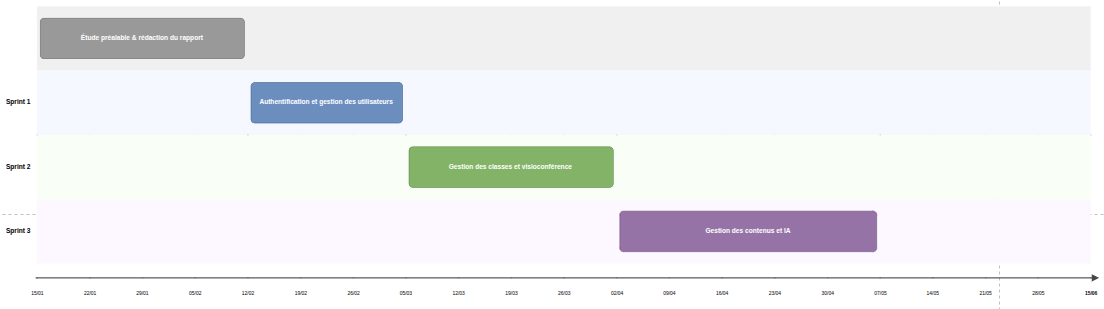
\includegraphics[width=\textwidth]{images/GANTT.png}
    \caption{Chronogramme de réalisation (Diagramme de Gantt)}
    \label{fig:gantt}
\end{figure}



% --- Section 3 : Modélisation ---
\section{Modélisation Sémantique et Comportementale}

La modélisation des besoins a pour objectif de transformer les exigences fonctionnelles en une représentation graphique claire des interactions entre les utilisateurs et le système. À cet effet, nous utilisons le \textbf{Diagramme de Cas d'Utilisation (Use Case Diagram)} issu du langage UML. 

Le diagramme présenté ci-dessous (voir Figure \ref{fig:use_case_global}) synthétise l'ensemble des interactions entre les trois acteurs du système et les fonctionnalités de la plateforme. Les trois acteurs héritent d'un acteur générique \textbf{Utilisateur} qui peut s'authentifier, gérer son profil et communiquer. Chaque acteur dispose de privilèges spécifiques :

\begin{itemize}
    \item \textbf{Administrateur :} Gère les utilisateurs (création, modification, suppression), les classes, les départements et les plannings.
    \item \textbf{Enseignant :} Gère les cours, les évaluations (manuelles ou par IA), les sessions vidéo via \textbf{Daily.co} et le suivi des présences.
    \item \textbf{Étudiant :} Consulte les cours, passe les évaluations et consulte sa progression.
\end{itemize}

\subsection{Diagramme de Cas d'Utilisation Global}

\newpage
\begin{figure}[ht!]
    \centering
    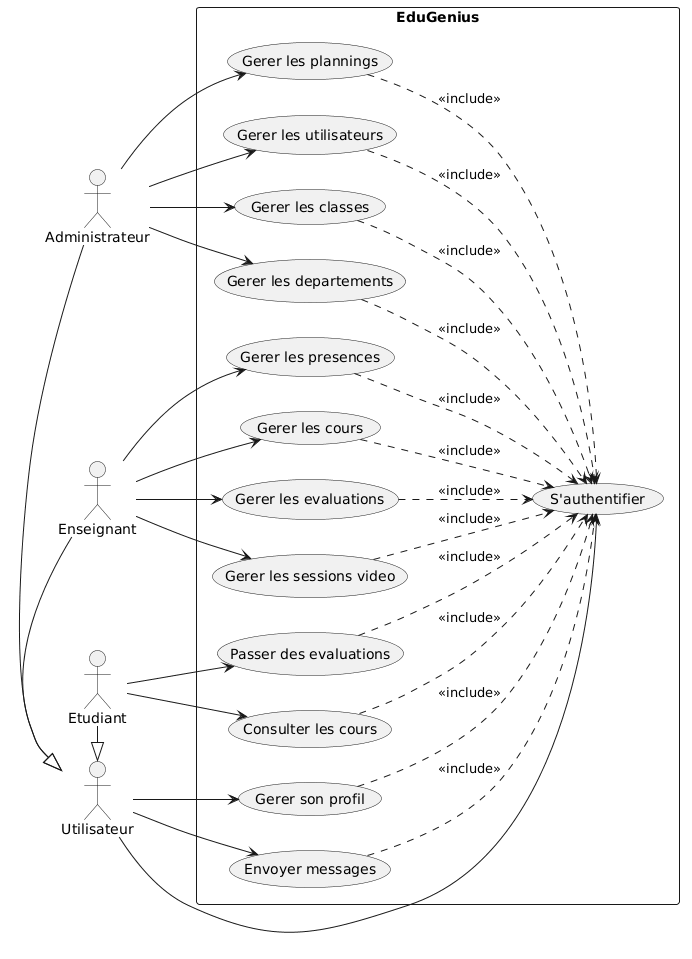
\includegraphics[width=0.85\textwidth, height=0.85\textheight, keepaspectratio]{images/use_case_global_diagram.png}
    \caption{Diagramme de cas d'utilisation global d'EduGenius}
    \label{fig:use_case_global}
\end{figure}

% --- Section 4 : Stack Technique ---
\section{Écosystème de Développement et Stack Technologique}

\subsection{Environnement de Collaboration}
Le succès du développement d'EduGenius repose sur une orchestration rigoureuse des outils de collaboration, permettant une gestion fluide du code source et du suivi de projet :

\begin{itemize}
    \item \textbf{GitHub :} Plateforme de forge logicielle utilisant Git pour le versionnement du code, facilitant le suivi des modifications et la sécurité des sources. \\ \begin{center} 
\includegraphics[width=3.5cm, height=1.2cm]{images/github_logo.png} \captionof{figure}{Logo GitHub} \end{center}
    \item \textbf{Trello :} Outil de gestion de projet basé sur la méthode Kanban, utilisé ici pour piloter le Product Backlog et l'avancement des Sprints Scrum. \\ \begin{center} 
\includegraphics[width=3.5cm, height=1.2cm]{images/trello_logo.png} \captionof{figure}{Logo Trello} \end{center}
    \item \textbf{Microsoft Teams :} Hub collaboratif utilisé pour centraliser les échanges, la documentation technique et les réunions de cadrage. \\ \begin{center} 
\includegraphics[width=3.5cm, height=1.2cm]{images/teams_logo.png} \captionof{figure}{Logo Microsoft Teams} \end{center}
\end{itemize}

\subsection{Stack Technologique : Le choix de la Performance}
L'architecture d'EduGenius repose sur une stack moderne, choisie pour sa capacité à gérer l'asynchronisme, la scalabilité et l'intégration de services temps réel :

\begin{itemize}
    \item \textbf{Next.js :} Framework full-stack basé sur React, utilisé pour le rendu hybride (SSR/SSG) et ses capacités de \textit{Server Actions}, optimisant ainsi la vitesse et le référencement \cite{nextjs_docs}. \\ \begin{center} 
\includegraphics[width=3.5cm, height=2.5cm, keepaspectratio]{images/next_logo.png} \captionof{figure}{Logo Next.js} \end{center}
    \item \textbf{Node.js \& Express :} Environnement d'exécution JavaScript côté serveur associé à un framework minimaliste pour la création d'API REST robustes et rapides \cite{learning_node}. \\ \begin{center} 
\includegraphics[width=3.5cm, height=1.2cm]{images/node_logo.png} \hspace{0.5cm} 
\includegraphics[width=3.5cm, height=1.2cm]{images/express_logo.png} \captionof{figure}{Logos Node.js et Express} \end{center}
    \item \textbf{MongoDB :} Base de données NoSQL orientée documents, offrant une grande flexibilité pour modéliser des structures de données éducatives évolutives \cite{mern_stack}. \\ \begin{center} 
\includegraphics[width=3.5cm, height=1.2cm]{images/mongodb_logo.png} \captionof{figure}{Logo MongoDB} \end{center}
    \item \textbf{AWS S3 :} Service de stockage d'objects cloud hautement disponible, utilisé pour l'hébergement sécurisé des supports de cours et fichiers multimédias. \\ \begin{center} 
\includegraphics[width=4cm, height=2cm]{images/s3_logo.png} \captionof{figure}{Logo AWS S3} \end{center}
    \item \textbf{Ollama :} Moteur d'inférence permettant l'exécution de modèles de langage (LLM) en local, garantissant la souveraineté et la confidentialité totale des données traitées \cite{generative_ai_survey}. \\ \begin{center} 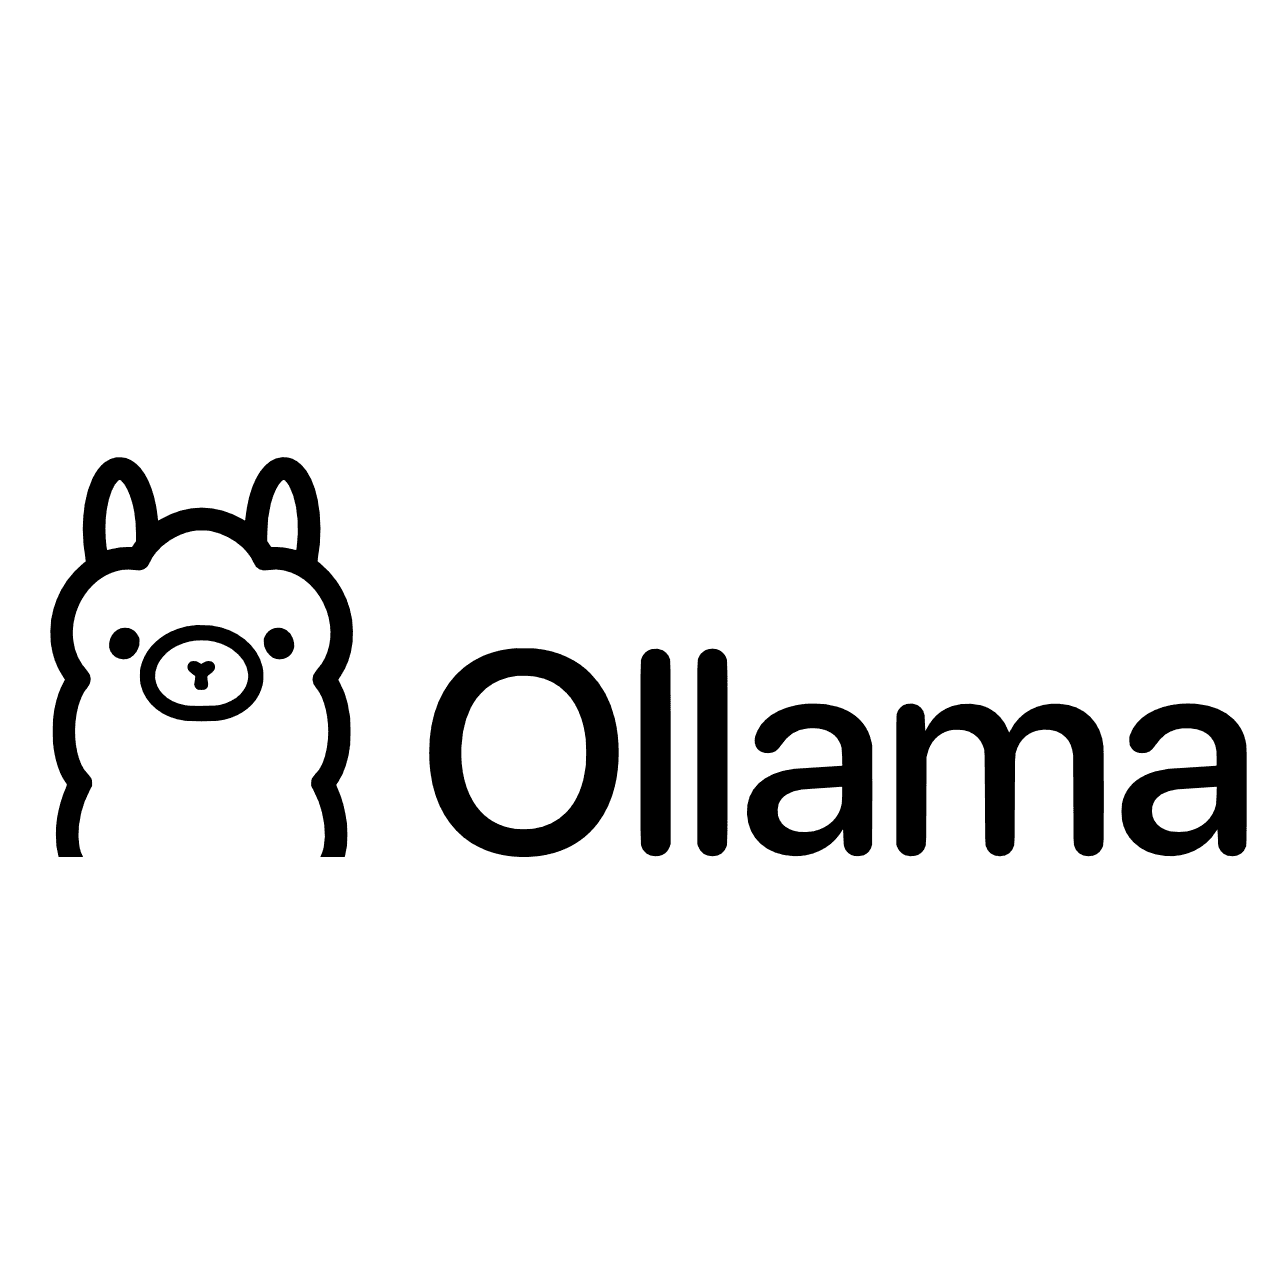
\includegraphics[width=3.5cm, height=3cm, keepaspectratio]{images/ollama_logo.png} \captionof{figure}{Logo Ollama} \end{center}
    \item \textbf{Daily.co :} API WebRTC spécialisée dans la vidéo haute définition, permettant l'intégration fluide des classes virtuelles directement dans l'interface \cite{webrtc_standard}. \\ \begin{center} 
\includegraphics[width=3.5cm, height=1.2cm]{images/daily_logo.png} \captionof{figure}{Logo Daily.co} \end{center}
    \item \textbf{Tailwind CSS :} Framework CSS utilitaire permettant une conception d'interface utilisateur rapide, moderne et entièrement responsive. \\ \begin{center} 
\includegraphics[width=3.5cm, height=2cm]{images/tailwind_logo.png} \captionof{figure}{Logo Tailwind CSS} \end{center}
    \item \textbf{Jest :} Framework de tests unitaires JavaScript, utilisé pour garantir la qualité du code et la non-régression des fonctionnalités métier par l'automatisation des tests. \\ \begin{center} 
\includegraphics[width=3.5cm, height=2cm, keepaspectratio]{images/jest.png} \captionof{figure}{Logo Jest} \end{center}
    \item \textbf{Postman :} Plateforme de collaboration pour le développement d'API, utilisée pour tester, simuler et documenter les endpoints REST du système de manière visuelle. \\ \begin{center} 
\includegraphics[width=3.5cm, height=2cm, keepaspectratio]{images/postman.png} \captionof{figure}{Logo Postman} \end{center}
    \item \textbf{Artillery :} Outil de test de charge et de performance moderne, utilisé pour simuler des flux d'utilisateurs intensifs et valider la scalabilité du système sous haute tension. \\ \begin{center} 
\includegraphics[width=4cm, height=2cm, keepaspectratio]{images/artillery_logo.png} \captionof{figure}{Logo Artillery} \end{center}
\end{itemize}

% --- Section 5 : Architecture ---
\section{Architecture Logicielle et Topologie Système}

L'architecture d'\textbf{EduGenius} a été conçue pour répondre à des impératifs de performance, de sécurité des données et de fluidité utilisateur. Elle repose sur une infrastructure hybride alliant services cloud et traitement local souverain, tout en respectant les principes de découplage de la \textit{Clean Architecture} \cite{clean_architecture}. Cette section détaille successivement l’organisation logique en couches puis la topologie matérielle et réseau.

\subsection{Architecture applicative (logique) : Modèle multi-tiers}

Le système adopte une architecture en couches (\textit{n-tier}), garantissant une séparation stricte des préoccupations (\textit{Separation of Concerns}) :

\begin{enumerate}
    \item \textbf{Couche de Présentation :} Développée avec \textbf{Next.js}, elle gère l'interface utilisateur, l'état applicatif et les interactions temps réel.
    \item \textbf{Couche Métier (Logic) :} Le serveur \textbf{Node.js} (Express) centralise la logique décisionnelle : orchestration de l'IA, gestion des sessions \textbf{Daily.co} et sécurité (JWT).
    \item \textbf{Couche d'Accès aux Données :} Interface avec \textbf{MongoDB} via l'ODM \textbf{Mongoose}, assurant la validation des schémas et l'intégrité des transactions.
\end{enumerate}

\subsection{Architecture physique (déploiement)}

La topologie de déploiement repose sur les composants suivants, interconnectés via les protocoles et flux représentés sur la figure \ref{fig:deployment_arch} :

\begin{itemize}
    \item \textbf{Clients :} Navigateurs web (desktop/mobile) communiquant en HTTPS/TLS 1.3 avec le serveur d’application.
    \item \textbf{Serveur d’application :} Instance VPS hébergeant les runtimes \textbf{Next.js} (rendu frontend) et \textbf{Express.js} (API REST). Il assure l’authentification JWT et orchestre les appels aux services externes.
    \item \textbf{Base de données :} Cluster \textbf{MongoDB Atlas} pour la persistance des utilisateurs, classes, cours, quiz et présences. La connexion s’effectue via l’ODM Mongoose.
    \item \textbf{Stockage objet :} Bucket \textbf{AWS S3} pour les fichiers volumineux (PDF, vidéos). L’accès se fait par URLs signées, soit directement par le client, soit via le backend.
    \item \textbf{Moteur IA local :} Serveur \textbf{Ollama} (modèle Gemma 3B) exécuté sur une machine dédiée, accessible via TCP/11434 en réseau interne. Toutes les données pédagogiques restent souveraines.
    \item \textbf{Service visioconférence :} \textbf{Daily.co} (cloud externe) est piloté en REST par l’application et fournit aux clients des flux WebRTC pour les classes virtuelles.
\end{itemize}

\begin{figure}[H]
    \centering
    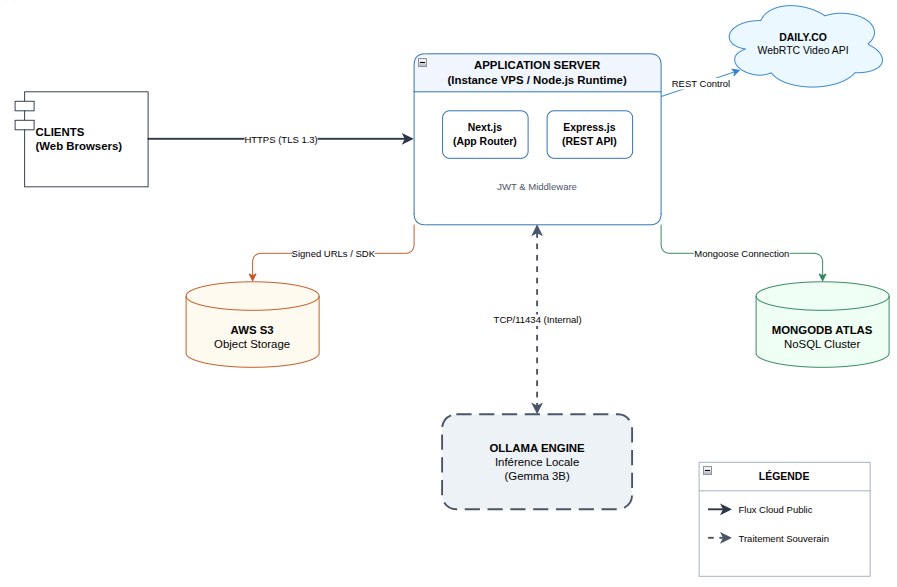
\includegraphics[width=\textwidth]{images/physical_architecture_diagram.png}
    \caption{Architecture de déploiement et flux d'infrastructure (physique)}
    \label{fig:deployment_arch}
\end{figure}

Cette infrastructure hybride garantit la scalabilité, la sécurité des données sensibles (traitement IA en local) et une expérience utilisateur fluide grâce à l’intégration native des services cloud.

% --- Conclusion du chapitre ---
\section*{Conclusion}
\addcontentsline{toc}{section}{Conclusion}

Ce chapitre a posé les bases conceptuelles et techniques du projet. L'analyse des besoins, la modélisation UML et les choix architecturaux retenus (Next.js, Express, MongoDB, Ollama, Daily.co) constituent un cadre solide pour les sprints de réalisation. Le chapitre suivant détaillera la mise en œuvre du Sprint 1, dédié à l'authentification et à la gestion des utilisateurs.
\chapter{Réalisation du Sprint 1 : Authentification et Gestion des Utilisateurs}

\section*{Introduction}
\addcontentsline{toc}{section}{Introduction}

Le premier sprint du projet EduGenius a été consacré à la mise en place du système d'authentification et des mécanismes de sécurité fondamentaux. Ces fonctionnalités constituent la pierre angulaire de la plateforme, visant à garantir la protection des données sensibles et à assurer un contrôle d'accès strict selon les rôles d'administrateur, d'enseignant et d'étudiant. Ce cycle de développement s'est structuré autour de plusieurs User Stories clés, couvrant notamment l'inscription des nouveaux membres, la connexion sécurisée via des protocoles modernes et la gestion de la récupération des comptes. 

Ce chapitre détaille l'ensemble des étapes ayant conduit à la concrétisation de ce premier incrément logiciel. Nous présenterons d'abord le backlog spécifique à ce sprint et l'analyse fonctionnelle des besoins identifiés. Ensuite, nous aborderons la conception technique et la réalisation des interfaces utilisateurs développées sous Next.js. Enfin, ce chapitre se conclura par une présentation des tests unitaires et d'intégration permettant de valider la robustesse et la fiabilité des fonctionnalités implémentées avant leur déploiement.


\section{Backlog du Sprint 1}

Le backlog du Sprint 1 présente les six User Stories (US) prioritaires liées à l'authentification, à la gestion des utilisateurs et aux fondations techniques (tableau de bord unifié et responsive). Ces US ont été sélectionnées pour leur impact métier et leur caractère transverse, structurant ainsi les développements clés de ce premier incrément.

Le tableau \ref{tab:sprint1_backlog} détaille chaque US avec ses critères d'acceptation et sa priorité. Les US-01 (Connexion sécurisée), US-02 (Gestion des rôles), US-04 (Création des classes), US-39 (Dashboard unifié) et US-41 (Interface responsive) sont classées comme « Haute » priorité en raison de leur rôle central dans la plateforme. L'US-03 (Profil utilisateur) est priorisée « Moyenne », car dépendante des précédentes mais non bloquante pour le reste du sprint. Les tâches techniques sous‑jacentes (chiffrement des mots de passe, génération de token JWT, adaptation CSS responsive) répondent aux exigences de sécurité et d'expérience utilisateur.

\begin{table}[H]
\centering
\small
\begin{tabularx}{\textwidth}{|c|l|X|c|}
\hline
\textbf{ID} & \textbf{Titre} & \textbf{Critères d’acceptation} & \textbf{Priorité} \\
\hline
US-01 & Connexion sécurisée & L'utilisateur peut se connecter avec les identifiants fournis par l'administrateur ; un token JWT valide est délivré. & Haute \\
\hline
US-02 & Gestion des rôles & L'administrateur peut attribuer les rôles (Admin, Enseignant, Étudiant) lors de la création ou modification d'un compte. & Haute \\
\hline
US-03 & Profil utilisateur & L'utilisateur peut consulter et modifier ses informations (nom, photo, mot de passe). & Moyenne \\
\hline
US-04 & Création et gestion des classes & L'administrateur peut créer, modifier ou supprimer une classe et y assigner des étudiants et un enseignant. & Haute \\
\hline
US-39 & Dashboard unifié & L'utilisateur dispose d'un tableau de bord personnalisé affichant son planning, les deadlines et les sessions à venir. & Haute \\
\hline
US-41 & Interface responsive & La plateforme est utilisable sur mobile, tablette et desktop sans perte de fonctionnalité. & Haute \\
\hline
\end{tabularx}
\caption{User Stories du Sprint 1 (Authentification et Sécurité)}
\label{tab:sprint1_backlog}
\end{table}

\section{Analyse}

\subsection{Diagramme de cas d’utilisation du Sprint 1}
Le diagramme de cas d’utilisation présenté en figure \ref{fig:usecase_sprint1} illustre les interactions entre l’utilisateur (non authentifié ou authentifié) et le système pour les fonctionnalités d’authentification et de gestion de profil.

\begin{figure}[H]
    \centering
    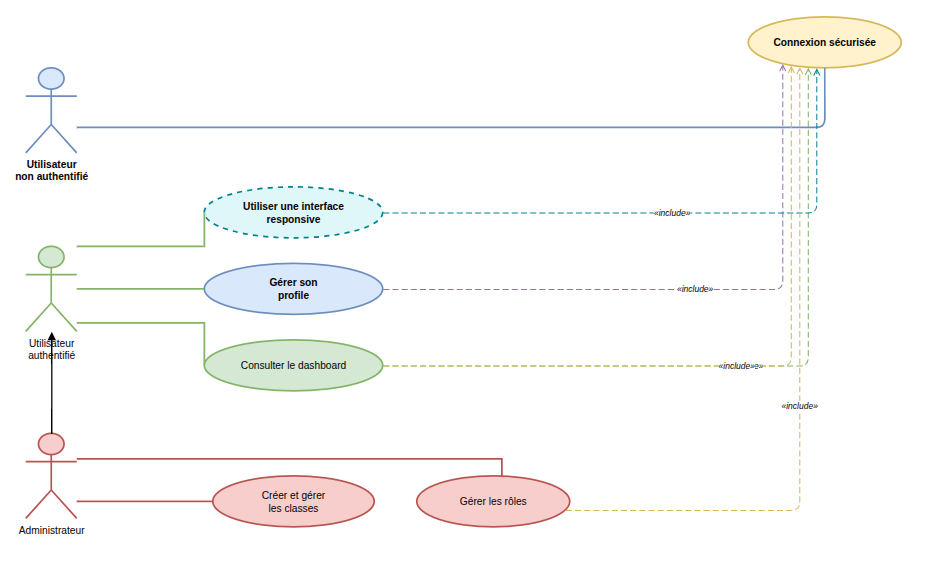
\includegraphics[width=1\textwidth]{images/sprint_1_usecase_diagram.png}
    \caption{Diagramme de cas d’utilisation – Authentification et sécurité}
    \label{fig:usecase_sprint1}
\end{figure}

\subsection{Description textuelle des cas d’utilisation}

Cette section décrit de manière structurée les scénarios nominaux et alternatifs pour chaque cas d'utilisation du sprint. Chaque cas (par exemple « S’authentifier ») est décomposé en éléments clés : acteur, préconditions, postconditions et étapes du scénario nominal. Le scénario nominal de connexion inclut la génération d’un token JWT, tandis qu’un échec (scénario alternatif) déclenche un message d’erreur générique. Les postconditions garantissent des états système cohérents, comme l’accès au tableau de bord après authentification.

\subsubsection{Le cas d’utilisation « S’authentifier »}
\begin{itemize}
    \item \textbf{Acteur} : Utilisateur non authentifié (futur élève, enseignant ou administrateur).
    \item \textbf{Préconditions} : Les comptes enseignants et étudiants ont été créés au préalable par l’administrateur ; le compte administrateur existe en base de données. L’utilisateur a reçu ses identifiants.
    \item \textbf{Postconditions} : Un token JWT valide est généré et l’utilisateur accède à son tableau de bord personnalisé.
    \item \textbf{Scénario nominal} :
    \begin{enumerate}
        \item L’utilisateur saisit son email et son mot de passe sur la page de connexion.
        \item Le système recherche l’utilisateur par email dans la collection MongoDB.
        \item Le système compare le mot de passe fourni avec le hachage bcrypt stocké.
        \item Le système génère un token JWT contenant l’identifiant, le rôle et la date d’expiration.
        \item Le token est retourné au client (cookie sécurisé / localStorage).
        \item L’utilisateur est redirigé vers son tableau de bord (adapté à son rôle).
    \end{enumerate}
    \item \textbf{Alternatives / Erreurs} :
    \begin{itemize}
        \item \textbf{Email inconnu ou mot de passe incorrect} : message générique « Identifiants invalides ».
        \item \textbf{Compte désactivé} : message invitant à contacter l’administrateur.
        \item \textbf{Token expiré} : l’utilisateur est invité à se reconnecter.
    \end{itemize}
\end{itemize}

\subsubsection{Le cas d’utilisation « Gérer son profil »}
\begin{itemize}
    \item \textbf{Acteur} : Utilisateur authentifié (élève, enseignant ou administrateur).
    \item \textbf{Préconditions} : L’utilisateur est connecté.
    \item \textbf{Postconditions} : Les informations modifiables (nom, photo, mot de passe) sont mises à jour en base.
    \item \textbf{Scénario nominal} :
    \begin{enumerate}
        \item L’utilisateur accède à la page « Mon profil ».
        \item Le système affiche les données actuelles.
        \item L’utilisateur modifie les champs autorisés et valide.
        \item Le système vérifie la validité des nouvelles données (unicité de l’email, complexité du mot de passe).
        \item Le système enregistre les modifications et affiche un message de confirmation.
    \end{enumerate}
    \item \textbf{Alternatives / Erreurs} :
    \begin{itemize}
        \item \textbf{Nouvel email déjà utilisé} : erreur et refus de la modification.
        \item \textbf{Mot de passe trop faible} : réaffichage des règles de sécurité.
    \end{itemize}
\end{itemize}

\subsubsection{Le cas d’utilisation « Consulter le tableau de bord »}
\begin{itemize}
    \item \textbf{Acteur} : Utilisateur authentifié.
    \item \textbf{Préconditions} : L’utilisateur est connecté.
    \item \textbf{Postconditions} : Le tableau de bord personnalisé est affiché (planning, notifications, évaluations à venir).
    \item \textbf{Scénario nominal} :
    \begin{enumerate}
        \item Après connexion ou en cliquant sur « Tableau de bord », le système agrège les données pertinentes.
        \item Pour un étudiant : affichage des cours à venir, devoirs, présences.
        \item Pour un enseignant : listes de ses classes, appels vidéo planifiés, quiz à corriger.
        \item Pour l’administrateur : statistiques générales, gestion des comptes.
    \end{enumerate}
    \item \textbf{Alternatives / Erreurs} :
    \begin{itemize}
        \item \textbf{Données non disponibles} : affichage de messages informatifs (ex. « Aucun cours planifié »).
    \end{itemize}
\end{itemize}

\subsubsection{Le cas d’utilisation « Utiliser l’interface responsive »}
\begin{itemize}
    \item \textbf{Acteur} : Tout utilisateur (non ou authentifié).
    \item \textbf{Préconditions} : L’utilisateur accède à la plateforme depuis un mobile, une tablette ou un ordinateur.
    \item \textbf{Postconditions} : La mise en page s’adapte automatiquement à la taille de l’écran sans perte de fonctionnalité.
    \item \textbf{Scénario nominal} :
    \begin{enumerate}
        \item L’utilisateur ouvre l’application sur un smartphone.
        \item Les styles CSS réorganisent les éléments (menu en accordéon, polices lisibles).
        \item Toutes les actions (connexion, consultation de cours, quiz) restent accessibles.
    \end{enumerate}
    \item \textbf{Alternatives / Erreurs} :
    \begin{itemize}
        \item \textbf{Navigation dégradée} : si une fonctionnalité n’est pas adaptée, un message invite à passer sur un écran plus large.
    \end{itemize}
\end{itemize}

\subsubsection{Le cas d’utilisation « Gérer les utilisateurs » (administrateur)}
\begin{itemize}
    \item \textbf{Acteur} : Administrateur.
    \item \textbf{Préconditions} : L’administrateur est connecté.
    \item \textbf{Postconditions} : Un compte enseignant ou étudiant est créé (ou modifié/supprimé) dans la collection \texttt{User}.
    \item \textbf{Scénario nominal (création)} :
    \begin{enumerate}
        \item L’administrateur accède à l’interface « Gestion des utilisateurs ».
        \item Il clique sur « Ajouter un utilisateur » et remplit le formulaire (nom, prénom, email, rôle enseignant/étudiant).
        \item Le système vérifie l’unicité de l’email et la validité des champs.
        \item Le système génère un mot de passe temporaire sécurisé, le hache et enregistre l’utilisateur.
        \item Un email contenant les identifiants (email + mot de passe temporaire) est envoyé à l’utilisateur.
        \item L’utilisateur devra changer son mot de passe lors de la première connexion.
    \end{enumerate}
    \item \textbf{Alternatives / Erreurs} :
    \begin{itemize}
        \item \textbf{Email déjà existant} : refus de création, message d’erreur.
        \item \textbf{Rôle invalide} : l’administrateur ne peut pas créer un autre administrateur via cette interface (réservé à une procédure manuelle).
    \end{itemize}
\end{itemize}

\subsubsection{Le cas d’utilisation « Créer et gérer les classes » (administrateur)}
\begin{itemize}
    \item \textbf{Acteur} : Administrateur.
    \item \textbf{Préconditions} : L’administrateur est connecté. Les départements, programmes et années académiques existent.
    \item \textbf{Postconditions} : Une classe est créée, modifiée ou supprimée, avec assignation d’un enseignant et d’étudiants.
    \item \textbf{Scénario nominal} :
    \begin{enumerate}
        \item L’administrateur remplit le formulaire de création (nom, code, département, programme, année).
        \item Il sélectionne les étudiants inscrits et l’enseignant responsable.
        \item Le système ajoute la classe dans MongoDB et met à jour les références.
    \end{enumerate}
    \item \textbf{Alternatives / Erreurs} :
    \begin{itemize}
        \item \textbf{Code de classe déjà existant} : message d’erreur demandant un autre code.
        \item \textbf{Suppression d’une classe contenant des cours actifs} : confirmation requise.
    \end{itemize}
\end{itemize}
\begin{itemize}
    \item \textbf{Acteur} : Utilisateur authentifié (étudiant, enseignant ou admin).
    \item \textbf{Préconditions} : L’utilisateur est connecté.
    \item \textbf{Postconditions} : Les informations du profil sont mises à jour selon les modifications demandées.
    \item \textbf{Scénario nominal (consultation)} :
    \begin{enumerate}
        \item L’utilisateur accède à son espace « Mon profil ».
        \item Le système affiche les informations actuelles (nom, prénom, email, photo, etc.).
    \end{enumerate}
    \item \textbf{Scénario nominal (modification)} :
    \begin{enumerate}
        \item L’utilisateur modifie un ou plusieurs champs modifiables (nom, photo, mot de passe).
        \item Le système valide les nouvelles données (format, unicité de l’email si modifié).
        \item Le système enregistre les changements.
        \item Un message de confirmation est affiché.
    \end{enumerate}
    \item \textbf{Alternatives / Erreurs} :
    \begin{itemize}
        \item \textbf{Nouvel email déjà utilisé} : erreur et refus de la modification.
        \item \textbf{Nouveau mot de passe trop faible} : le système exige des critères de robustesse.
    \end{itemize}
\end{itemize}

\section{Conception}
\subsection{Diagramme de séquence du cas « S’authentifier »}
\begin{figure}[H]
    \centering
    % \includegraphics[width=0.8\textwidth]{images/sequence_auth.png}
    \caption{Diagramme de séquence de l’authentification JWT}
    \label{fig:sequence_auth}
\end{figure}

\subsection{Diagramme de séquence du cas « Consulter profil »}
\begin{figure}[H]
    \centering
    % \includegraphics[width=0.8\textwidth]{images/sequence_profil.png}
    \caption{Diagramme de séquence de la consultation du profil}
    \label{fig:sequence_profil}
\end{figure}

\subsection{Diagramme de classes du Sprint 1}
\begin{figure}[H]
    \centering
    % \includegraphics[width=\textwidth]{images/class_sprint1.png}
    \caption{Diagramme de classes – Modèle utilisateur et authentification}
    \label{fig:class_sprint1}
\end{figure}

\subsection{Représentation graphique de la base de données}
\begin{figure}[H]
    \centering
    % \includegraphics[width=\textwidth]{images/mongodb_sprint1.png}
    \caption{Schéma des collections MongoDB pour le sprint 1}
    \label{fig:mongodb_sprint1}
\end{figure}

\section{Réalisation}
\subsection{Interface d’inscription}
\begin{figure}[H]
    \centering
    % \includegraphics[width=0.7\textwidth]{images/register_ui.png}
    \caption{Formulaire d’inscription}
    \label{fig:register_ui}
\end{figure}

\subsection{Interface de connexion}
\begin{figure}[H]
    \centering
    % \includegraphics[width=0.7\textwidth]{images/login_ui.png}
    \caption{Page de connexion}
    \label{fig:login_ui}
\end{figure}

\subsection{Interface de réinitialisation de mot de passe}
\begin{figure}[H]
    \centering
    % \includegraphics[width=0.7\textwidth]{images/reset_ui.png}
    \caption{Formulaire de réinitialisation}
    \label{fig:reset_ui}
\end{figure}

\subsection{Interface profil utilisateur}
\begin{figure}[H]
    \centering
    % 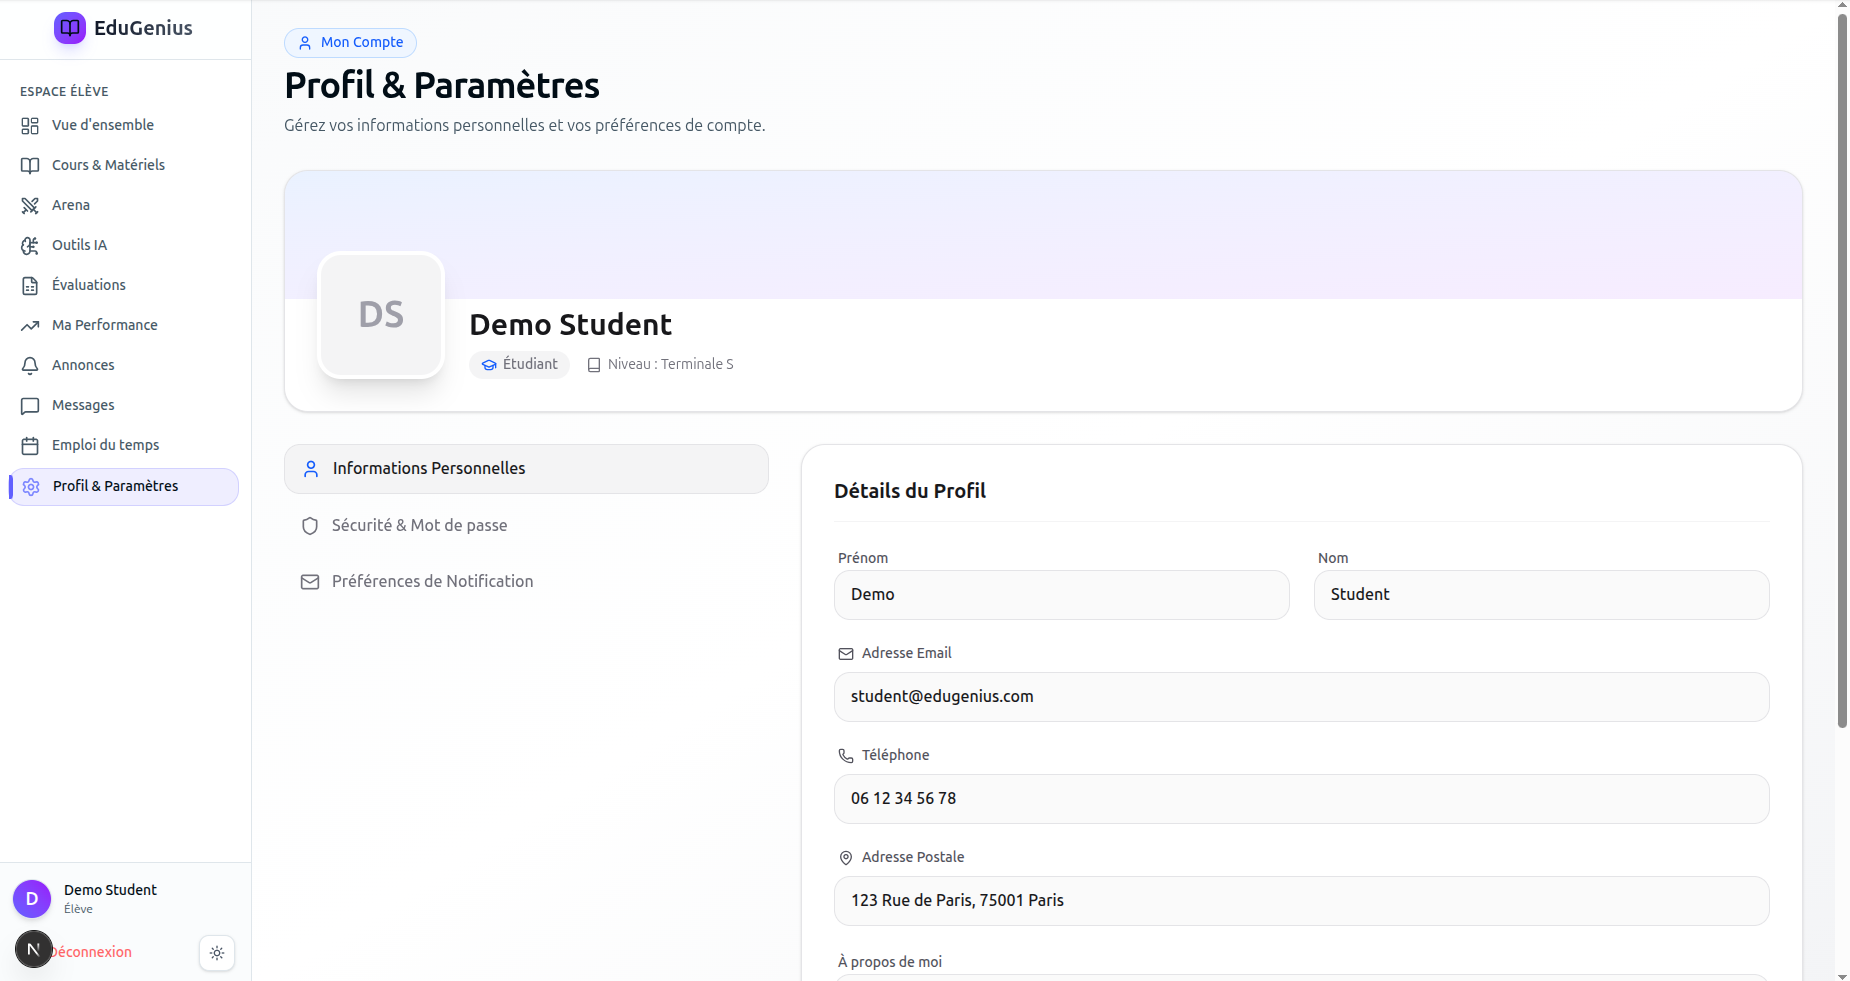
\includegraphics[width=0.7\textwidth]{images/profile_ui.png}
    \caption{Page de profil}
    \label{fig:profile_ui}
\end{figure}

\section{Tests}
\subsection{Tests unitaires}
\ldots

\subsection{Tests d’intégration}
\ldots

\subsection{Tests fonctionnels}
\ldots

\section{Conclusion}
\ldots
\chapter{Réalisation du Sprint 2 : Gestion des classes et visio-conférence}

\section*{Introduction}
\addcontentsline{toc}{section}{Introduction}

Le deuxième sprint du projet a été consacré à la mise en place des fonctionnalités de gestion des classes, de la planification et de la communication synchrone. Ces fonctionnalités sont essentielles pour permettre aux utilisateurs de structurer l'organisation pédagogique, de collaborer en direct via visioconférence et de superviser le déroulement des enseignements.

Ce chapitre présente les étapes du développement de ce sprint : le backlog, l'analyse fonctionnelle, la conception, la réalisation des interfaces et les tests associés.

\section{Backlog du Sprint 2}

Le backlog du Sprint 2 compile onze User Stories couvrant la gestion des classes et des plannings, ainsi que la création, le suivi, la modération et l’enregistrement des appels vidéo. Ces US ont été priorisées « Haute », « Moyenne » ou « Basse » selon leur criticité pour la continuité pédagogique. Le tableau \ref{tab:sprint2_backlog} détaille chaque US avec ses critères d’acceptation.

\begin{xltabular}{\textwidth}{|c|>{\raggedright\arraybackslash}p{4cm}|X|c|}
\hline
\textbf{ID} & \textbf{Titre} & \textbf{Critères d’acceptation} & \textbf{Priorité} \\
\hline
\endfirsthead

\multicolumn{4}{c}{{\bfseries \tablename\ \thetable{} -- suite de la page précédente}} \\
\hline
\textbf{ID} & \textbf{Titre} & \textbf{Critères d’acceptation} & \textbf{Priorité} \\
\hline
\endhead

\hline
\multicolumn{4}{|r|}{\textit{Suite sur page suivante}} \\
\endfoot

\hline
\caption{User Stories du Sprint 2 – Gestion des classes et visioconférence} \label{tab:sprint2_backlog}
\endlastfoot

US-06 & Création et gestion des classes & L’administrateur peut créer, modifier, supprimer des classes et y assigner des étudiants et un enseignant. & Haute \\
\hline
US-07 & Planification des cours & L’administrateur définit les horaires des classes (date, heure, durée) dans un emploi du temps interactif. & Haute \\
\hline
US-08 & Supervision générale & L’administrateur dispose d'une vue d'ensemble sur les utilisateurs, les classes et les activités récentes. & Moyenne \\
\hline
US-09 & Création d’un appel vidéo & L’enseignant peut démarrer une session Daily.co directement depuis le planning. & Haute \\
\hline
US-10 & Rejoindre un appel vidéo & L’étudiant rejoint la session vidéo prévue en un clic depuis son tableau de bord. & Haute \\
\hline
US-11 & Partage d’écran & L’enseignant peut partager son écran (présentation, code) avec l'ensemble des participants. & Haute \\
\hline
US-12 & Modération audio/vidéo & L’enseignant peut couper le micro ou la caméra d’un étudiant pour maintenir le calme. & Moyenne \\
\hline
US-13 & Chat de session & Les participants peuvent échanger des messages textuels en temps réel pendant l'appel vidéo. & Moyenne \\
\hline
US-14 & Détection de présence & Le système enregistre automatiquement l'heure d'arrivée, les retards et les absences des étudiants. & Haute \\
\hline
US-15 & Historique de participation & L’enseignant et l'admin peuvent consulter l’historique des présences détaillé par séance. & Haute \\
\hline
US-16 & Enregistrement et replay & Les sessions peuvent être enregistrées et consultées ultérieurement par les étudiants. & Basse \\
\hline
\end{xltabular}

\section{Analyse}

\subsection{Diagramme de cas d’utilisation du Sprint 2}
Le diagramme de cas d’utilisation (figure \ref{fig:usecase_sprint2}) illustre les interactions entre l’administrateur, l’enseignant et l’étudiant pour la gestion des classes, la planification, les notifications, les appels vidéo avec modération, chat intégré et replay.

\begin{figure}[H]
    \centering
    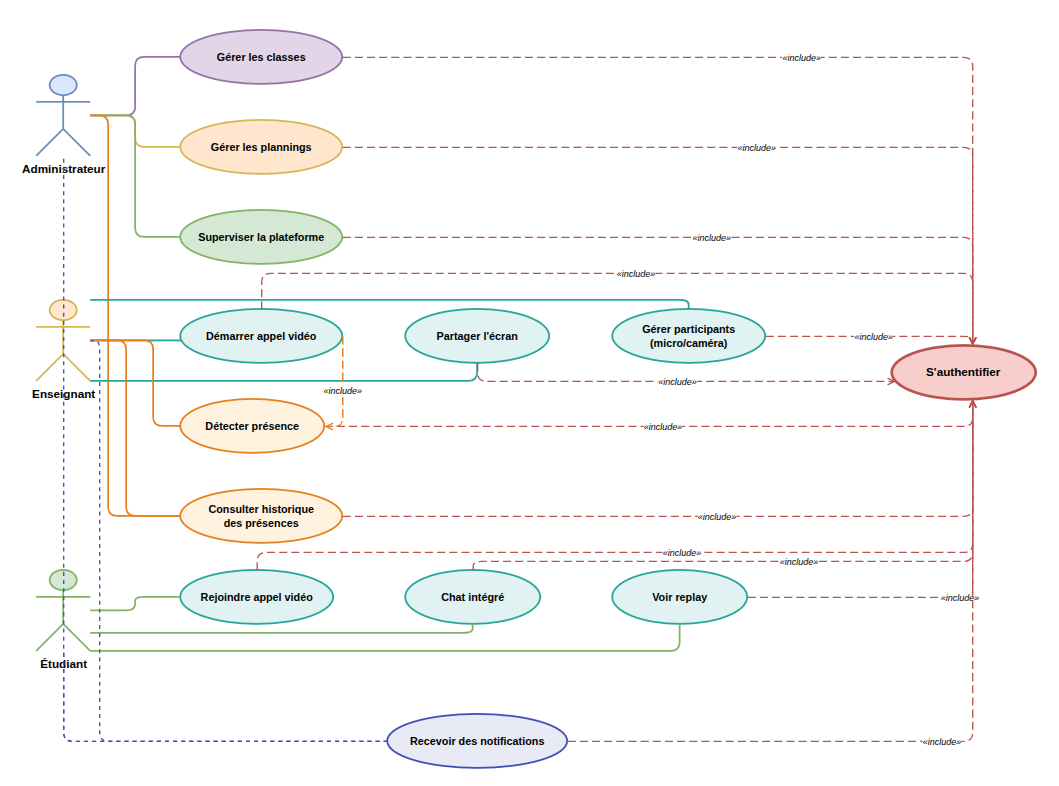
\includegraphics[width=1\textwidth]{images/use_case_diagram_sprint_2.png}
    \caption{Diagramme de cas d’utilisation – Gestion des
classes et visioconférence}
    \label{fig:usecase_sprint2}
\end{figure}

\subsection{Description textuelle des cas d’utilisation}
Cette section détaille de manière structurée les scénarios nominaux et alternatifs pour chaque cas d’utilisation clé du second sprint. Les descriptions suivent un format standardisé pour garantir une compréhension claire des interactions système et des règles métier associées.

\subsection{Cas d'utilisation : Créer une classe}
Ce cas permet à l'administrateur de créer un nouveau groupe pédagogique en définissant ses caractéristiques et son rattachement.

\begin{table}[H]
\centering
\small
\begin{tabularx}{\textwidth}{|l|X|}
\hline
\rowcolor[HTML]{EFEFEF} 
\textbf{Acteur(s)} & Administrateur \\ \hline
\textbf{Pré-conditions} & L'admin doit être authentifié et les départements doivent être configurés. \\ \hline
\textbf{Post-conditions} & La classe est créée et prête à recevoir un emploi du temps. \\ \hline
\textbf{Scénario nominal} & 
1. L'admin accède au module de création de classes. \newline
2. Il saisit les informations (Nom, Code, Année, Niveau). \newline
3. Il sélectionne le département de rattachement. \newline
4. Le système valide et persiste les données. \newline
5. La classe apparaît dans la liste des classes. \\ \hline
\textbf{Scénario alternatif} & 
2.a. Code classe existant : le système affiche une erreur de duplication. \\ \hline
\end{tabularx}
\caption{Description textuelle - Créer une classe}
\end{table}

\subsection{Cas d'utilisation : Créer un emploi du temps}
Ce cas permet à l'administrateur de définir les créneaux horaires des enseignements pour une classe donnée.

\begin{table}[H]
\centering
\small
\begin{tabularx}{\textwidth}{|l|X|}
\hline
\rowcolor[HTML]{EFEFEF} 
\textbf{Acteur(s)} & Administrateur \\ \hline
\textbf{Pré-conditions} & La classe, les matières et les enseignants doivent exister. \\ \hline
\textbf{Post-conditions} & L'emploi du temps est créé et visible par les acteurs concernés. \\ \hline
\textbf{Scénario nominal} & 
1. L'admin sélectionne une classe cible. \newline
2. Il ajoute une séance (Jour, Heure, Matière, Enseignant). \newline
3. Le système vérifie la disponibilité de l'enseignant. \newline
4. L'admin valide le planning hebdomadaire. \newline
5. L'emploi du temps est publié. \\ \hline
\textbf{Scénario alternatif} & 
3.a. Conflit d'horaire : le système signale que l'enseignant est déjà occupé sur ce créneau. \\ \hline
\end{tabularx}
\caption{Description textuelle - Créer un emploi du temps}
\end{table}

\subsection{Cas d'utilisation : Gérer l'assiduité}
Le système assure de manière autonome le suivi de la présence des étudiants lors des sessions de visioconférence.

\begin{table}[H]
\centering
\small
\begin{tabularx}{\textwidth}{|l|X|}
\hline
\rowcolor[HTML]{EFEFEF} 
\textbf{Acteur(s)} & Système \\ \hline
\textbf{Pré-conditions} & Une séance virtuelle doit être en cours. \\ \hline
\textbf{Post-conditions} & Les journaux de présence sont mis à jour en base de données. \\ \hline
\textbf{Scénario nominal} & 
1. Le système détecte l'entrée d'un étudiant dans la salle virtuelle. \newline
2. Il enregistre l'horodatage exact de connexion. \newline
3. Il surveille la durée totale de participation. \newline
4. Il génère le statut (Présent/Retard/Absent) à la fin de la séance. \\ \hline
\textbf{Scénario alternatif} & 
1.a. Déconnexion/Reconnexion : le système cumule les temps de présence fragmentés. \\ \hline
\end{tabularx}
\caption{Description textuelle - Gérer l'assiduité}
\end{table}

\subsection{Cas d'utilisation : Consulter les Replays}
Les utilisateurs accèdent aux archives vidéo des séances passées pour révision ou rattrapage.

\begin{table}[H]
\centering
\small
\begin{tabularx}{\textwidth}{|l|X|}
\hline
\rowcolor[HTML]{EFEFEF} 
\textbf{Acteur(s)} & Enseignant, Étudiant \\ \hline
\textbf{Pré-conditions} & La séance doit avoir été enregistrée et le flux traité. \\ \hline
\textbf{Post-conditions} & La vidéo est visionnée dans le lecteur intégré. \\ \hline
\textbf{Scénario nominal} & 
1. L'utilisateur accède à la médiathèque de sa classe. \newline
2. Il sélectionne une séance archivée. \newline
3. Le système récupère le flux depuis le stockage Cloud. \newline
4. Le lecteur multimédia démarre la lecture. \\ \hline
\textbf{Scénario alternatif} & 
3.a. Fichier non disponible : le système indique que le replay est en cours de traitement. \\ \hline
\end{tabularx}
\caption{Description textuelle - Consulter les Replays}
\end{table}

\section{Conception}

\subsection{Diagramme de séquence du cas : Créer une classe}
Le diagramme de séquence de la figure \ref{fig:create_class_sequence} détaille le processus administratif de structuration d'un groupe pédagogique. Ce flux illustre la coordination entre l'interface de gestion, le service d'API et la persistance en base de données. L'administrateur définit les paramètres de la classe (nom, département, niveau) et le système assure l'intégrité référentielle en liant ces entités dans la collection MongoDB, garantissant ainsi un socle solide pour la planification ultérieure des cours.

\begin{figure}[H]
    \centering
    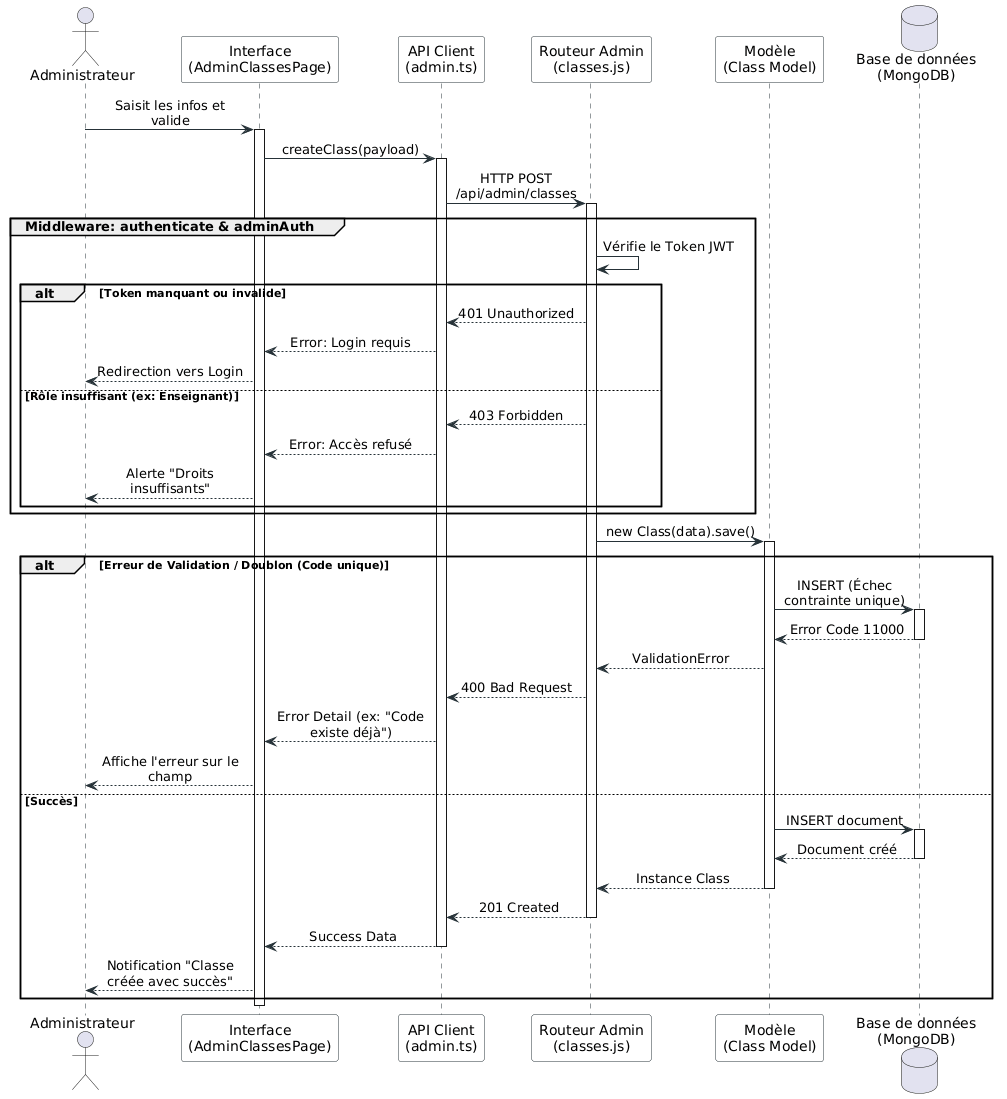
\includegraphics[width=\textwidth]{images/class_management_sequence_diagram.png}
    \caption{Diagramme de séquence – Création et configuration d'une classe (Admin)}
    \label{fig:create_class_sequence}
\end{figure}

\subsection{Diagramme de séquence du cas : Rejoindre une séance et détection de présence}
La figure \ref{fig:presence_sequence} expose le mécanisme complexe de communication synchrone et de suivi automatisé. Lorsqu'un utilisateur rejoint une salle virtuelle, le frontend initialise le SDK \textbf{Daily.co} pour établir le flux WebRTC. Simultanément, un événement de connexion déclenche un appel asynchrone vers le backend. Le système identifie l'utilisateur via son token JWT et enregistre automatiquement son horodatage d'entrée. Ce processus transparent garantit la fiabilité des relevés d'assiduité sans intervention manuelle de l'enseignant.

\begin{figure}[H]
    \centering
    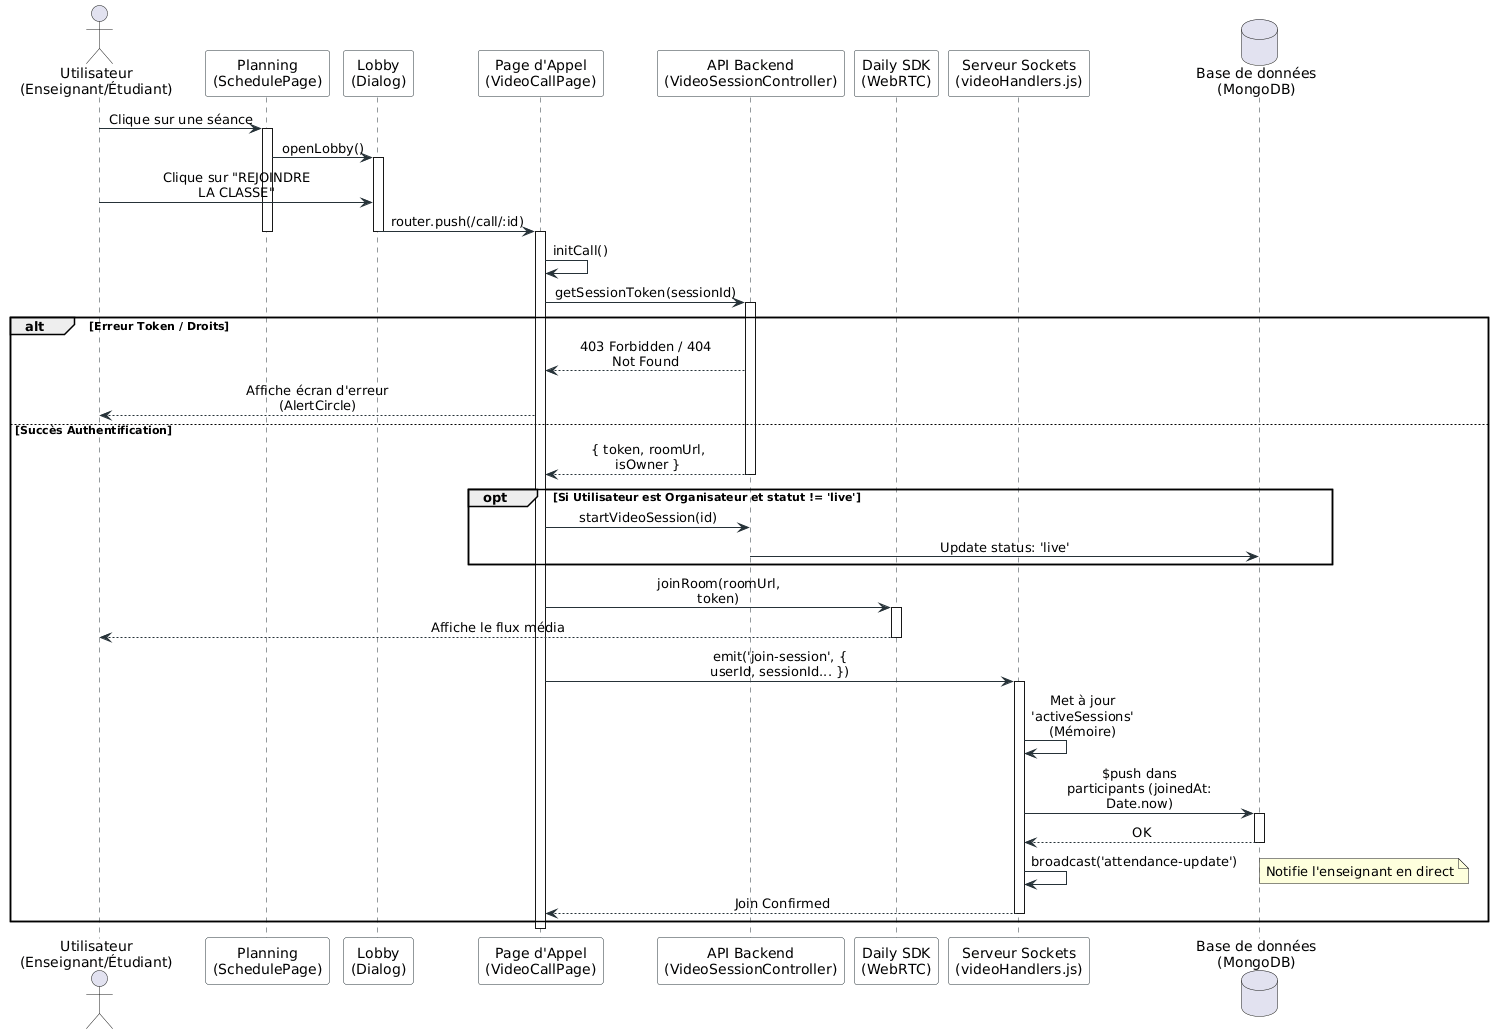
\includegraphics[width=\textwidth]{images/join_call_sequence_diagram.png}
    \caption{Diagramme de séquence – Accès à la visioconférence et suivi de présence automatique}
    \label{fig:presence_sequence}
\end{figure}

\subsection{Diagramme de classes du Sprint 2}
La figure \ref{fig:class_sprint2} présente le modèle structurel du second sprint, centré sur la gestion des classes et la communication synchrone. L'entité centrale \texttt{Class} s'enrichit de méthodes de gestion des effectifs (\texttt{joinClass}, \texttt{assignTeacher}). La planification est assurée par le modèle \texttt{Schedule} et ses entrées détaillées (\texttt{ScheduleEntry}). Le cœur de la visioconférence repose sur \texttt{VideoSession}, qui orchestre les interactions avec l'API Daily.co et génère, à sa clôture, une entité \texttt{Attendance}. Ce diagramme met également en évidence l'intégration des profils \texttt{Teacher} et \texttt{Student} au sein de l'objet \texttt{User}, assurant une spécialisation des données sans complexifier l'héritage en base.

\begin{figure}[H]
    \centering
    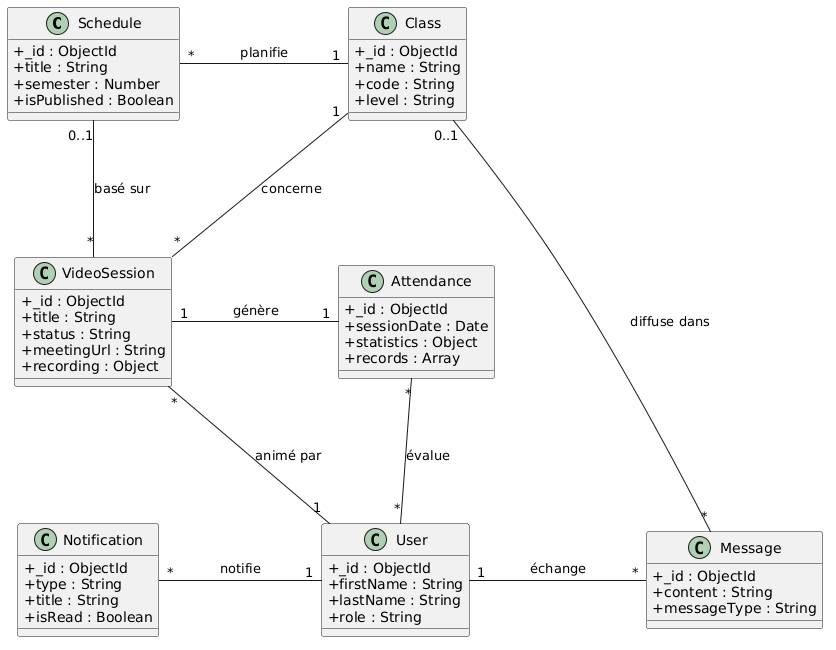
\includegraphics[width=\textwidth]{images/class_diagram_sprint_2.png}
    \caption{Diagramme de classes – Gestion des classes, sessions vidéo et suivi d'assiduité}
    \label{fig:class_sprint2}
\end{figure}

\subsection{Représentation graphique de la base de données}
Le schéma physique de la base de données (figure \ref{fig:mongodb_sprint2}) illustre la transition d'EduGenius vers un système de gestion pédagogique complet. L'architecture NoSQL a été optimisée pour supporter des requêtes complexes sur les emplois du temps et les statistiques de présence.

La collection \texttt{classes} agit comme le pivot organisationnel, liant les départements aux utilisateurs. Elle stocke de manière atomique les tableaux d'enseignants et d'étudiants, facilitant ainsi les contrôles d'accès lors des sessions live. La gestion temporelle est déléguée à la collection \texttt{schedules}, dont la structure par entrées permet de définir des cycles hebdomadaires récurrents.

Le suivi de la communication synchrone repose sur un couplage fort entre \texttt{videosessions} et \texttt{attendances}. Tandis que la première conserve les métadonnées techniques de l'appel (URLs, jetons Daily.co, paramètres de modération), la seconde centralise les rapports d'assiduité calculés. Cette séparation permet de purger les logs techniques de session tout en conservant l'historique pédagogique des présences, optimisant ainsi l'espace de stockage sur le long terme.

\begin{figure}[H]
    \centering
    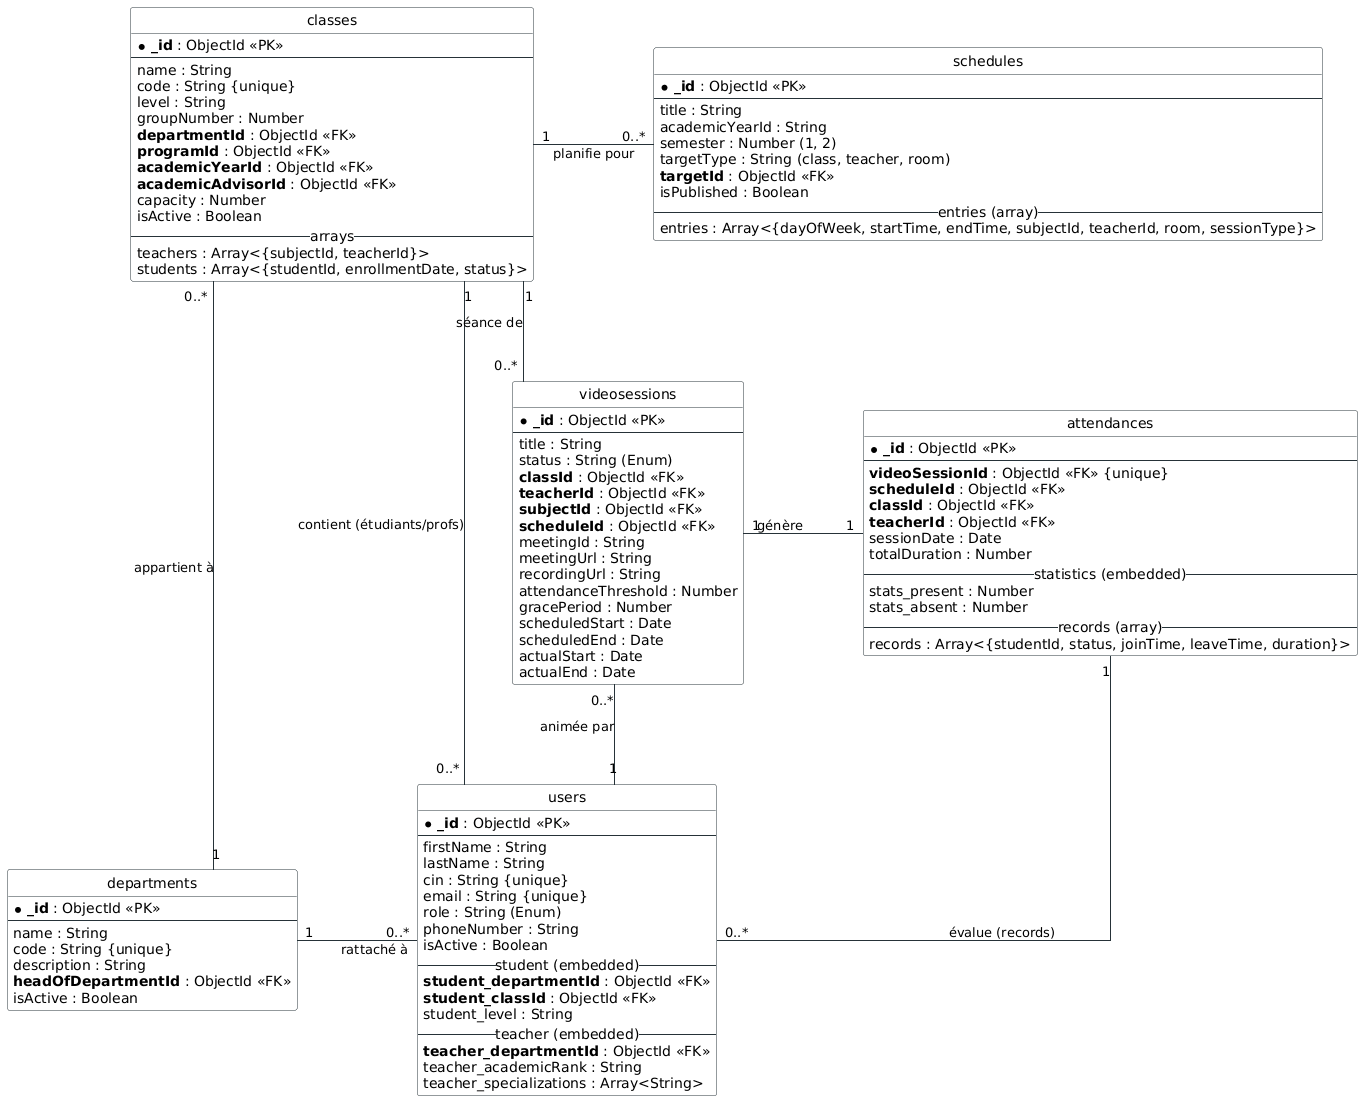
\includegraphics[width=\textwidth]{images/ERD_sprint_2.png}
    \caption{Schéma des collections MongoDB pour le sprint 2}
    \label{fig:mongodb_sprint2}
\end{figure}

\section{Réalisation}

\subsection{Interface de gestion des classes (Admin)}

L'interface de gestion des classes présente une vue en cartes avec les informations clés (nom, code, département, niveau, effectif). L'administrateur peut créer, modifier ou désactiver une classe, inscrire des étudiants via une recherche avec sélection multiple, et assigner des enseignants par matière dans une modale dédiée.

\begin{figure}[H]
    \centering
    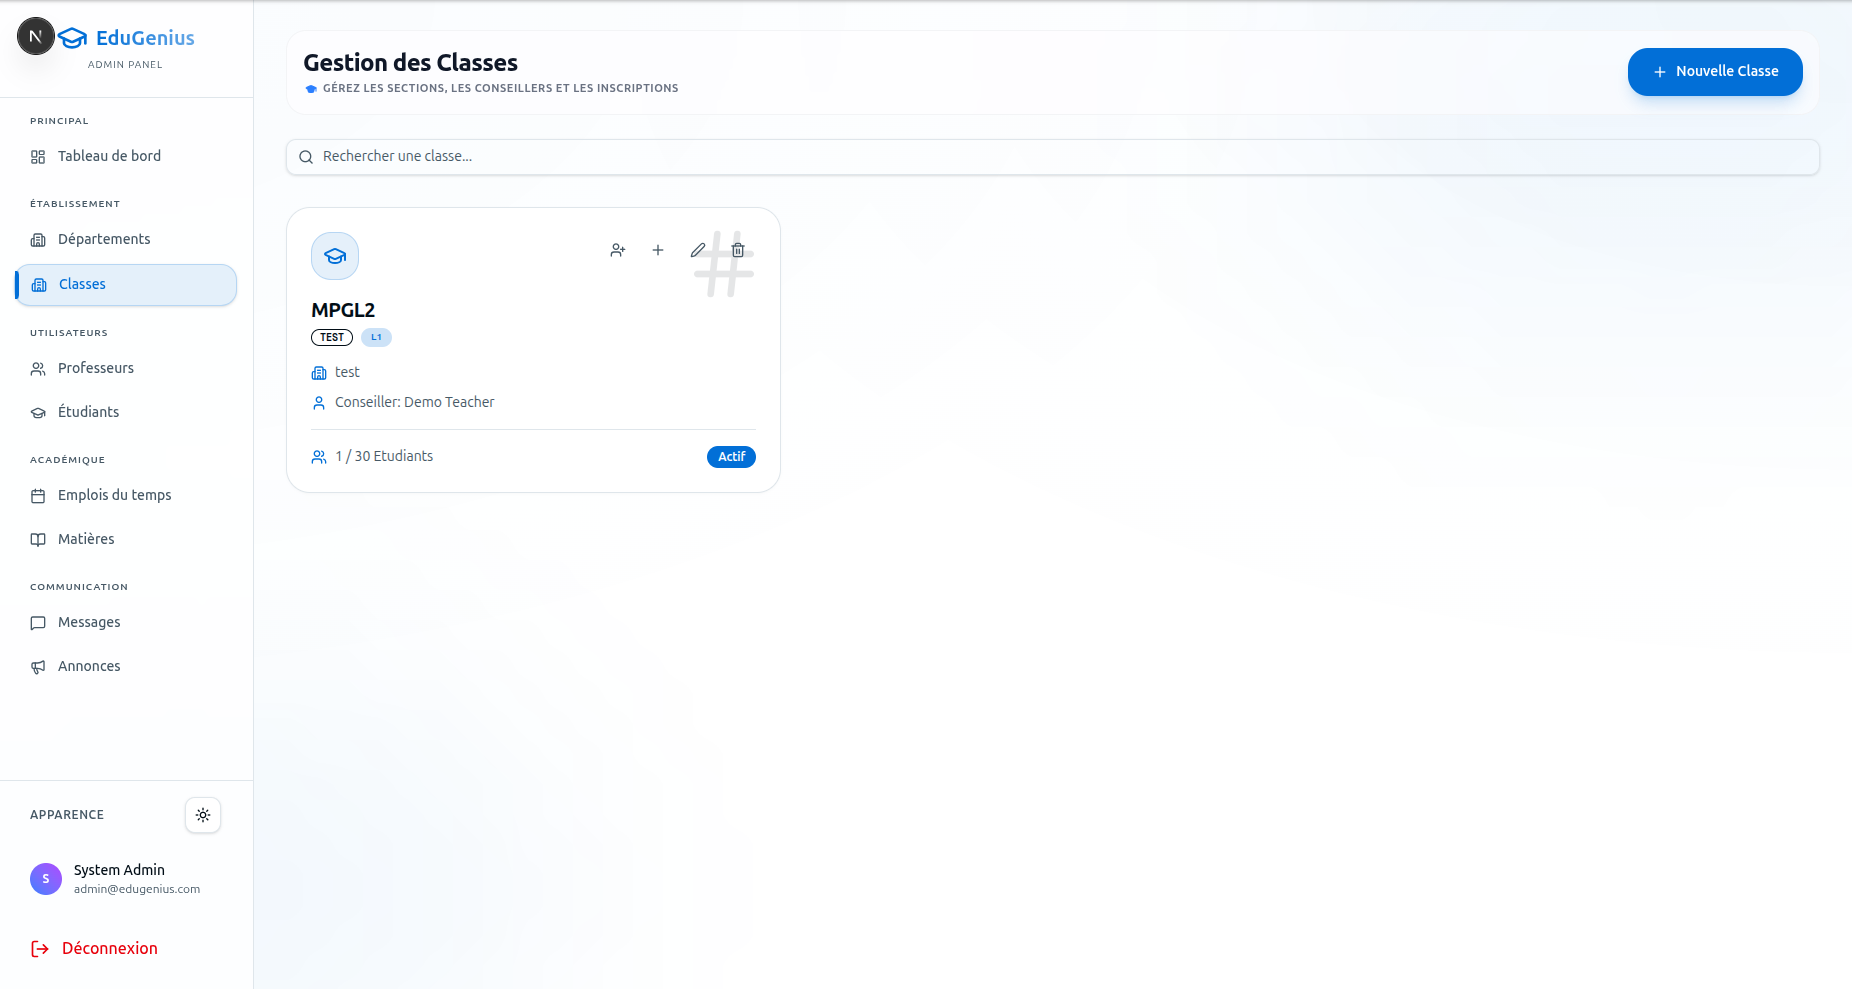
\includegraphics[width=\textwidth]{images/class_management_ui_1.png}
    \caption{Interface de gestion des classes : Liste générale}
    \label{fig:class_list_ui}
\end{figure}

\begin{figure}[H]
    \centering
    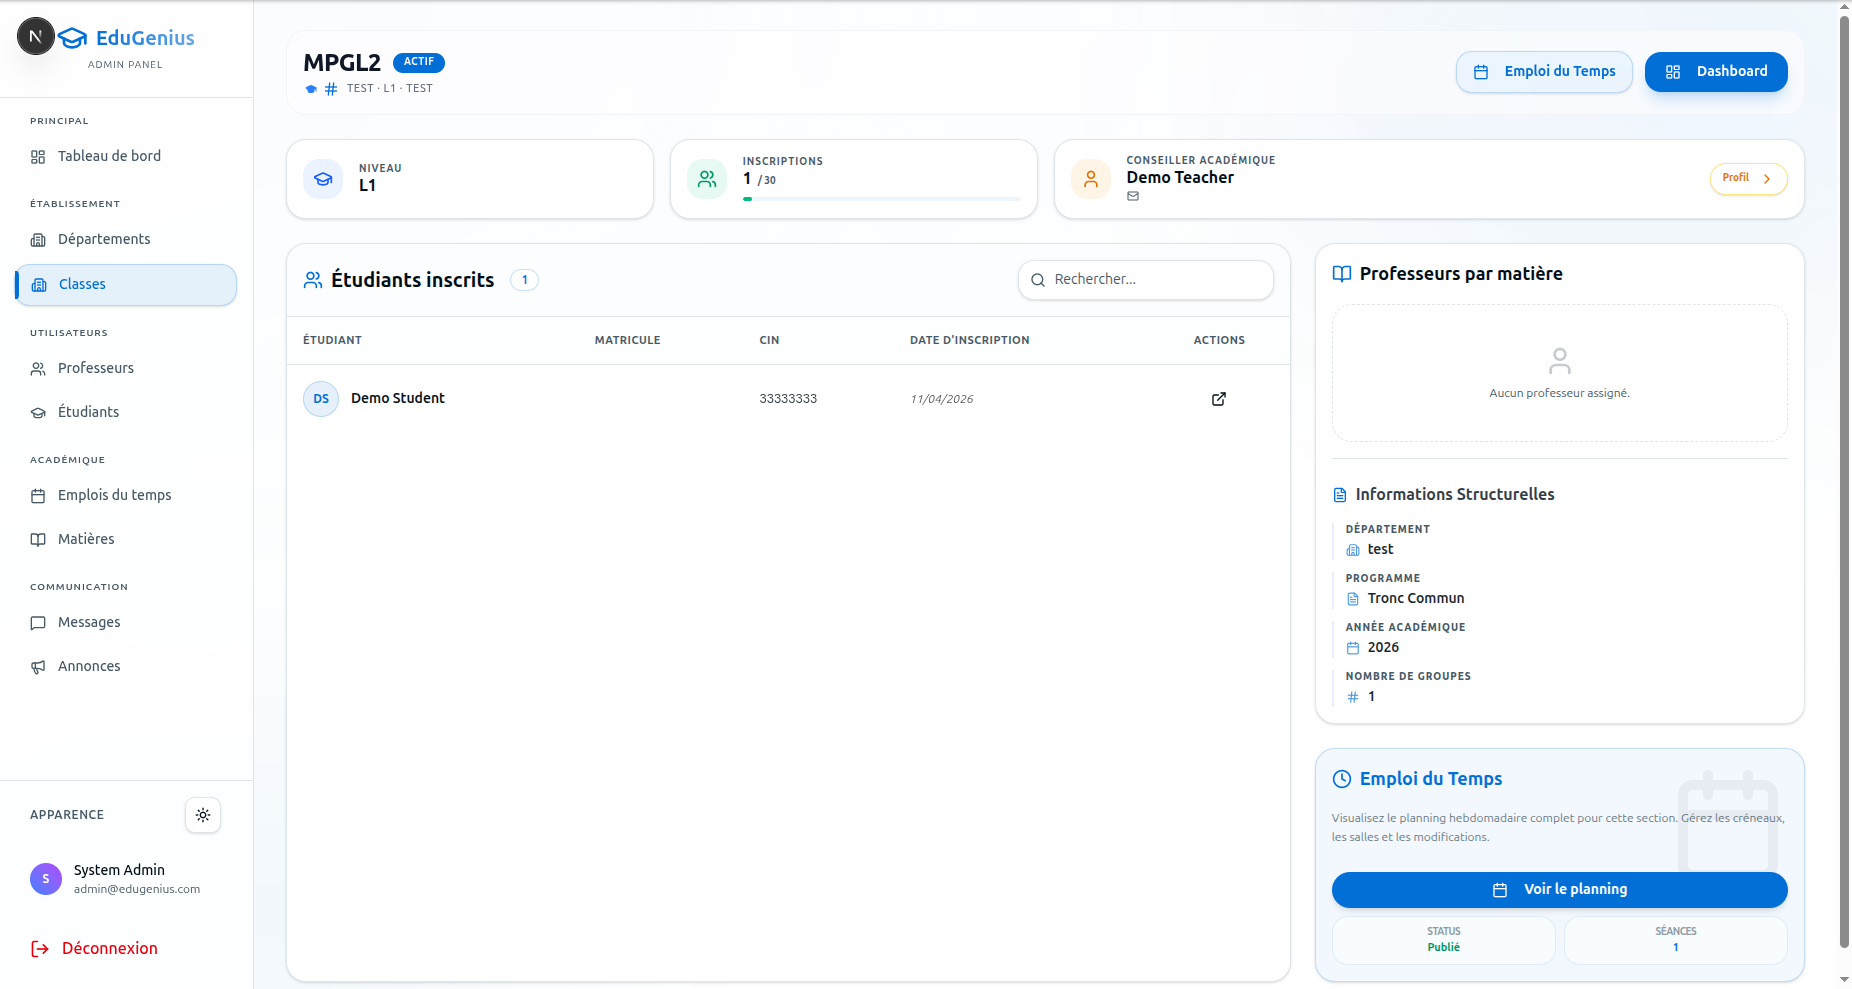
\includegraphics[width=\textwidth]{images/class_management_ui_2.png}
    \caption{Interface de création et d'édition des classes}
    \label{fig:class_form_ui}
\end{figure}

\subsection{Interface de planification des cours}

La création d'un emploi du temps suit un assistant en trois étapes : (1) informations générales (titre, année, semestre, classe/enseignant cible), (2) configuration des séances avec détection de conflits d'horaires et support de la récurrence, (3) récapitulatif avec validation et publication.

\begin{figure}[H]
    \centering
    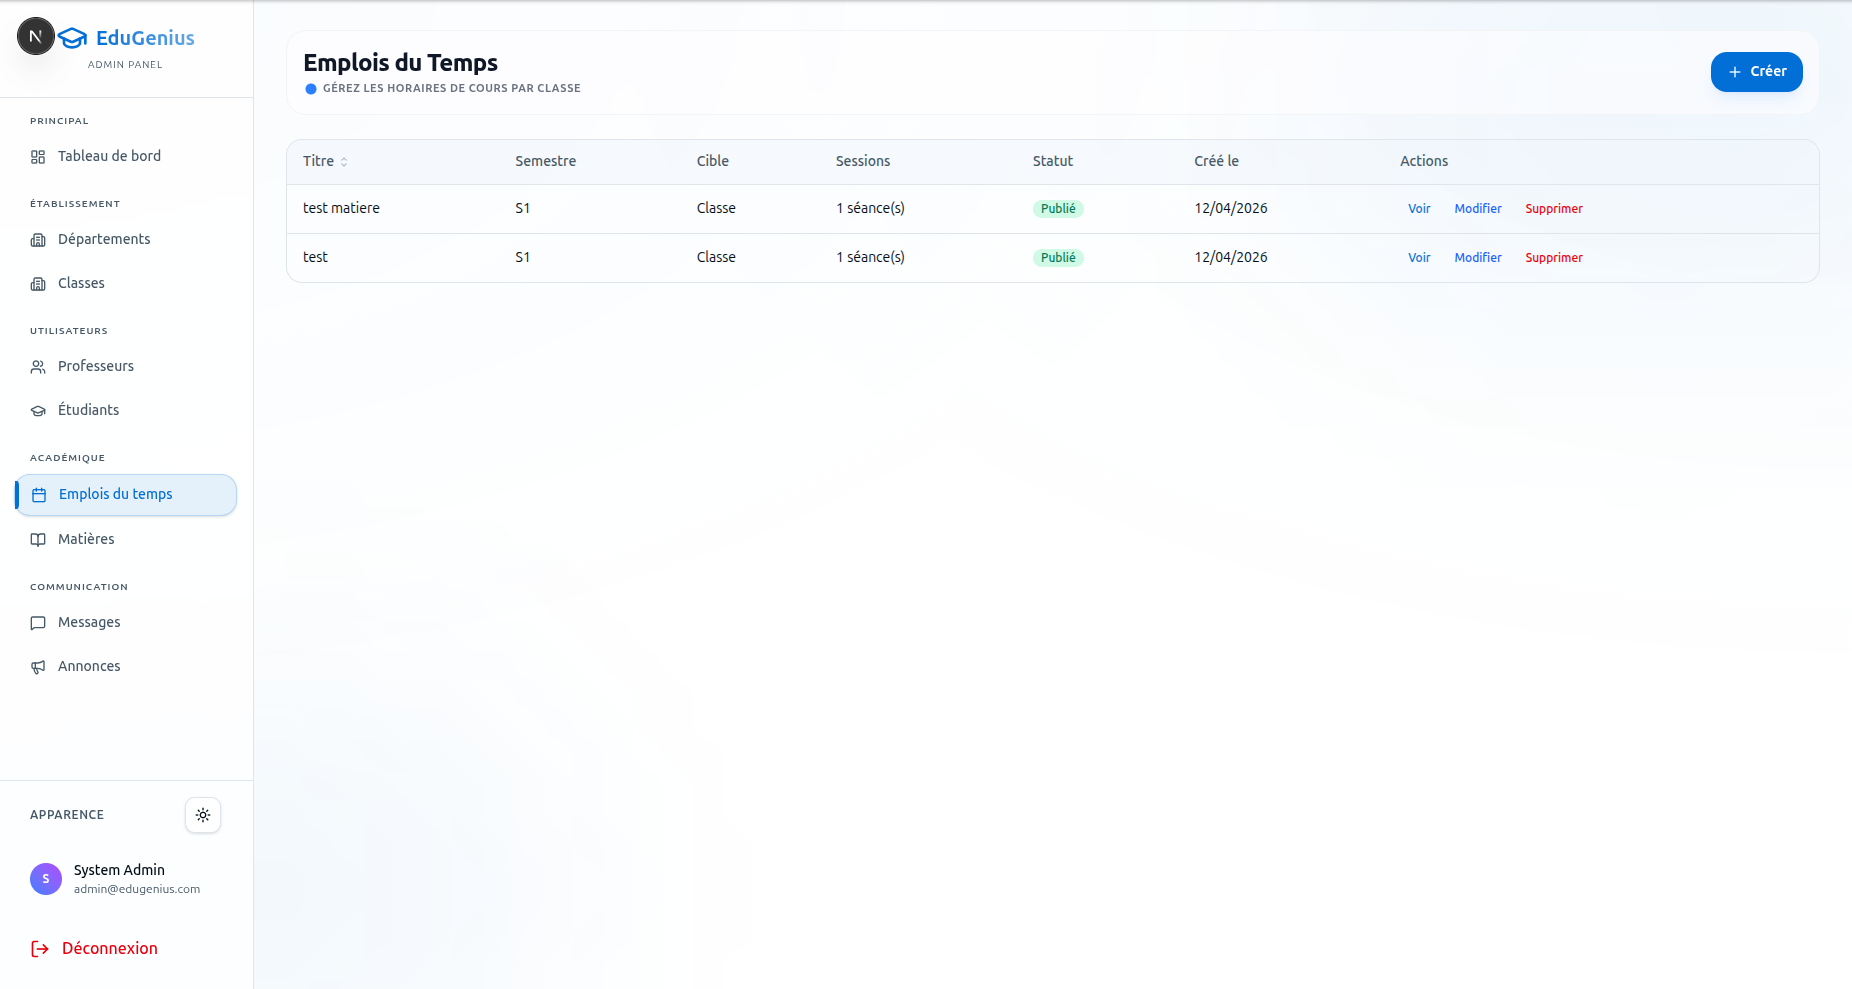
\includegraphics[width=\textwidth]{images/schedule_management_ui_1.png}
    \caption{Interface de planification : Informations générales}
    \label{fig:schedule_ui_1}
\end{figure}

\begin{figure}[H]
    \centering
    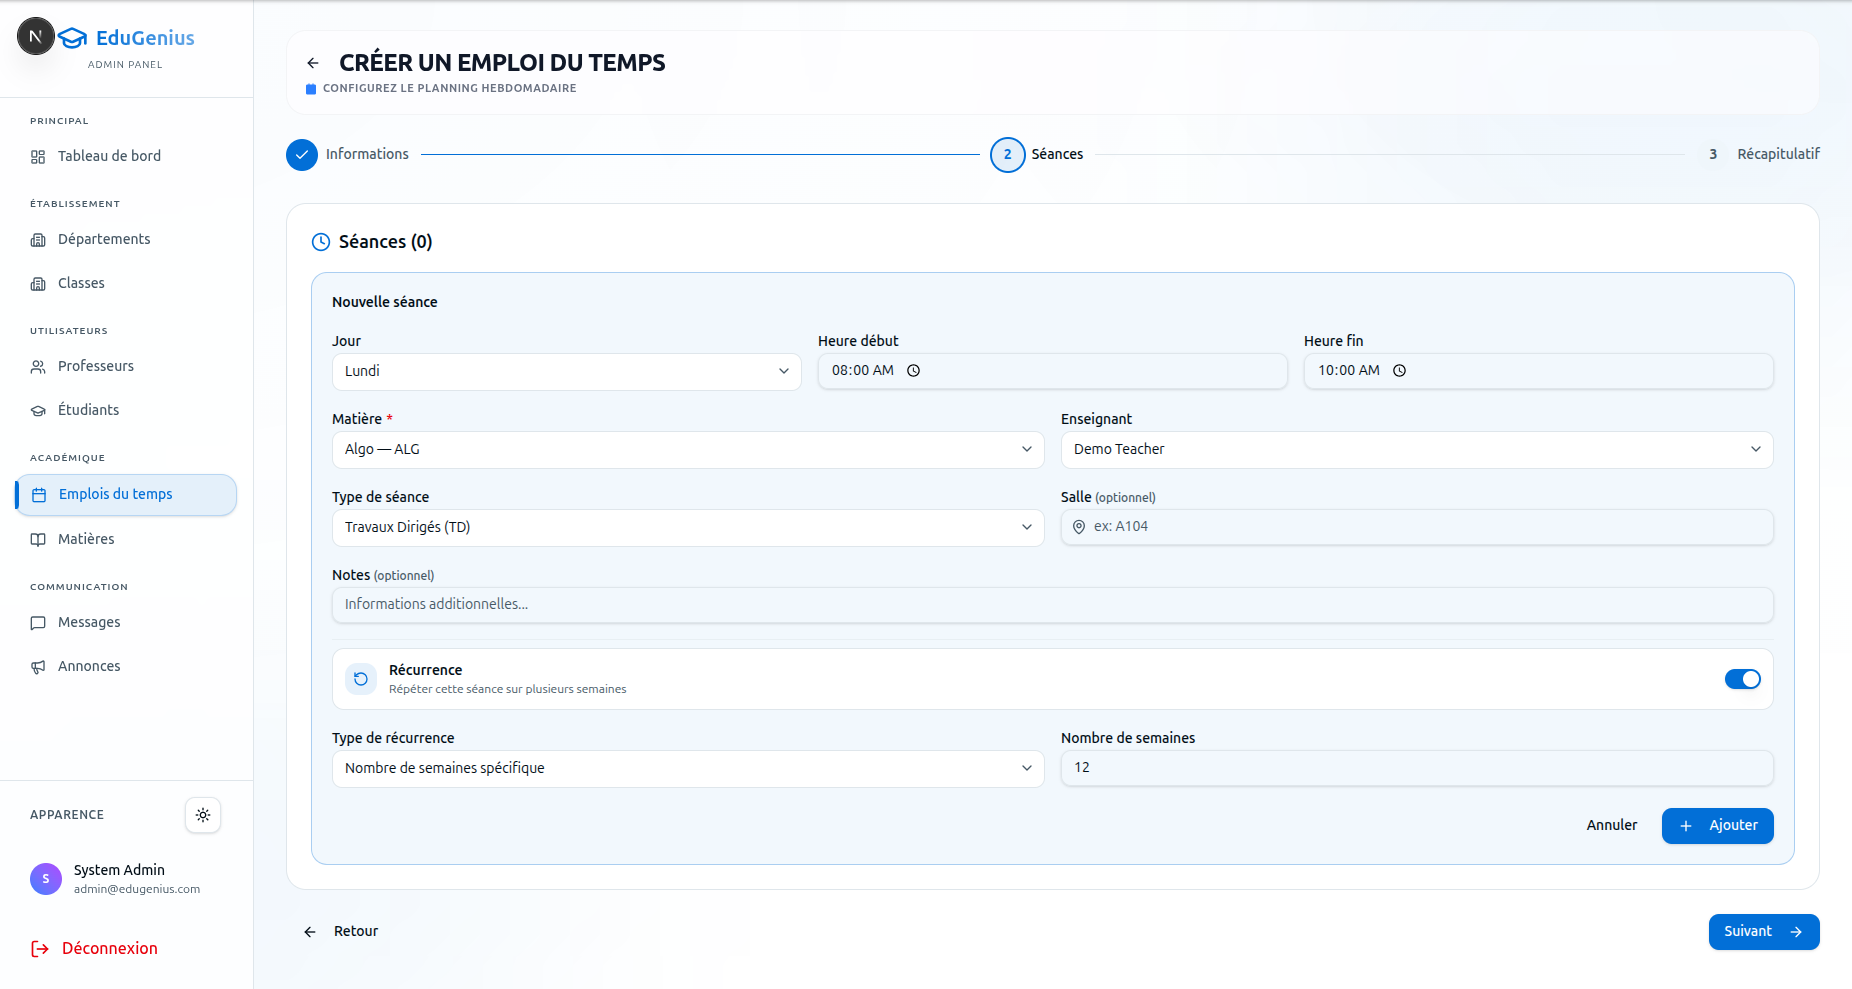
\includegraphics[width=\textwidth]{images/schedule_management_ui_2.png}
    \caption{Interface de planification : Configuration des séances}
    \label{fig:schedule_ui_2}
\end{figure}

\begin{figure}[H]
    \centering
    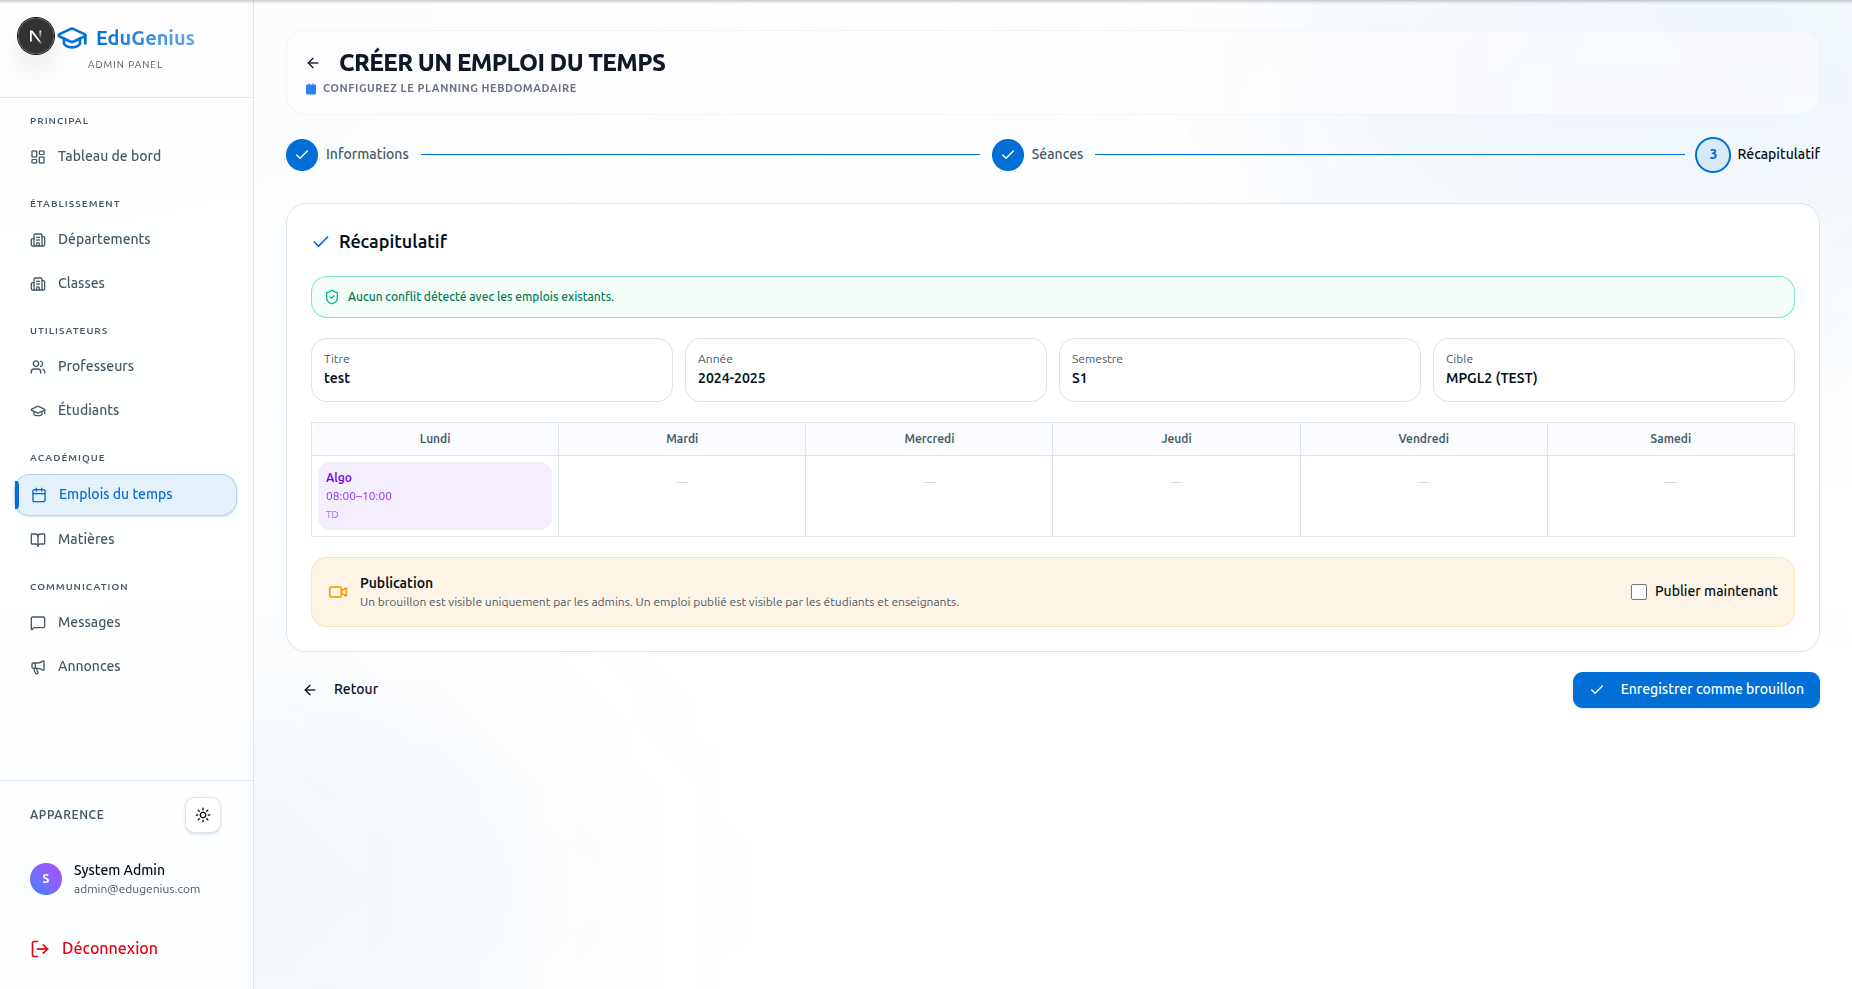
\includegraphics[width=\textwidth]{images/schedule_management_ui_3.png}
    \caption{Interface de planification : Récapitulatif et validation}
    \label{fig:schedule_ui_3}
\end{figure}

\subsection{Interface de supervision générale (Admin)}

Le tableau de bord de supervision offre un aperçu global de la plateforme : indicateurs clés (effectifs, classes, sessions en direct, taux de présence), sessions actives avec possibilité de rejoindre, dernières annonces et travaux soumis, distribution des effectifs par classe, et alertes système.

\begin{figure}[H]
    \centering
    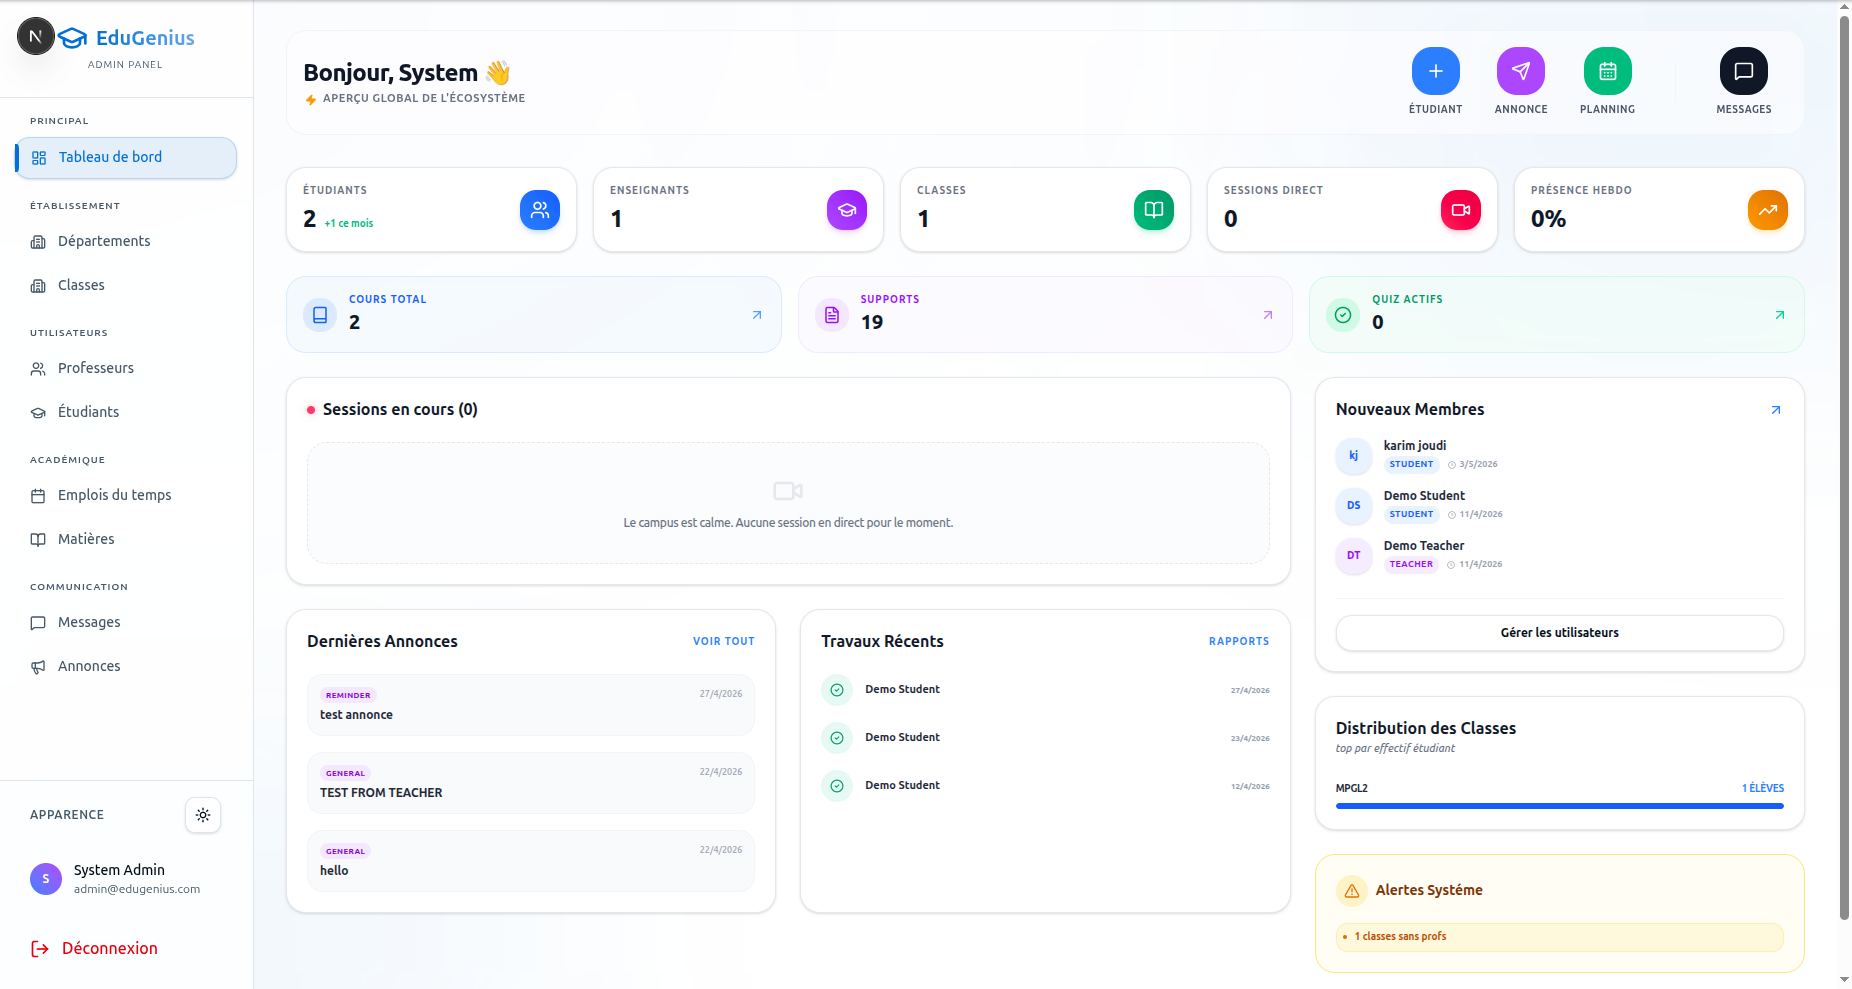
\includegraphics[width=\textwidth]{images/supervision_admin_ui.png}
    \caption{Tableau de bord de supervision}
    \label{fig:supervision_ui}
\end{figure}
\subsection{Interface de suivi de présence et historique}

L'historique de présence permet de filtrer par période et d'afficher les statistiques consolidées (taux de présence moyen, nombre de présents, retardataires et absents). Un tableau détaillé présente chaque session avec son taux d'assiduité, et un export CSV est disponible.

\begin{figure}[H]
    \centering
    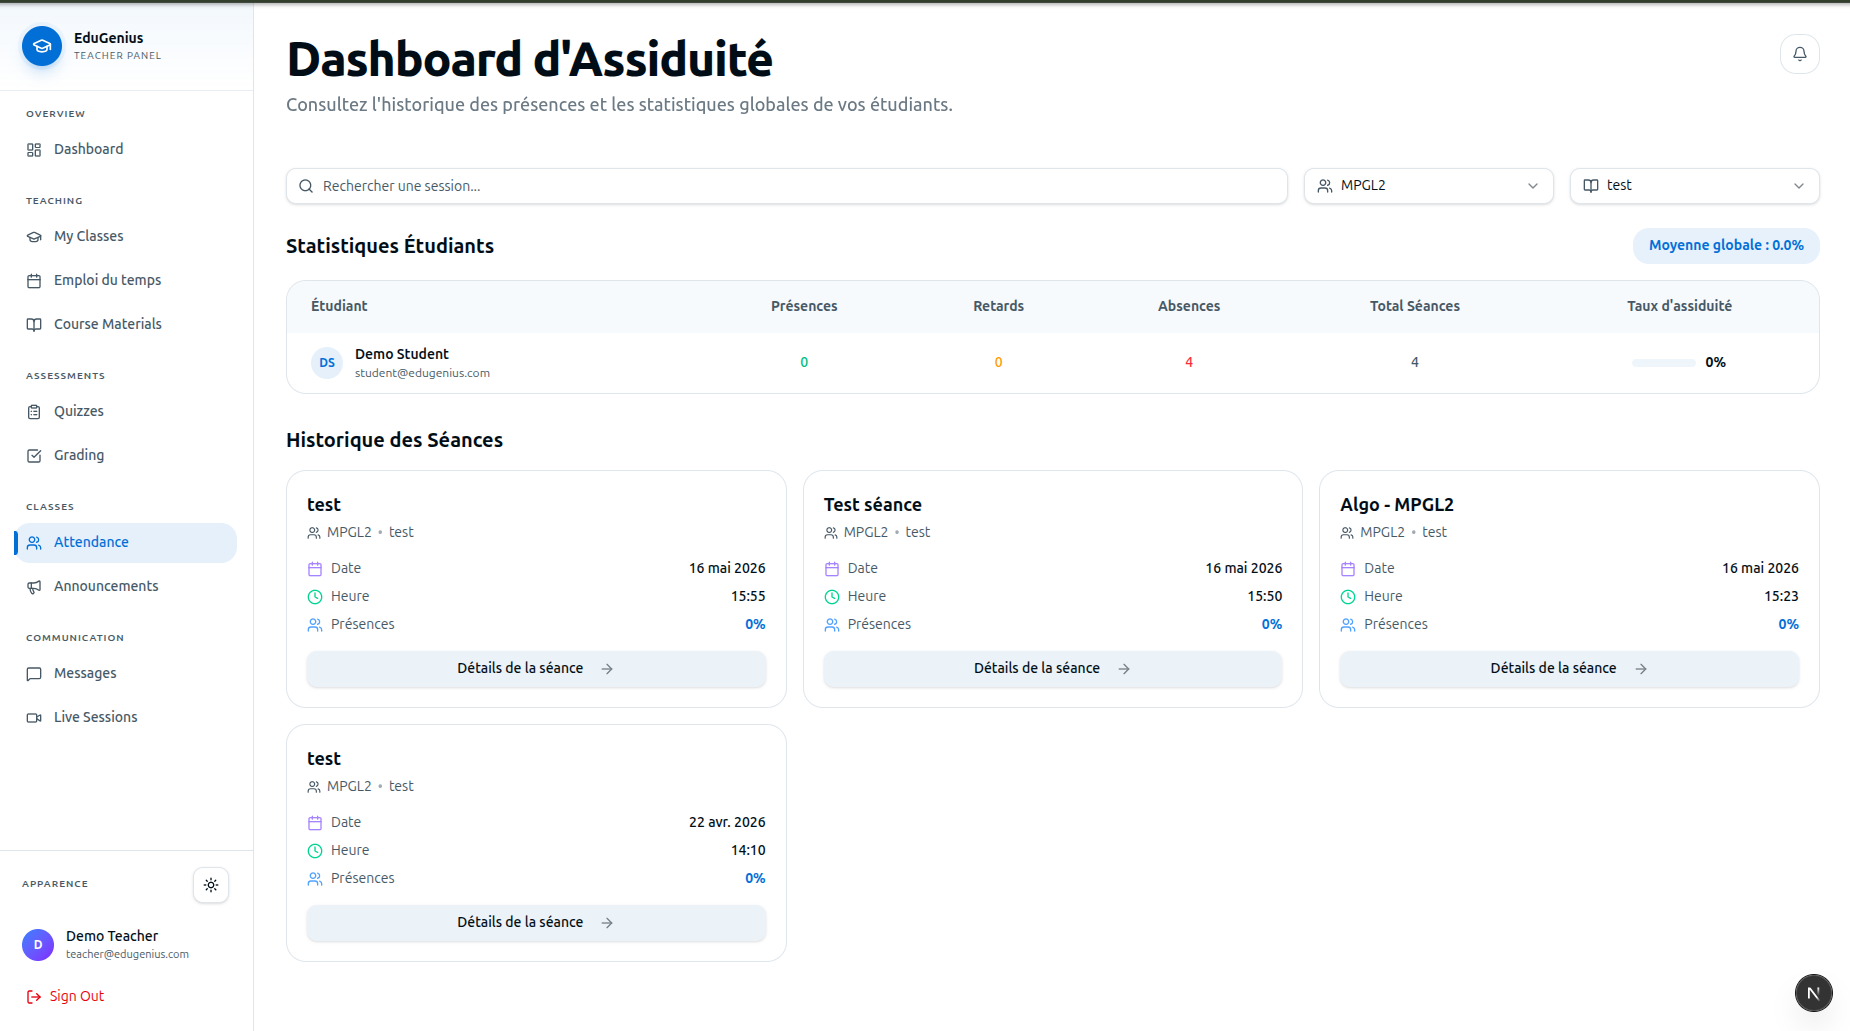
\includegraphics[width=\textwidth]{images/presence_ui.png}
    \caption{Historique des participations par étudiant/session}
    \label{fig:presence_ui}
\end{figure}

\subsection{Interface de replay (enregistrement)}

Les sessions enregistrées sont accessibles via un onglet dédié dans l'espace étudiant. Chaque enregistrement est présenté sous forme de carte avec le nom de la classe, le titre de la session, l'enseignant et la durée. L'interface propose également un onglet pour les sessions à venir avec indication du statut (planifié/en direct).

\begin{figure}[H]
    \centering
    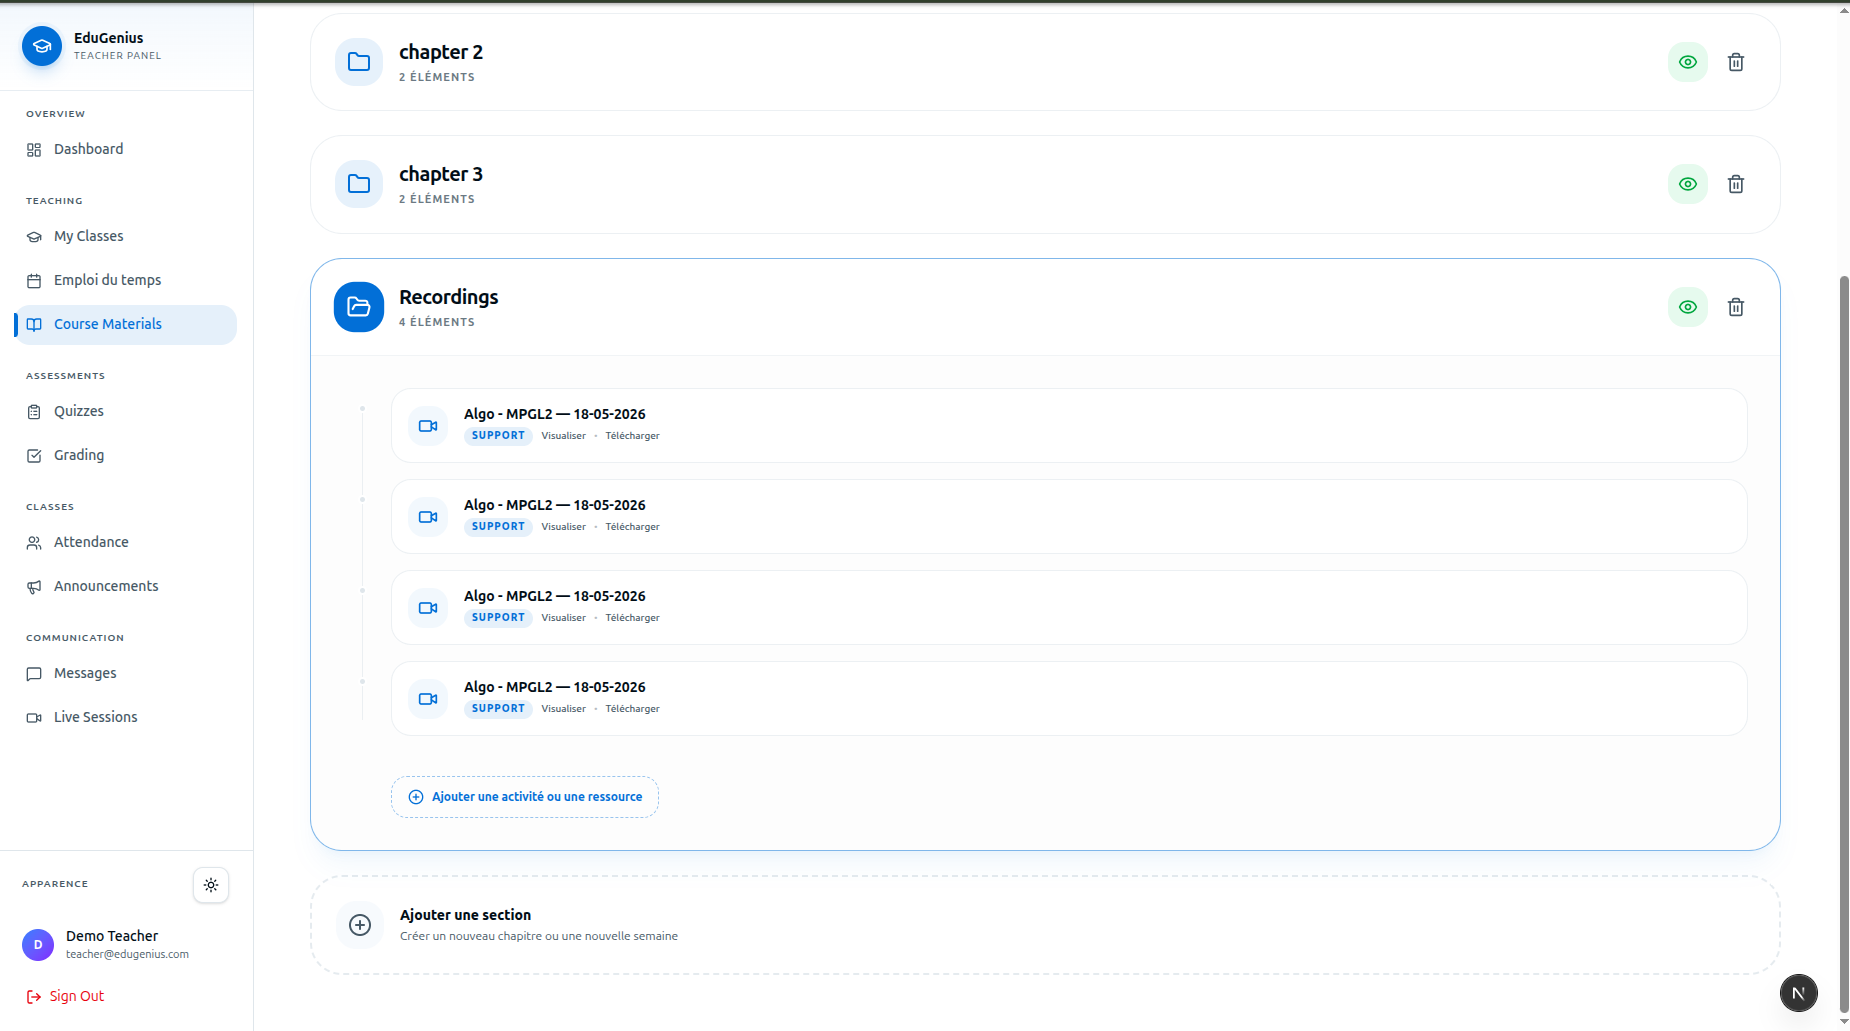
\includegraphics[width=\textwidth]{images/replay_ui_1.png}
    \caption{Interface de replay : Dossier des enregistrements disponibles par classe et matière}
    \label{fig:replay_list_ui}
\end{figure}

\section{Tests}
Cette phase de tests garantit la fiabilité des algorithmes de détection de présence et la robustesse de la gestion administrative des classes.

\subsection{Tests unitaires}
Nous avons mis en place des tests automatisés avec \textbf{Jest} pour valider la logique métier de calcul d'assiduité. La fonction \texttt{calculateAttendance} a été extraite et testée de manière isolée avec deux scénarios critiques :
\begin{itemize}
    \item \textbf{Validation des seuils} : Un étudiant participant à 30 minutes sur 60 (50\%) est marqué "Absent" car son taux est inférieur au seuil de 70\% (\texttt{attendanceThreshold}).
    \item \textbf{Détection des retards} : Un étudiant rejoignant la session à 09h20 pour un cours débutant à 09h00 est marqué "Late" car il dépasse la \texttt{gracePeriod} de 15 minutes.
\end{itemize}

\begin{figure}[H]
    \centering
    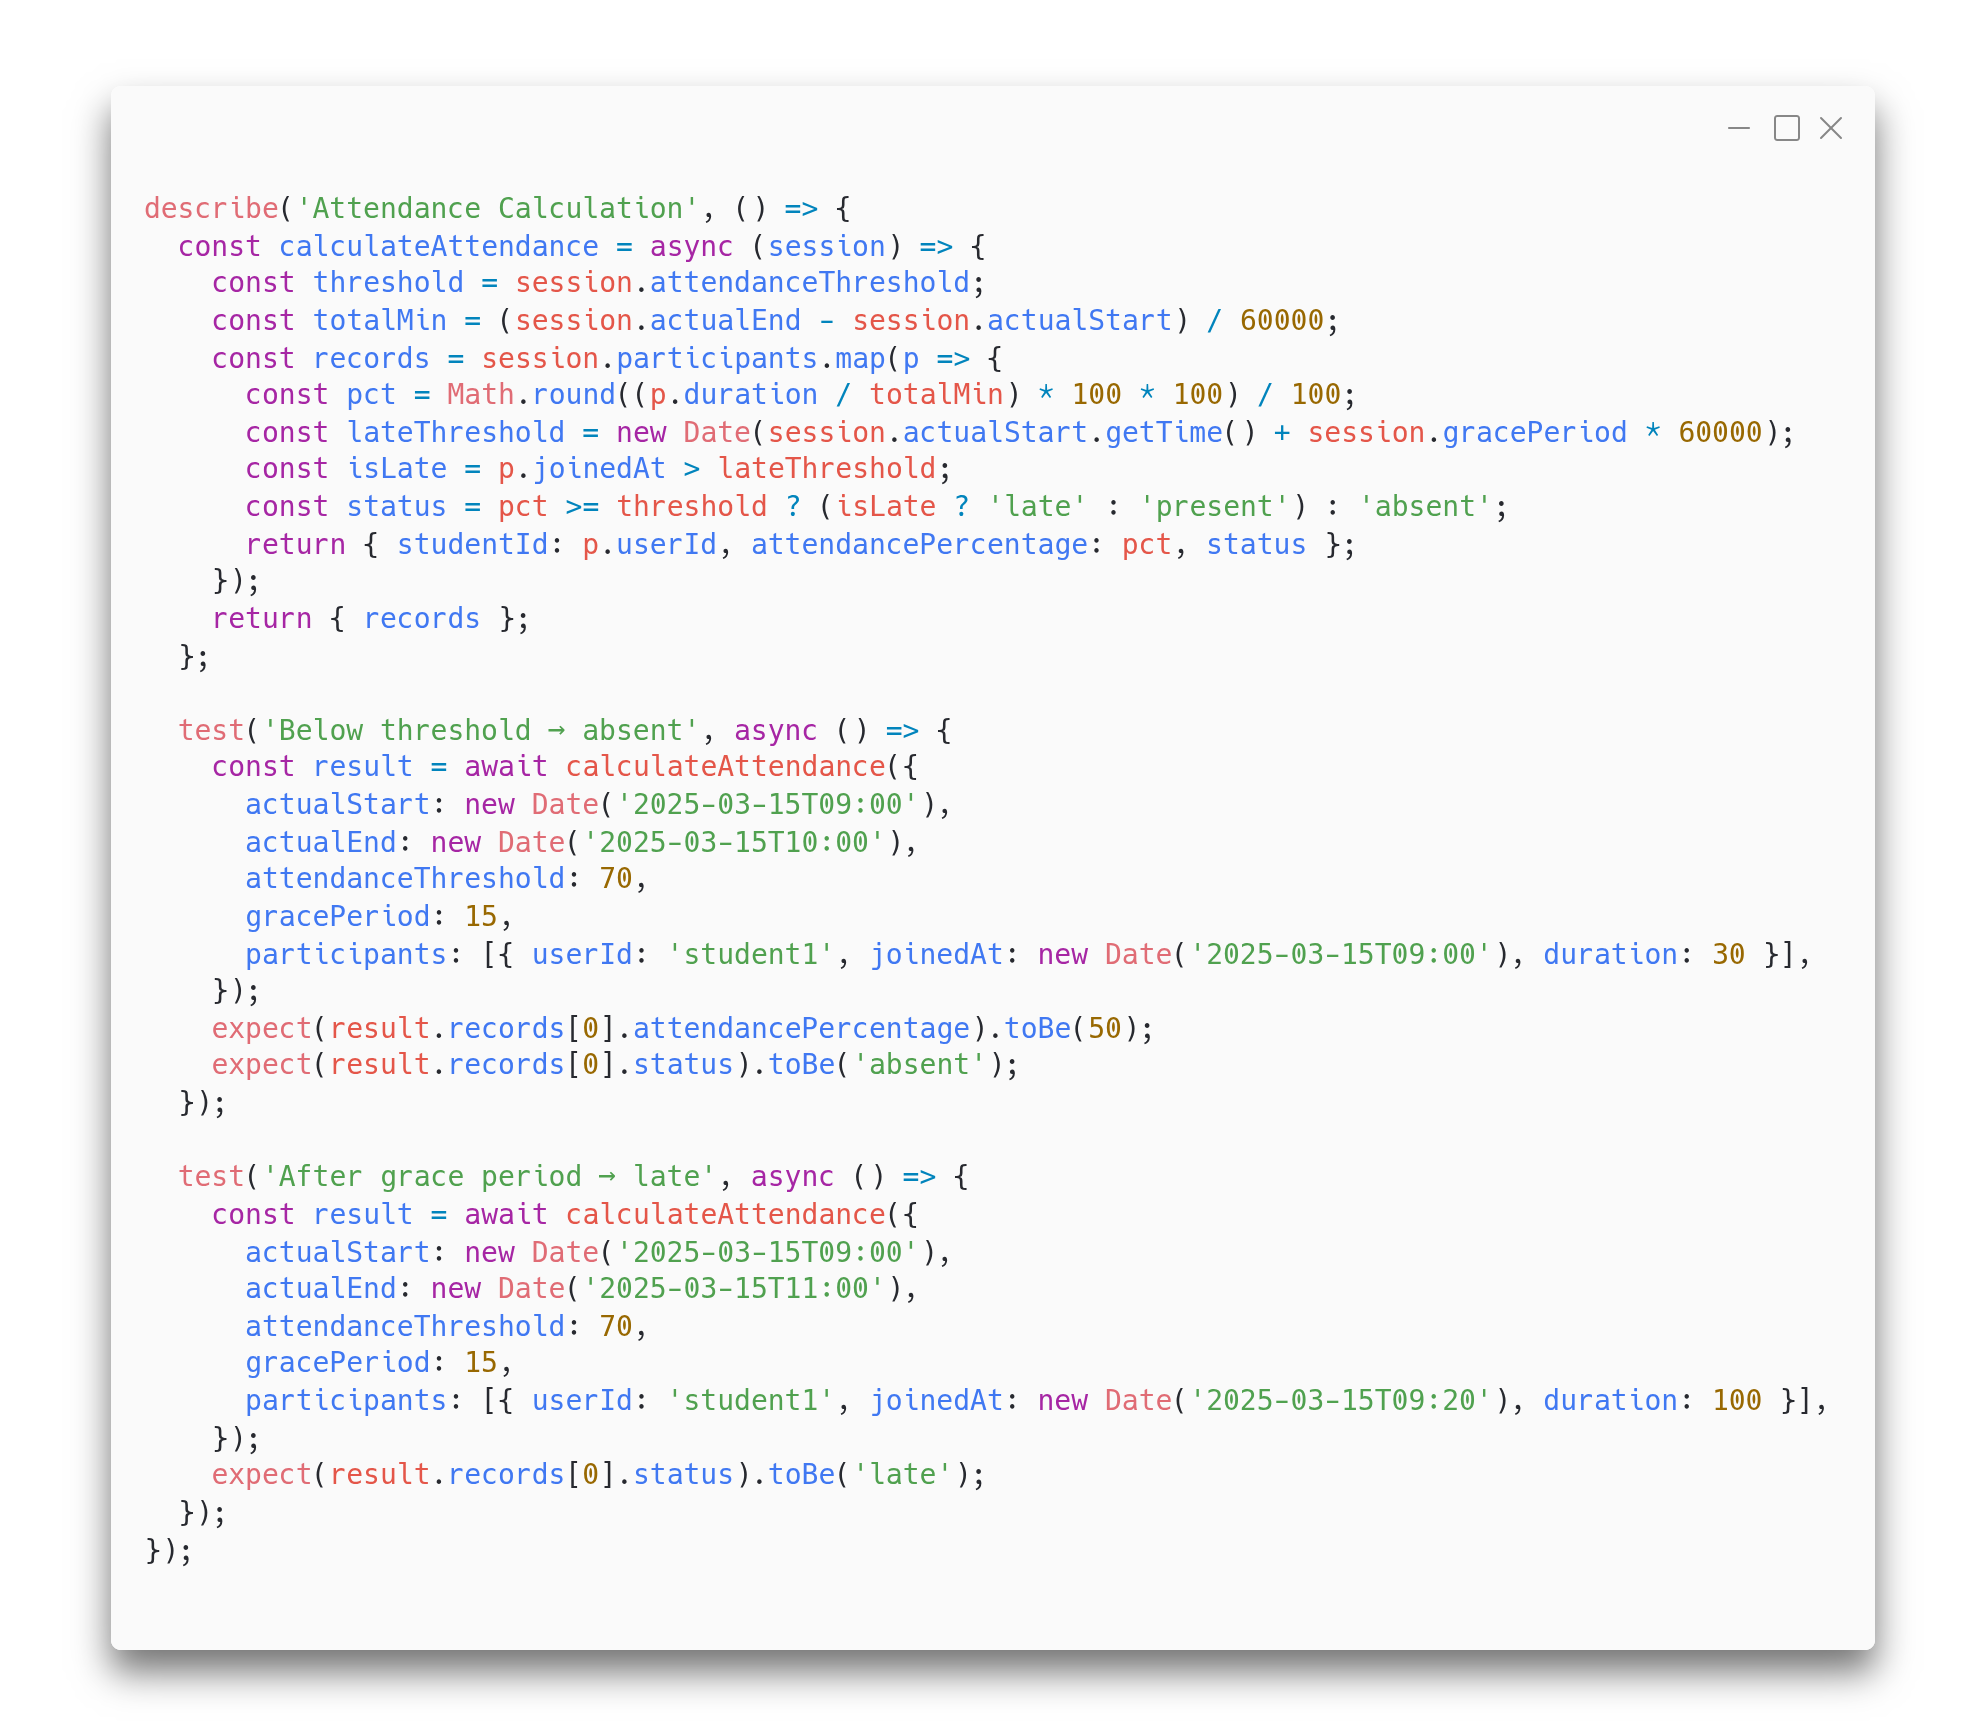
\includegraphics[width=0.9\textwidth]{images/attence_test.png}
    \caption{Extrait du code source du test unitaire (Jest)}
    \label{fig:unit_test_code_s2}
\end{figure}

\subsection{Tests d’intégration}
Les tests d'intégration valident la communication entre le client HTTP, le serveur Express et la base de données MongoDB. Le test principal a porté sur la création d'un emploi du temps via l'endpoint \texttt{POST /api/admin/schedules}.

À l'aide de l'outil \textbf{Postman}, nous avons soumis une requête authentifiée avec le token JWT d'un administrateur, contenant les informations de l'emploi du temps (titre, année universitaire, semestre, classe cible, séances). Le système a validé avec succès la chaîne complète : extraction du token $\rightarrow$ vérification des droits d'administrateur $\rightarrow$ validation et persistance dans MongoDB $\rightarrow$ génération automatique des URLs de visioconférence $\rightarrow$ retour de l'objet créé.

Comme illustré dans la figure \ref{fig:integration_test_s2}, le serveur retourne un statut \texttt{201 Created} accompagné de l'objet JSON de l'emploi du temps. La réponse inclut l'identifiant unique généré par MongoDB (\texttt{\_id}), les séances planifiées avec leurs créneaux horaires, ainsi que l'URL de visioconférence Jitsi automatiquement générée (\texttt{meetingUrl}). Ce test confirme le bon fonctionnement du module de planification, brique centrale de l'organisation pédagogique du sprint.

\begin{figure}[H]
    \centering
    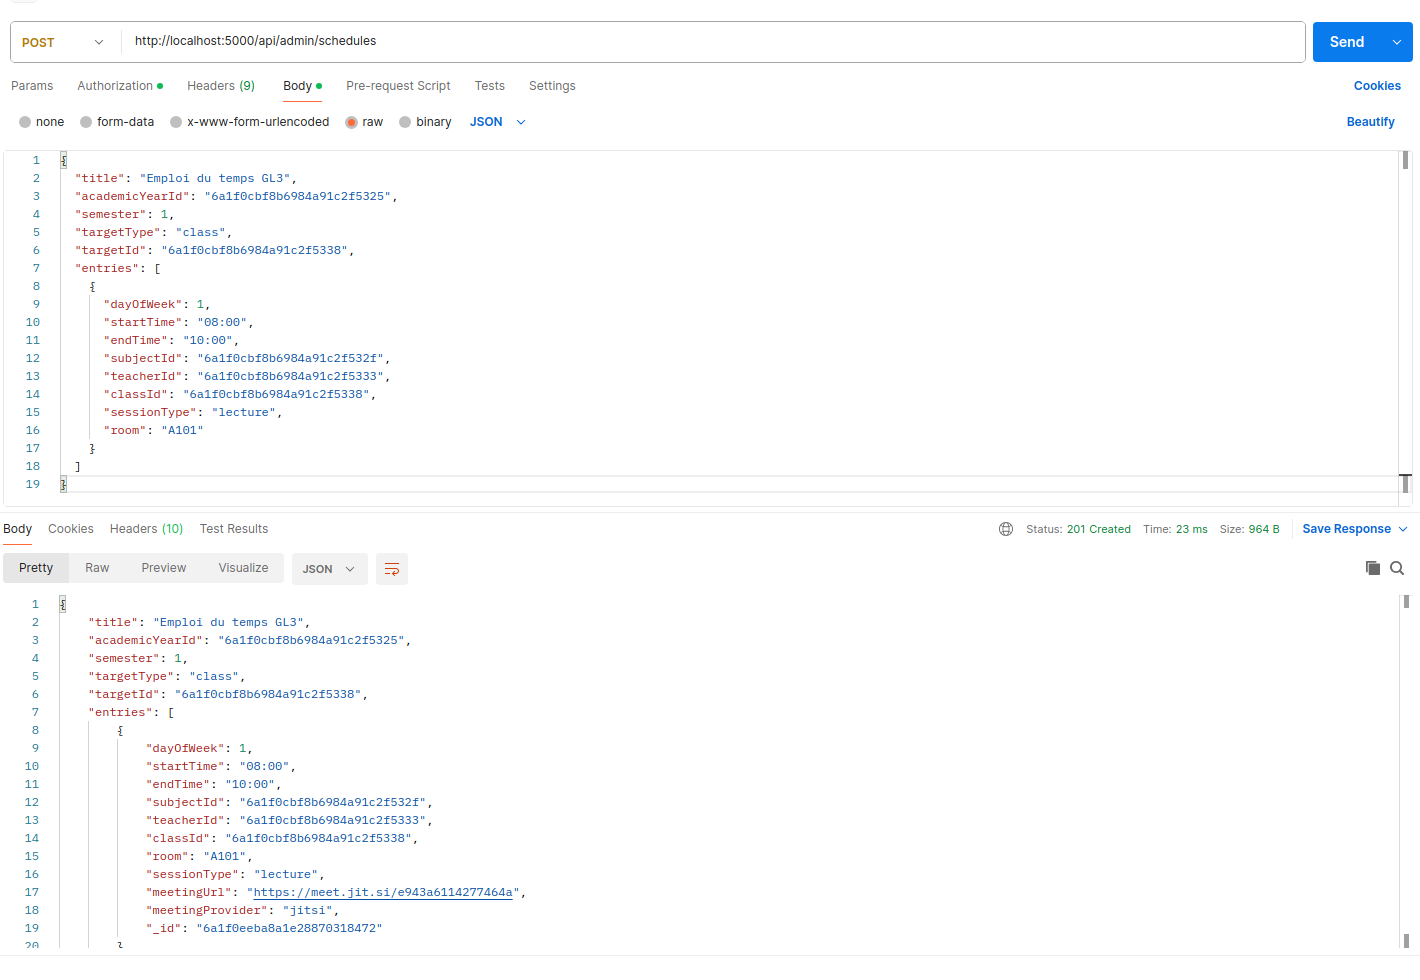
\includegraphics[width=0.8\textwidth]{images/integration_test_sprint_2.png}
    \caption{Validation du point d'entrée POST /api/admin/schedules via Postman}
    \label{fig:integration_test_s2}
\end{figure}

\subsection{Tests fonctionnels}
Les tests de bout en bout ont validé le parcours utilisateur complet de création et configuration d'une classe :
\begin{enumerate}
    \item L'administrateur accède à la page \texttt{/admin/classes} et clique sur \textbf{Nouvelle Classe}.
    \item Il remplit le formulaire (nom, code, département, niveau, capacité) et soumet.
    \item La classe apparaît dans la grille avec son code et son niveau.
    \item L'administrateur inscrit des étudiants via la modale d'inscription avec recherche.
\end{enumerate}

\begin{figure}[H]
    \centering
    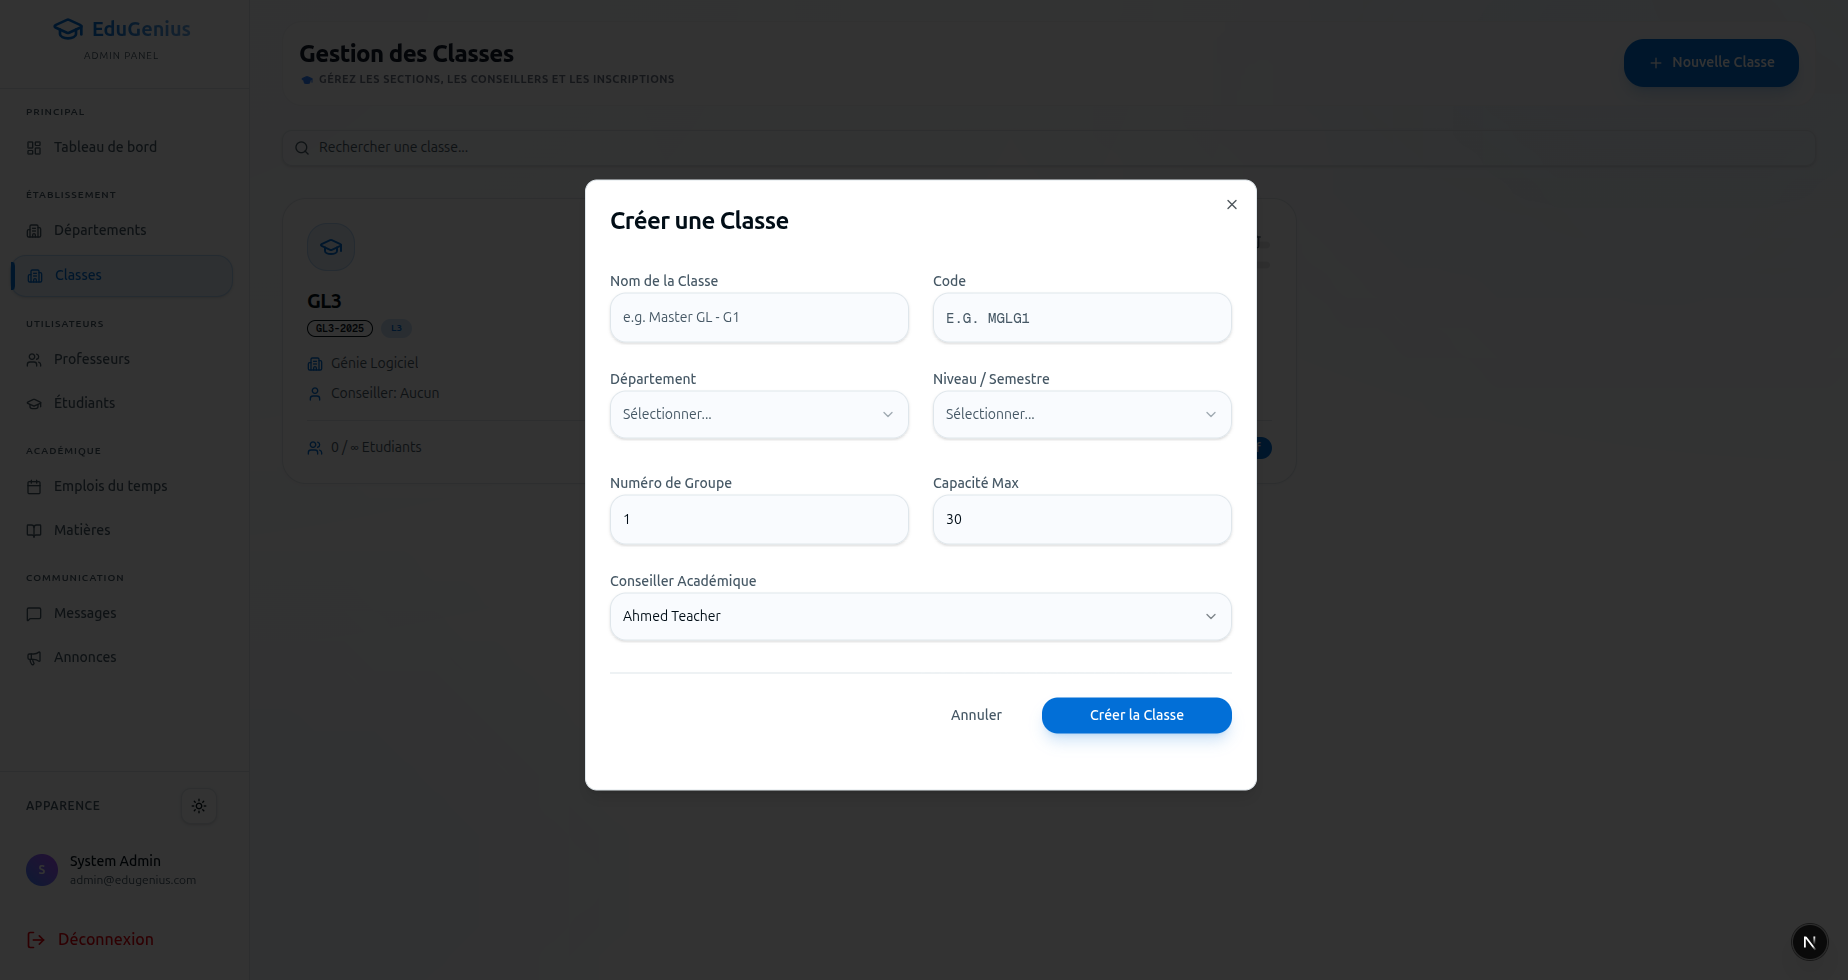
\includegraphics[width=0.9\textwidth]{images/functional_test_sprint_2.png}
    \caption{Parcours fonctionnel de création et configuration d'une classe}
    \label{fig:functional_test_s2}
\end{figure}

\section{Conclusion}

Ce deuxième sprint a permis de doter EduGenius d’un socle complet de gestion des classes, de planification et de visioconférence. L’ensemble des onze user stories (US-06 à US-16) a été développé et testé avec succès, offrant une base solide pour les fonctionnalités pédagogiques du sprint 3.

% \chapter{Sprint 3 : Gestion des Microservices}

\section{Introduction}
Le Sprint 3 est dédié à l'implémentation des services transverses qui apportent de l'intelligence et des capacités de stockage à la plateforme. Bien que l'architecture soit monolithique, ces services sont conçus de manière modulaire, simulant une architecture de microservices.

\section{Backlog du Sprint 3}
\begin{itemize}
    \item \textbf{US-07} : Intégration du service de stockage AWS S3.
    \item \textbf{US-08} : Mise en place du service d'IA (Gemini/Ollama).
    \item \textbf{US-09} : Développement du service de communication temps réel (Socket.io).
\end{itemize}

\section{Analyse}
\subsection{Diagramme de cas d'utilisation}
L'Enseignant upload des fichiers PDF qui sont stockés sur le cloud. Le système traite ces fichiers pour générer des services à valeur ajoutée (Résumés).

\subsection{Description textuelle des cas d'utilisation}
L'utilisateur envoie un fichier. Le service S3 gère l'upload et renvoie une URL. Le service IA récupère le contenu pour analyse. Le service Socket notifie les utilisateurs des nouveaux contenus disponibles.

\section{Conception}
\subsection{Diagrammes de séquence}
Le diagramme de séquence montre l'orchestration entre le \texttt{CourseController}, le \texttt{S3Service} et le \texttt{AiService}.
\begin{figure}[H]
    \centering
    \fbox{Placeholder: Diagramme de Séquence - Flux de Services}
    \caption{Interactions entre les services backend}
\end{figure}

\subsection{Diagramme de classes}
Les classes \texttt{S3Utils}, \texttt{AiService} et \texttt{SocketHandler} encapsulent la logique de communication avec les APIs tierces.

\subsection{Représentation graphique de la base de données}
Mise à jour des schémas \texttt{Course} et \texttt{StudyMaterial} pour inclure les URLs S3 et les résultats des traitements IA.

\section{Réalisation}
\subsection{Interface d'Upload vers AWS S3}
Une barre de progression indique l'état de l'upload vers le cloud Amazon.
\begin{figure}[H]
    \centering
    \fbox{Placeholder: Capture d'écran - File Upload}
    \caption{Interface de dépôt de documents}
\end{figure}

\subsection{Module de Communication Temps Réel}
Implémentation de Socket.io pour la messagerie instantanée au sein des classes.

\section{Tests}
\subsection{Tests unitaires}
Validation des fonctions d'extraction de texte PDF.
\subsection{Tests d'intégration}
Vérification de la connectivité avec les buckets AWS S3 et l'API Gemini.
\subsection{Tests fonctionnels}
Test de réception des notifications en temps réel sur plusieurs clients simultanés.

\section{Conclusion}
Les services de base étant opérationnels, le sprint suivant se focalisera sur l'exposition de ces services via des endpoints REST et la modélisation fine des données.

% \chapter{Sprint 4 : Gestion des Endpoints et des Modèles}

\section{Introduction}
Ce sprint se focalise sur le développement de l'API RESTful et la définition précise des modèles de données Mongoose pour assurer une persistence cohérente et performante.

\section{Backlog du Sprint 4}
\begin{itemize}
    \item \textbf{US-10} : Développement des contrôleurs pour les Cours et les Quiz.
    \item \textbf{US-11} : Définition des schémas de données complexes (Attendance, Submissions).
    \item \textbf{US-12} : Mise en place des routes API sécurisées.
\end{itemize}

\section{Analyse}
\subsection{Diagramme de cas d'utilisation}
L'Enseignant crée des examens et des quiz. L'Étudiant soumet ses travaux. L'Administrateur génère des PV de notes.

\subsection{Description textuelle des cas d'utilisation}
L'enseignant définit les paramètres d'un quiz (temps, questions). L'étudiant répond aux questions. Le système enregistre les réponses dans la collection \texttt{StudentQuizAttempt} et calcule le score automatiquement.

\section{Conception}
\subsection{Diagrammes de séquence}
Le diagramme de séquence pour la soumission d'un examen illustre le flux depuis le client jusqu'à la validation et l'enregistrement des notes en base de données.

\subsection{Diagramme de classes}
Détail des modèles \texttt{Quiz}, \texttt{Question}, \texttt{Exam}, \texttt{Submission} et \texttt{Grade}.

\subsection{Représentation graphique de la base de données}
Schéma complet de la base de données MongoDB illustrant les relations entre les collections académiques et les collections d'évaluation.
\begin{figure}[H]
    \centering
    \fbox{Placeholder: Schéma ER / MongoDB}
    \caption{Architecture des données d'eduGenius}
\end{figure}

\section{Réalisation}
\subsection{Interface de Création de Quiz}
Formulaire dynamique permettant d'ajouter des questions, des options et de définir la bonne réponse.
\begin{figure}[H]
    \centering
    \fbox{Placeholder: Capture d'écran - Quiz Creator}
    \caption{Interface de création d'évaluations}
\end{figure}

\subsection{Implémentation des Contrôleurs REST}
Développement de la logique métier dans \texttt{QuizController.js} et \texttt{ExamController.js}.

\section{Tests}
\subsection{Tests unitaires}
Validation de la logique de calcul des scores des quiz.
\subsection{Tests d'intégration}
Test des endpoints de soumission de travaux avec gestion des fichiers joints.
\subsection{Tests fonctionnels}
Vérification de la génération correcte des moyennes dans le module PV.

\section{Conclusion}
L'API étant complète et robuste, le dernier sprint sera consacré à l'interface utilisateur finale et à l'intégration poussée de l'IA.

% \chapter{Sprint 5 : Tableau de bord et IA}

\section{Introduction}
L'ultime sprint du projet se concentre sur l'expérience utilisateur finale, avec la réalisation des tableaux de bord interactifs et l'intégration profonde des fonctionnalités d'IA générative.

\section{Backlog du Sprint 5}
\begin{itemize}
    \item \textbf{US-13} : Développement des Dashboards (Admin, Teacher, Student).
    \item \textbf{US-14} : Intégration de la visioconférence (Daily.co).
    \item \textbf{US-15} : Finalisation des générateurs de résumés et de quiz IA.
\end{itemize}

\section{Analyse}
\subsection{Diagramme de cas d'utilisation}
L'Étudiant consulte son dashboard pour voir sa progression (XP). L'Enseignant lance une session vidéo. L'Administrateur surveille les statistiques globales.

\subsection{Description textuelle des cas d'utilisation}
L'enseignant clique sur "Générer Résumé". Le système appelle l'API Gemini, traite le résultat et l'affiche à l'écran. L'étudiant peut alors consulter ce résumé à côté de son support de cours.

\section{Conception}
\subsection{Diagrammes de séquence}
Le diagramme de séquence pour le lancement d'un Live montre l'interaction avec l'API Daily.co pour obtenir un token de salle.

\subsection{Diagramme de classes}
Classes \texttt{AIQuizController}, \texttt{AISummaryController} et les composants React du Dashboard.

\subsection{Représentation graphique de la base de données}
Documents stockant les résumés générés (\texttt{AISummary}) et les flashcards.

\section{Réalisation}
\subsection{Dashboard Étudiant avec Gamification}
Interface affichant les points d'expérience (XP), le GPA et les cours récents.
\begin{figure}[H]
    \centering
    \fbox{Placeholder: Capture d'écran - Student Dashboard}
    \caption{Tableau de bord intelligent de l'étudiant}
\end{figure}

\subsection{Interface de Visioconférence Intégrée}
Salle de classe virtuelle avec chat et liste des participants en temps réel.
\begin{figure}[H]
    \centering
    \fbox{Placeholder: Capture d'écran - Live Session}
    \caption{Module de visioconférence Daily.co}
\end{figure}

\section{Tests}
\subsection{Tests unitaires}
Tests des fonctions de formatage des réponses de l'IA.
\subsection{Tests d'intégration}
Validation de la persistance des résumés générés dans MongoDB.
\subsection{Tests fonctionnels}
Scénario complet : Upload d'un PDF $\rightarrow$ Génération d'un résumé $\rightarrow$ Consultation par l'étudiant $\rightarrow$ Passage du quiz lié.

\section{Conclusion}
Le Sprint 5 clôture la phase de développement avec une plateforme complète, intelligente et fonctionnelle, prête pour la mise en production.

% \chapter*{Conclusion Générale}
\phantomsection
\addcontentsline{toc}{chapter}{Conclusion Générale}

Le projet \textbf{eduGenius} a permis de concevoir et de réaliser une plateforme éducative innovante intégrant les dernières avancées en intelligence artificielle générative. Au cours de ce travail, nous avons pu relever les défis liés à la gestion du temps réel, au stockage cloud et à l'interaction avec des modèles de langage complexes dans un environnement agile.

Les objectifs fixés au début du projet ont été atteints, notamment la création d'un écosystème fluide pour les enseignants et les étudiants. La méthodologie Scrum a prouvé son efficacité pour piloter un projet aux technologies changeantes, permettant de transformer chaque besoin en un incrément fonctionnel et testé.

Cependant, ce projet reste ouvert à des améliorations futures. Nous envisageons d'intégrer un tutorat personnalisé par l'IA capable de répondre aux questions des étudiants en temps réel pendant les sessions live, ainsi que d'approfondir l'analyse prédictive pour identifier précocement les étudiants en difficulté.

Ce stage a été une expérience enrichissante, me permettant de consolider mes compétences en développement Full-stack (MERN) et d'explorer le potentiel de l'IA dans le secteur de l'éducation.


% --- References ---
\newpage
\phantomsection
\addcontentsline{toc}{chapter}{Bibliographie}
\nocite{*}
\bibliographystyle{plain}
\bibliography{biblio}

\chapter*{Webographie}
\addcontentsline{toc}{chapter}{Webographie}
\begin{itemize}
    \item \url{https://nextjs.org/docs}
    \item \url{https://expressjs.com/}
    \item \url{https://www.mongodb.com/docs/}
    \item \url{https://aws.amazon.com/s3/}
    \item \url{https://daily.co/}
    \item \url{https://ollama.com/}
\end{itemize}

\end{document}
